\documentclass[a4paper]{report}
\usepackage{natbib}
\bibpunct{[}{]}{,}{a}{}{;}
\usepackage{fancyheadings}
\usepackage{iamdip}
\usepackage[pdftex]{graphicx}
\usepackage{amsmath}
\usepackage{amsthm}
\usepackage{amssymb}
\usepackage{amsfonts}
\usepackage{url}
\usepackage{hyperref}
\usepackage{listings}
\usepackage{pdfpages}
\usepackage{lingmacros}
\usepackage{tree-dvips}
\usepackage{mathpazo}
\usepackage[english]{babel}
\usepackage{fontspec}
\usepackage{algpseudocode}
\usepackage{algorithm}
\usepackage{mathrsfs}
\usepackage{dsfont}
\usepackage{graphicx}
\usepackage{wasysym}
\usepackage[hypcap]{caption}
\usepackage{subfigure}
\usepackage{float}
\usepackage{mathtools}
\usepackage{mdwlist}
\usepackage{gensymb}
\usepackage{array}
\usepackage{multirow}
\usepackage[hmargin=3cm]{geometry}
\usepackage{boxedminipage}

\renewcommand{\algorithmicforall}{\textbf{Foreach}}
\newcommand{\init}{\textbf{INIT }}
\newcommand{\pluseq}{\mathrel{+}=}
\newcommand{\asteq}{\mathrel{*}=}
\newcommand{\myto}{\textbf{TO }}
\newcommand*\colvec[3][]{
    \begin{pmatrix}\ifx\relax#1\relax\else#1\\\fi#2\\#3\end{pmatrix}
}
\newcommand{\myparagraph}[1]{\paragraph{#1}\mbox{}\\}
\DeclarePairedDelimiter\ceil{\lceil}{\rceil}
\DeclarePairedDelimiter\floor{\lfloor}{\rfloor}

\headrulewidth 0.5pt \addtolength{\headheight}{5pt}

\lhead[\fancyplain{}{\rm\thepage}]{\fancyplain{}{\rightmark}}
\rhead[\fancyplain{}{\leftmark}]{\fancyplain{}{\rm\thepage}}
\cfoot{}

\graphicspath{{../Figures/}}

\begin{document}

\pagestyle{fancyplain} \thispagestyle{empty}

\title{An Interactive Shader for Natural Diffraction Gratings}
\author{Michael Single}
\betreuer{Prof. Dr. Matthias Zwicker}
\ort{Bern}
\datum{2014}

\pagenumbering{roman} \setcounter{page}{1}
\maketitle

\newpage
\thispagestyle{empty}
\vspace{8cm}
\noindent
{\centerline {\bf \large Abstract}}
\vspace{1cm}


\noindent
%abstract
In nature, animals exhibit structural colors because of the physical interaction of light with the nanostructures of their skin. In his pioneering work, J.Stam developed a reflectance model based on wave optics capturing the effect of diffraction from surface nanostructures. His model is dependent on an accurate estimate of the correlation function using statistical properties of the surface's height field. We propose an adaption of his BRDF model that can handle complex natural gratings directly. Furthermore, we describe a method for interactive rendering of diffraction effects due to interaction of light with biological nanostructures such as those on snake skins. Our method uses discrete height fields of natural gratings acquired by using atomic force microscopy (AFM) as an input and employs Fourier Optics to simulate far-field diffraction. Based on a Taylor Series approximation for the phase shifts at the nanoscale surface, we leverage the precomputation of the discrete Fourier Transformations involved in our model, to achieve interactive rendering speed (about 5-15 fps). We demonstrate results of our approach using surface nanostructures of two snake species, namely the \emph{Elaphe} and the \emph{Xenopeltis} species, when applied to a measured snake geometry. Lastly, we evaluate the quality of our method by comparing its (peak) viewing angles with maximum reflectance for a fixed incident beam with those resulting from the grating equation at different wavelengths. We conclude that our method produces accurate results for complex, natural gratings at interactive speed.

\pagenumbering{roman} \setcounter{page}{1}
\tableofcontents

\newpage{\pagestyle{empty} \cleardoublepage}

% Hauptdokument
\pagenumbering{arabic} \setcounter{page}{1}
\pagestyle{fancy}

% \chapter{Introduction}
\section{Motivation}
As human beings, we visually perceive and experience our whole world in terms of colors resulting from various physical phenomena that involve interaction between light and matter. Particularly in nature, there are basically two main causes for color production. Firstly, due to pigmentation, which occurs since certain molecules in a biological structure selectively absorb or reflect specific wavelengths from an incident light source. And secondly because of structural colors, which are the result of physical interaction of light with a nanostructure, exclusively relying on the structuring of the material and not on any other property. A natural diffraction grating is a semitransparent layer of biological nano-structures that exhibits a certain degree of regularity to produce structural colors by diffracting an incident light beam. One particular example for such biological color production includes the spectacular colors that we can see while having a closer look at the illuminated skin of snakes, as shown in figure $\ref{fig:snakespecies}$.

\begin{figure}[H]
  \centering
  \subfigure[Xenopeltis snake]{
    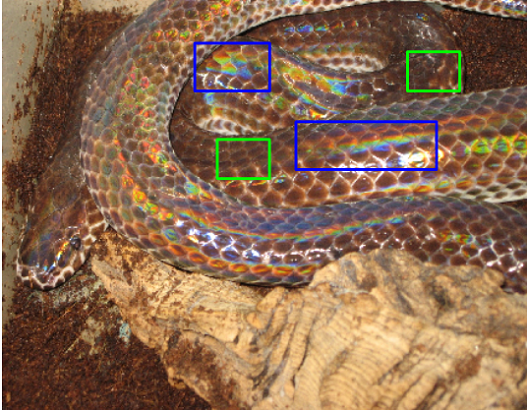
\includegraphics[scale=0.47]{introduction/xenosnake.png}
    \label{fig:xenospeicies}
  }
~
  \subfigure[Elaphe Guttata snake]{
    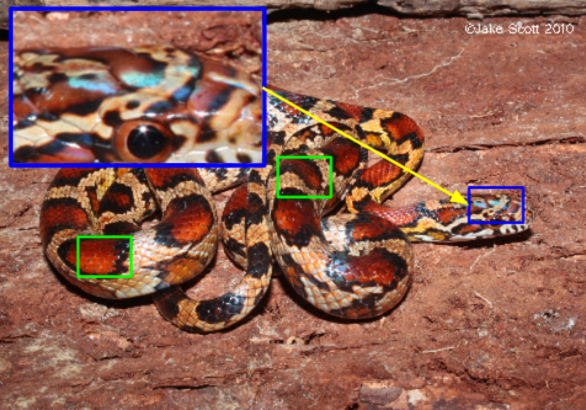
\includegraphics[scale=0.47]{introduction/elaphesnake.png}
    \label{fig:elpahespecies}
  }
  \caption[Example of Biological Color Production]{Examples of pigmentation color (green boxes) and structural color (blue boxes) on different snake species$\footnotemark$.}
  \label{fig:snakespecies}
\end{figure}
\footnotetext{The image source for figure $\ref{fig:xenospeicies}$ is \texttt{http://www.snakes-alive.co.uk/gallery\textunderscore 5.html} and for figure $\ref{fig:elpahespecies}$ is \texttt{http://www.the-livingrainforest.co.uk/living/view\textunderscore price.php?id=464}} 

Some species, like the Xenopeltis, express structural colors in form of iridescent patterns along their scales way stronger than others such as the Elaphe species. The reason lies in the nanostructure of their skins. There are a vast amount of additional reasons for structural color occurrences in nature, such as thin film interference, intra-cellular photonic crystals or diffraction gratings. More detailed examples are shown in figure $\ref{fig:structuralcolorexamples}$. 

\begin{figure}[H]
  \centering
  \subfigure[Thin film interference on a soap bubble]{
    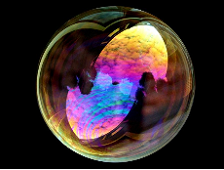
\includegraphics[scale=0.6]{background/soapbubble.png}
    \label{fig:soapbubble}
  }
~
  \subfigure[Multilayer interference on abdomen of a beetle]{
    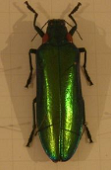
\includegraphics[scale=0.6]{background/beetle.png}
    \label{fig:beetle}
  }
~
  \subfigure[Photonic crystals in the wings of a butterfly]{
    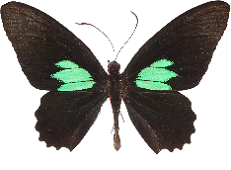
\includegraphics[scale=0.6]{background/butterflypc.png}
    \label{fig:butterflyphotoniccristals}
  }

  \subfigure[Scattering of light from a butterfly's wings]{
    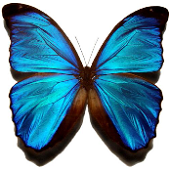
\includegraphics[scale=0.6]{background/butterflyscattering.png}
    \label{fig:butterflyscattering}
  }
~
  \subfigure[Synthetic diffraction grating on a CD]{
    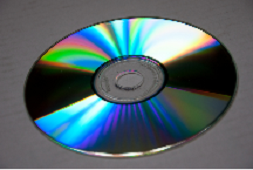
\includegraphics[scale=0.6]{background/cd.png}
    \label{fig:cddiffractiongrating}
  } 
~
  \subfigure[Natural diffraction grating on a snake skin]{
    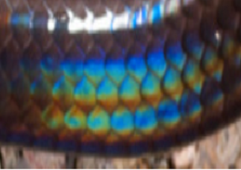
\includegraphics[scale=0.6]{background/snakeskin.png}
    \label{fig:snakediffractiongrating}
  }   
  
  \caption[Structural color examples]{Examples$\footnotemark$ for structural colors on wings and abdomen of insects, liquids, synthetic structures, and on scales on the skin of reptiles.}
  \label{fig:structuralcolorexamples}
\end{figure}
\footnotetext{image source for figures:
\begin{itemize}
  \item \ref{fig:soapbubble}: \texttt{http://www.ualberta.ca/\textasciitilde pogosyan/teaching/PHYS\textunderscore 130/FALL\textunderscore 2010/lectures/lect33/lecture33.html}
  \item \ref{fig:beetle}: \texttt{http://www.itp.uni-hannover.de/\textasciitilde zawischa/ITP/multibeam.html}
  \item \ref{fig:butterflyphotoniccristals}: \texttt{http://upload.wikimedia.org/wikipedia/commons/a/a4/Parides\textunderscore sesostris\textunderscore MHNT\textunderscore dos.jpg}
  \item \ref{fig:butterflyscattering}: From paper \cite{struccolor}, figure 6.
  \item \ref{fig:cddiffractiongrating}: \texttt{http://cnx.org/content/m42496/latest/?collection=col11428/latest}
  \item \ref{fig:snakediffractiongrating}: \texttt{http://www.snakes-alive.co.uk/gallery\textunderscore 5.html}
  \end{itemize}
}

As far back as in the 17th century, Robert Hooke was able to relate the cause of structural colors to the microstructure of a material. During his examinations of peacock feathers, he found that by wetting the feathers, their colors disappeared. Further, he observed that the feathers have tiny ridges. Later, building on top of the knowledge about interference at this times, Newton related structural colors to wave interference. Recently, in the field of computer graphics, many researchers have developed models to render structural colors. Most of these currently available models are not able to perform interactive rendering or are oversimplified and thus cannot accurately model the effects of diffraction from natural gratings. \\

This thesis investigates this particular problem in detail and provides a solution for rendering structural colors that are caused by diffraction on natural gratings at interactive rates.

\section{Goals}
The purpose of this thesis is, to simulate physically accurate structural colors caused by the effect of diffraction on various biological structures and then implement this simulation as a renderer with interactive behaviour. We mainly focus on structural colors generated by natural diffraction gratings. In particular the approach presented in this thesis applies to surfaces with quasiperiodic structures at the nanometer scale, which can be represented as height fields and are visualized as grayscale images. \\

Natural gratings are found on the scale of reptiles, wings of butterflies or the bodies of various insects, but we restrict ourselves and focus on snake skins. The data of our discrete valued height fields, which are representing the surface of a measured snake skin, is acquired using atomic force microscopy (AFM)$\footnote{All data is provided by the Laboratory of Artificial and Natural Evolution in Geneva. See their website:\texttt{www.lanevol.org}}$. Figure $\ref{fig:xenopeltisafm}$ shows a measured height field of a Xenopeltis snake as a grayscale image. The surface of its skin is composed of many finger like structures. Locally, these fingers seem to be very regularly aligned (red box). However, globally, we observe that the alignment of the fingers is curved irregularly (indicated by green curves) along the whole surface. This kind of global irregularity is what makes it hard to model the structural complexity of natural gratings$\footnote{E.g. by relying on statistical methods, caputuring surface details by introducing an appropriate distribution function of the finger strucures.}$.

\begin{figure}[H]
  \centering
  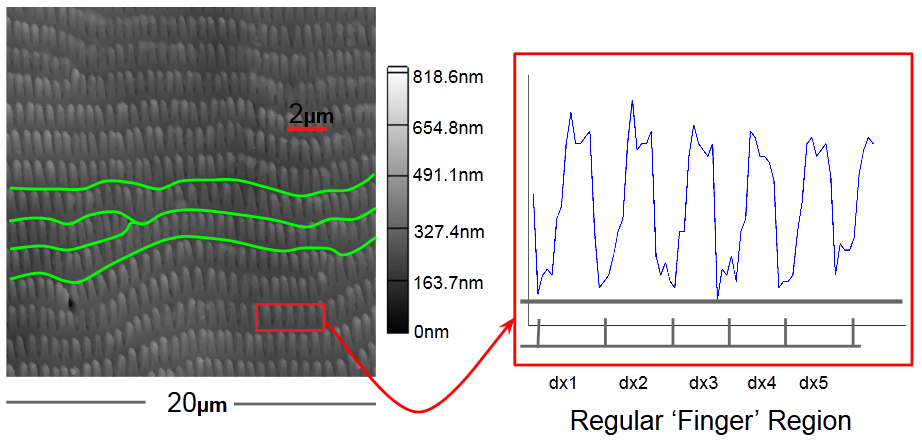
\includegraphics[scale=0.5]{background/samplenaturalgrating.png}
  \caption[Xenopeltis AFM image]{Height field of a Xenopeltis snake$\footnotemark$ skin taken using AFM. Locally, this natural grating consists of regularly aligned (red box) finger-like substructures, but globally we observe a curved alignment of these structures (green curves).}
  \label{fig:xenopeltisafm}
\end{figure}
\footnotetext{This image was provided by the LANE lab in Geneva}

Our renderer established in this thesis is based on the pioneering work of J. Stam about diffraction shaders $\cite{diffstam}$. Stam formulated a BRDF modelling the effect of diffraction based on certain statistical properties of height fields. Nevertheless we have to adapt his BRDF model, since his model assumes that a given surface of a grating can either be formulated by an analytical function and therefore has a closed form solution, or it is modelled effectively by relying on statistical methods. However, we are dealing with natural diffraction gratings (represented as explicitly formulated height fields), which unfortunately are neither known analytically, nor do they fit into simple statistical models. This thesis thus proposes an extension to J. Stam's work for the complex case of explicitly defined, discrete and quasi-periodic height field structures. \\

In the following section a brief overview of relevant previous work and related to this thesis will be presented.

\section{Previous work}
The first scientific descriptions of structural colors were provided by Hooke in 1665 in his book Micrographia$\cite{hookemicro}$. Hooke investigated feathers of peacocks using one of the first microscopes from his time and found out that the colors on the feather were canceled out whenever a drop of water moistened the feather. He proposed the speculation that a layer of thin plates and air were responsible for reflecting the light and thus he related the structure of the feather to colors. In Newton's book Opticks$\cite{newtonopticks}$ he described that the colors of the peacock feather are related to the thinness of the transparent part of the feathers. Around 1800 T.Young explains structural colors as a result of wave interference using his double-slit experiment$\footnote{See \texttt{http://en.wikipedia.org/wiki/Double-slit\textunderscore experiment}}$$\cite{doublslit}$, published in the journal Philosophical Transactions of the Royal Society. \\

In the field of computer graphics, to J.Stam$\cite{diffstam}$ was the first one who was able to develop reflection models based on wave optics capturing the effect of diffraction due to nano-structure height fields. His model is an approximation of far field diffraction$\footnote{See \texttt{http://en.wikipedia.org/wiki/Fraunhofer\textunderscore diffraction}}$ effects relying on the Kirchhof integral$\footnote{See \texttt{http://en.wikipedia.org/wiki/Kirchhoff\textunderscore integral\textunderscore theorem}}$. For a certain class of surfaces which can be modelled as a height field he provides an analytical solution of the BRDF model. He assumes homogeneity of the structure and then the main idea of his model is the formulate a BRDF as the Fourier Transform applied on the the correlation function of the given height field. However, the height fields that Stam is dealing with are either extremely regular or can be considered as a superposition of randomly distributed bumps forming a periodic like structure relying on probabilistic distribution theory$\footnote{See \texttt{http://en.wikipedia.org/wiki/Probability\textunderscore distribution}}$. Both height field assumptions allow him to derive an analytical solution using statistical models. However, the height field we are dealing with are measured, complex, biological nano-structures and thus they do not exhibit regularity at a global scale as demonstrated in figure $\ref{fig:xenopeltisafm}$. It is not sufficient to superimpose one particular nano finger (considering it as a bump) for capturing the complexity of the measured structure since this poses a non-trivial problem of modelling the distribution of nano finger statistically. Therefore, we cannot directly use Stam's BRDF model when we want to perform interactive rendering for diffraction effects of natural gratings.\\

In 2012 Cuypers et all $\cite{reflectancediffmodel}$ proposed a wave based Bidirectional scattering distribution function (BSDF$\footnote{See \texttt{http://en.wikipedia.org/wiki/Bidirectional\textunderscore scattering\textunderscore distribution\textunderscore function}}$) denoted as WBSDF.
Using the rendering equation and Wigner Distribition Functions$\footnote{See \texttt{http://en.wikipedia.org/wiki/Wigner\textunderscore distribution\textunderscore function}}$ (WDF) they related their WBSDF model to the incoming wavefront and hence, their model can be adapted such that it can be rendered by a Monte Carlo renderer. The advantage of their model over Stam's is that their models also captures near field diffraction effects. A disadvantage of their model is that it is computational expensive since the WDF of a two dimensional surface is a four dimensional function and therefore can hardly be used in order to perform interactive rendering. \\

Linday and Agu $\cite{reflectancediffmodel}$ proposed an approach in order to perform interactive rendering diffraction effect by precomputing and storing their BRDF model using spherical harmonics. Nonetheless, for complex natural gratings their BRDF may be insufficient accurate since their approach is using low order spherical harmonics.

\section{Thesis Structure}
The reminder of this thesis is organised as follows: Due to the fact that this thesis has a rather advanced mathematical complexity, chapter 2 introduces some important definitions about modelling light in computer graphics and some wave theory. These concept are required in order to be able to follow our later derivations. This is followed by a brief summary of J. Stam's Paper about diffraction shaders, since his BRDF formulation is the basis of our derivations. \\

In chapter 3 we adapt Stam's BRDF model step-wise in a way that we derive a representation which can be implemented as an interactive diffraction renderer for natural diffraction gratings. We also propose an alternative formulation, which we refer to as the PQ approach in this chapter and discuss its short-comings. \\

Chapter 4 addresses the practical part of this thesis, the implementation of our diffraction model, explaining all precomputation steps and how rendering is preformed in our reference framework for this thesis. \\

Chapter 5 deals with the evaluation of our models. It first provides some insights about diffraction gratings. Then, within this chapter we evaluate the qualitative validity of our BRDF model when applied on different surface gratings by computing their reflectance and comparing the results to the grating equation, under similar conditions. \\

Chapter 6 presents our rendered results, first the BRDF maps for all our gratings and shading approaches under various shading parameters and then the actual renderings on a snake skin. And finally Chapter 7 contains the conclusion of this thesis discussing what has been achieved in this thesis and the drawbacks of the proposed method. It also contains a note about some of my personal experiences during this thesis.

% \newpage{\pagestyle{empty} \cleardoublepage}
% % 
\chapter{Theoretical Background}
\section{Basics in Modeling Light in Computer Graphics}

\subsection{Radiometry}
One purpose of Computer Graphics is to simulate the interaction of light on a surface and how a real-world observer, such as a human eye, will perceive this. These visual sensations of an eye are modeled relying on a virtual camera which captures the emitted light from the surface. The physical basis to measure such reflected light depicts radiometry which is about measuring the electromagnetic radiation transfered from a soruce to a receiver. 

Fundamentally, light is a form of energy propagation, consisting of a large collection of photons, whereat each photon can be considered as a quantum of light that has a position, direction of propagation and a wavelength $\lambda$. A photon travels at a certain speed $v = \frac{c}{n}$, that depends only the speed of light $c$ and the refractive index $n$ through which it progrates. Its frequency is defined by $f = \frac{v}{\lambda}$ and its carried amount of energy $q$, mearsured in the SI unit Joule, is given by $q = hf= \frac{hv}{\lambda n}$ where $h$ is the Plank's constant. The total energy of a large collection of photons is hence $Q = \sum_i q_i$.

\subsection{Spectral Energy}

It is important to understand that the human eye is not equally sensitive to all wavelength of the spectrum of light and therefore responds differently to specific wavelengths. Remember that our goal is to model the human visual perception. This is why we consider the energy distribution of a light spectrum rather than considering the total energry of a photon collection since then we could weight the distribution according the human visual system. So the question we want to answer is: How is the energy distributed across wavelengths of light?

The idea is to make an energy histrogram from a given photon collection. For this we have to order all photons by their associated wavelength, discretize wavelength spectrum, count all photons which then will fall in same wavelength-interval, and then, finally, normalize each interval by the total energy $Q$. This will give us a histogram which tells us the spectral energy $Q_{\lambda}$ for a given discrete $\lambda$ interval and thus models the so called spectral energy distribution $\footnote{Intensive quantities can be thought of as density functions that tell the density of an extensive quantity at an infinitesimal point.}$.

\subsection{Spectral Power}
Rendering an image in Computer Graphics corresponds to capturing the color sensation of an illuminated, target scene at a certain point in time. As previousely seen, each color is associated by a wavelength and is directly related to a certain amount of enegry. In order to determine the color of a to-be-rendered pixel of an image, we have to get a sense of how much light (in terms of energy) passes through the area which the pixel corresponds to. One possibility is to consider the flow of energy $\Phi = \frac{\Delta Q}{\Delta t}$ transferred through this area over a small period of time. This allows us to measure the energy flow through a pixel during a certain amount of time. 

In general, power is the estimated rate of energy production for light sources and corresponds to the flux. It is measured in the unit Watts, denoted by Q. Since power is a rate over time, it is well defined even when energy production is varying over time. As with Spectral Energy for rendering, we are really interested in the spectral power $\Phi_\lambda = \frac{\Phi}{\lambda}$, measured in Watts per nanometer.

\subsection{Spectral Irradiance}
Before we can tell how much light is reflected from a given point on a surface towards the viewing direction of an observer, we first have to know how much light arrives at this point. Since in general a point has no length, area or even volume associated, let us instead consider an infinitimal area $\Delta A$ around a such a point. Then, we can ask ourself how much light falls in such a small area. When further observing this process over a short period in time, this quantity is the spectral irradiance $E$ as illustrated in figure $\ref{fig:irradiance}$. Summarized, this quantity tells us how much spectral power is incident on a surface per unit area and mathematically is equal:

\begin{equation}
 E = \frac{\Phi_{\lambda}}{\Delta A}
\end{equation} 

\begin{figure}[H]
  \centering
  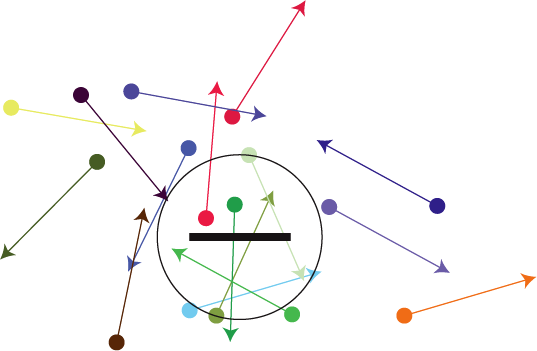
\includegraphics[scale=0.5]{background/irradiance.png}
  \caption{Irradiance is the summed up radiance over all directions}
  \label{fig:irradiance}
\end{figure}

\subsection{Spectral Radiance}
When rendering an image we have to determine the color of each pixel of the image. Although irradiance tells us how much light is arriving at a point as illustrated in figure $\ref{fig:irradiance}$, it tells us little about the direction that light comes from. This relates to how the human eye perceives the brightness of an illuminated objects when looking at it in a certain direction. 

\begin{figure}[H]
  \centering
  \subfigure[Radiances is the density of photons per area per solid angle]{
    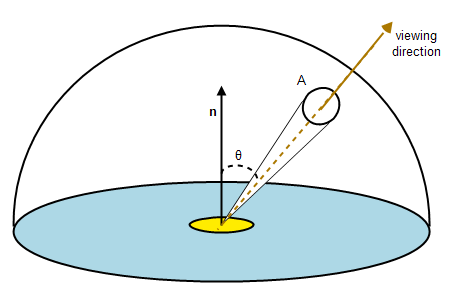
\includegraphics[scale=0.6]{background/radiancehemisphere.png}
    \label{fig:radiance}
  }
~
  \subfigure[Solid angle is the area of a surface patch on a sphere with radius R which is spanned by a set of directions]{  
    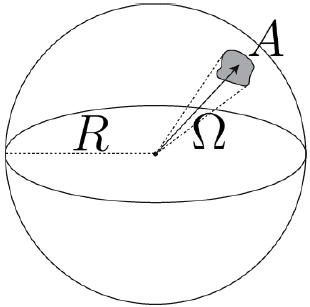
\includegraphics[scale=0.42]{background/solidangle.png}
    \label{fig:solidangle}
  }
  
\label{fig:radianceBasics}
\end{figure}s

This concepted is described by the radiometric quantity radiance. Basically, this is a measure of light energy passing through or is emitted off from a small area around a point on a surface towards a given direction during a short period in time. More formally this is the spectral power emerging from an arbitrary point (an infinitimal area around this point) and falls within a given solid angle (see figure$\footnote{Similar figute like used in computer graphics class 2012 in chapter colors}$ $\ref{fig:solidangle}$)in specific direction (usually towards the observer) as shown in figure $\ref{fig:radiance}$. Formally, this leads us to the following mathematical formalism: 

\begin{equation}
 L_{\lambda}(\omega) = \frac{d^2 \Phi_{\lambda}}{dA d\Omega} \approx \frac{\Phi_{\lambda}}{\Omega A}
\end{equation}

where $L$ is the observed spectral radiance in the unit energy per unit area per solid angle, which is $Wm^-2 sr^-1$ in direction $\omega$ which has an angle $\theta$ between the surface normal and $\omega$, $\Theta$ is the total flux or power emitted, $\theta$ is the angle between the surface normal and the specified direction, $A$ is the area of the surface and $\Omega$ is the solid angle in the unit steradian subtended by the observation or measurement.

It is useful to distinguish between radiance incident at a point on a surface and excitant from that point. Terms for these concepts sometimes used in the graphics literature are surface radiance $L_r$ for the radiance \textit{reflected} from a surface and field radiance $L_i$ for the radiance \textit{incident} at a surface.  

\subsection{BRDF}
In order to render the colorization of an observed object, a natural question in computer graphics is what portion of the reflected, incident light a viewer will receive, when he looks at an illuminated object. Therefore for any given surfaces which is illuminated from a certain direction $\omega_i$, we can ask ourself how much light is reflected off of any point on this surface towards a viewing direction $\omega_r$. This is where the Bidirectional Reflectance Distribution Function (short: BRDF) comes into play, which is a radiometric quantity telling us how much light is reflected at an opaque surface. Mathematically speaking, the BRDF is the ratio of the reflected radiance pointing to the direction $\omega_r$ to the incident irradiance comming from the inverse direction of $\omega_i$ as illustrated in figure $\ref{fig:brdfillustration}$. 

\begin{figure}[ht]
  \centering
  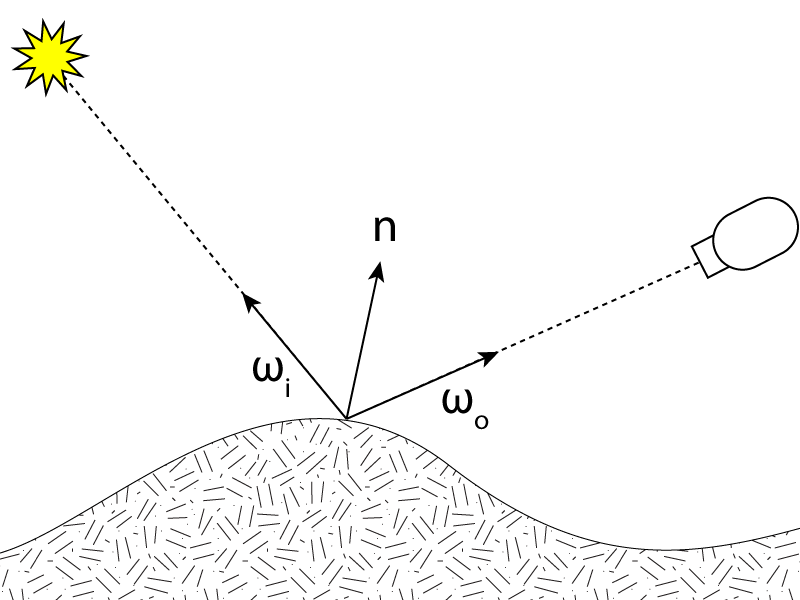
\includegraphics[scale=0.25]{brdfdiagram.png}
  \caption[brdfillustration]{Illistration$\footnotemark$ of the BRDF model, where $\omega_i$ is pointing to the light source and the existing direction is denoted by $\omega_r$. Both direction unit direction vectors defined w.r.t to a surface normal $\mathbf{n}$ for every point on the surface.}
  \label{fig:brdfillustration}  
\end{figure}
\footnotetext{image of illustration has been taken from \href{http://en.wikipedia.org/wiki/Bidirectional_reflectance_distribution_function}{wikipedia}}

Which formally is for any given wavelength $\lambda$ equivalent to:

\begin{align}
  BRDF_{\lambda}(\omega_i, \omega_r)
  & = \frac{dL_r(\omega_r)}{dE_i(\omega_i)} \nonumber \\
  & = \frac{dL_r(\omega_r)}{L_i(\omega_i)cos(\theta_i)d\omega_i}
  \label{eq:defbrdf}
\end{align}

Where $L_{r}$ is the reflected spectral radiance, $E_i$ is the spectral irradiance and $\theta_{\text{i}}$ is the angle between $\omega_{\text{i}}$ and the surface normal $\mathbf n$. 

\subsection{Wavespectrum and Colors}
In order to see how crucial the role of human vision plays, let us consider the following definition of color by \textit{Wyszechkiu and Siles}$\footnote{mentioned in Computer Graphics Fundamentals Book from the year 2000}$ stating that \textit{Color is the aspect of visual perception by which an observer may distinguish differences between two structure-free fields of view of the same size and shape such as may be caused by differences in the spectral composition of the radiant energy concerned in the observation}. Therefore, similarly like the humans' perceived sensation of smell and taste, color vision is just another individual sense of perception giving us the ability to distinguish different frequency distribution of light experienced as color.

\begin{figure}[H]
  \centering
  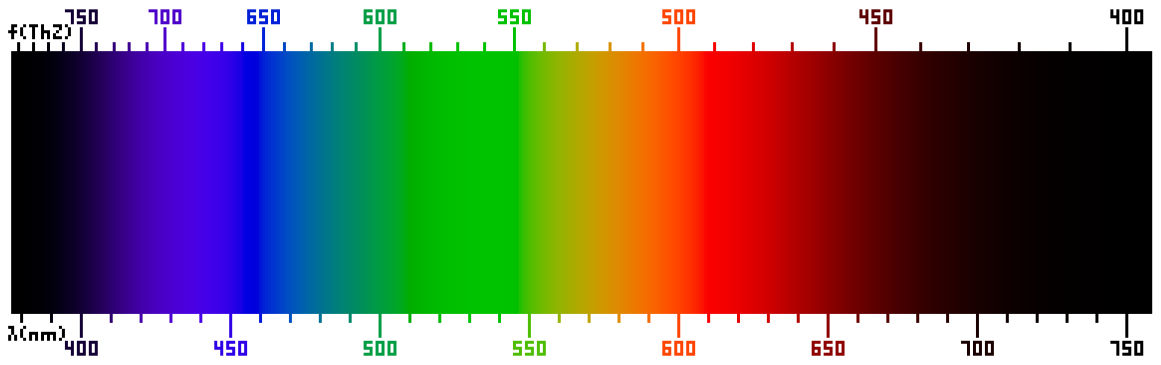
\includegraphics[scale=0.35]{background/lightspec.png}
  \caption[visiblelightspectrum]{Frequency (top) and wavelenght (bottom) of colors of the visible light spectrum$\footnotemark$.}
  \label{fig:colorspectrum}
\end{figure}
\footnotetext{Similar figute like used in computer graphics class 2012 in chapter colors}

In general an eye consists of photoreceptor cells which are responsible for providing ability of color-perception. A schematic of an eye is illustratied in figure $\ref{fig:humaneye}$. Basically, there are two specialized types of photoreceptor cells, cone cells which are responsible for color vision and rod cells, which allow an eye to perceive different brigthness levels.

\begin{figure}[H]
  \centering
  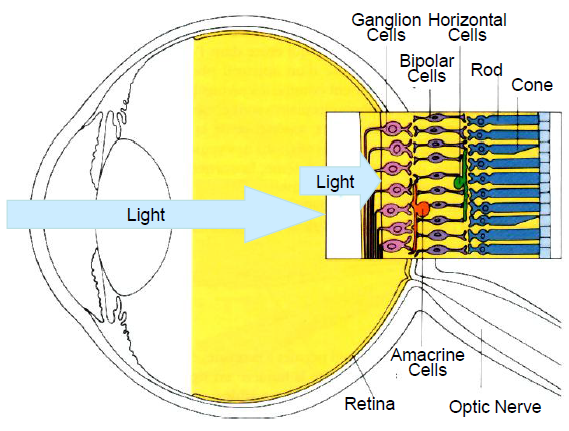
\includegraphics[scale=0.35]{background/humaneye.png}
  \caption[humanayeschematic]{Schematic$\footnotemark$ of photoreceptor cells, cones and rods, in human eye }
  \label{fig:humaneye}
\end{figure}
\footnotetext{image of illustration has been taken from \href{http://en.wikipedia.org/wiki/Bidirectional_reflectance_distribution_function}{wikipedia}}

A human eye is made of three different types of cone cells, having their peak sensivity in sensing color at different wavelength ranges. More precisely, there are cone cells most sensitive to short wavelengths which are between $420 nm$ and $440 nm$, those which are most sensitive in the middle range between $530 nm$ and $550 nm$ and those which have their peak in the long range, from $560 nm$ to $580 nm$. In principle, any color sensation in human color perception as shown in figure $\ref{fig:colorspectrum}$ can therefore be described by just three parameters, corresponding to levels of stimulus of the three types of cone cells.  

\subsection{Colorspace}
In order to render accurately images of how a human observer sees its world, a mathematical model of the human color perception is required. Remember that color sensation is due to a visual stimulus processed by cone cells in an eye. A human eye contains three different types of cone cells. Therefore, one possible approach is to describe each kind of these cone cells as a function of wavelength, returning a certain intensivity. In the early 1920, from a series of experiments the so called CIE XYZ color space was derived, describing response of cone cells of an average human individual, the so called standard observer. Basically, a statistically sufficiently large number of probands were exposed to different target light colors expressed by their wavelength. The task of each proband was to reproduce these target colors by mixing three given primary colors, red-, green- and blue-light. The strength  of each primary color could be manually adjusted by setting their relative intensivity. Those adjustment weights have been measured, aggregated and averaged among all probands for each primary color. This model describes each color as a triple of three real valued numbers$\footnote{note that there are  negative color weights possible in the CIE XYZ colors space. This is why some human perceived color sensations could not be reconstructed using just an additive color model (adding three positively weighted primary values). Therefore, a probabant was also allowed to move one of the primary colors to the target color and instead was supposed to reproduce this new color mix using the two remaining primaries (subtractive model). The value of the selected, moved primary was then interpreted as beeing negative weighted in an additive color model.}$, the so called tristimulus values.

Pragmatically speaking, color spaces describes the range of colors a camera can see, a printer can print or a monitor can display. Thus, formally we can define it as a mapping a range of physically produced colors from mixed light to an objective description of color
sensations registered in the eye of an observer in terms of tristimulus values. 

\begin{figure}[H]
  \centering
  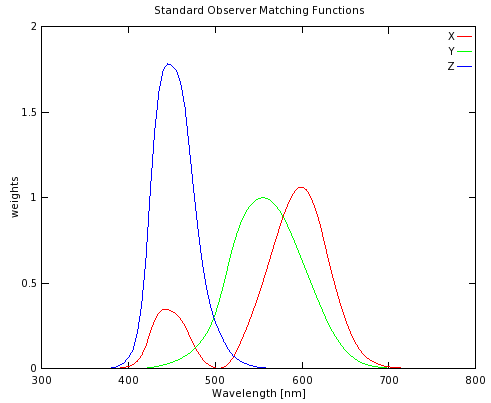
\includegraphics[scale=0.7]{background/somatchingfunctions.png}
  \caption{Plots of our color matching functions we used for rendering}
  \label{fig:matchingfunction}
\end{figure}

Interpolating all measured tristimuli values gives us three basis functions, the CIE color matching functions $\overline{x}(\lambda)$, $\overline{y}(\lambda)$, $\overline{z}(\lambda)$. In figure $\ref{fig:matchingfunction}$ are the numerical description of the chromatic response of the observer. They can be thought of as the spectral sensitivity curves of three linear light detectors yielding the CIE Tristimulus values X, Y and Z. 

The tristimulus values for a color with a spectral power distribution $I(\lambda)$, are given in terms of the standard observer by:

\begin{align}
    X= \int_{\Lambda} I(\lambda)\,\overline{x}(\lambda)\,d\lambda \nonumber \\
    Y= \int_{\Lambda} I(\lambda)\,\overline{y}(\lambda)\,d\lambda \nonumber \\
    Z= \int_{\Lambda} I(\lambda)\,\overline{z}(\lambda)\,d\lambda
\label{eq:tristimulusvalues}
\end{align}

Where $\lambda$, is the wavelength of the equivalent monochromatic light spectrum $\Lambda = [380nm, 780nm]$. Note taht it is not possible to build a display that corresponds to the CIE XYZ colorspace. For this reasons it is necessary to design other color spaces, which are physical realizable, offers efficient encoding, are perceptual uniform and have an intuitive color specification. There are simple conversions between XYZ color space, to other color space described as linear transformations.

\subsection{Spectral Rendering}
When rendering an image, most of the time we are using colors described in a certain RGB color space. However, a RGB colorspace results from a colorspace transformation of the tristimulus values, which themself are inherent to the human visual system. Therefore, many physically light phenomenon are poorly modeled when always relying on RGB colors for rendering. Using only RGB colors for rendering is alike we would assume that a given light source emits light of only one particular wavelength. But in reality this is barely the case. Spectral rendering is referring to use a certain wavelength spectrum, e.g. the human visible light spectrum, instead simply using the whole range of RGB values in order to render an illuminated scene. This captures the physical reality of specific light sources way more accurate. Keep in mind that, even when we make use of a spectral rendering approach, we have to convert the final spectra to RGB values, when we want to display an image on an actual display. 

\section{Wave Theory for Light and Diffraction}
\subsection{Basics in Wave Theory}
In order prepare the reader for physical relevant concepts used during later derivations and reasonings within this thesis, I am going to provide a quick introducation to the fundamental basics of wave theory and related concepts. In physics a wave describes a disturbance that travels from one location to another through a certain medium. The disturbance temporarly displaces the particles in the medium from their rest position which results in an energy transport along the medium during wave propagation. Usually, when talking about waves we are actually refering to a complex valued function which is a solution to the so called wave equation which is modeling how the wave disturbance proceeds in space during time. 

There are two types of waves, mechanical waves which deform their mediums during propagation like sound waves and electromagnetic waves consiting of periodic oscilations of an electromagnetic field such as light for example. Like simplified illustrated in figure $\ref{fig:wavebasics}$, there are several properties someone can use and apply in order to compare and distinguish different waves:

\begin{figure}[H]
  \centering
  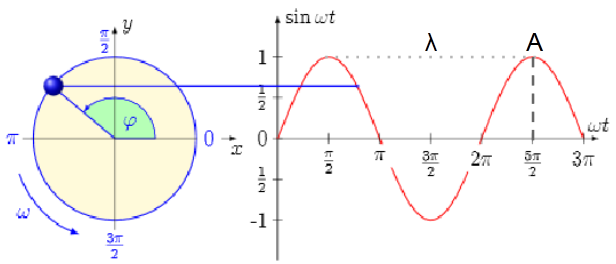
\includegraphics[scale=0.65]{background/waveschematicimpr.png}
  \caption[sinewave]{Simplified, one dimensionaly real valued wave function$\footnotemark$, giving an idea about some important wave properties. We denote the crest of a wave as the hightest point relative to the equilibrium line (zero height along time axis) and similarly the trough as the lowest point.}
  \label{fig:wavebasics}
\end{figure}
\footnotetext{Image source: http://neutrino.ethz.ch/Vorlesung/FS2013/index.php/vorlesungsskript}

\begin{description}
  \item[Wavelength:] Is usually denoted by $\lambda$ and is a measure for the spatial distance from one point to another until the shape of a wave repeats
  \item[Amplitude:] Is denoted by $A$ and there are two possible interprations: First, it is a measure of the height from the equilibrium point to the heighest point of a crest on the wave or the lowest point of a trough. This mean the amplitude can be positive or negative. However, usually, someone is  just interested the absolute value of an amplitude, the magnitude of a wave. For light waves it is a relative measure of intensity or brightnes to other lught waves of the same wavelength. And secondly, it can be interpreted as a measure how much energy a wave carries wherate the greater the absoulte aplitute value, the bigger the amount of energy being carried.
  \item[Frequency:] Is a measure of the number of waves which are passing through a particular point in the propagation medium during a certain time and is denoted by $f$.
  \item[Phase:] Is denoted by $\phi$. Describes either the offset of initial position of a wave or the relative displacement between or among waves having the same frequency. Two waves two waves with same frequency are denoted by being in phase if they have the same phase. This means they line up everywhere. As a remark, we denote by $\omega$ the angular frequency which is equal $2\pi f$. 
\end{description}

A geometrical property of waves is their wavefront. This is either a surface or line along the path of wave propagation on which the disturbance at every point has the same phase. Three are basically three types of wavefronts: spherical-, cylindrical- and plane wavefront. If point in a isotropic medium is sending out waves in three dimensions, then the coresponding wavefronts are spheres, centered on the source point. Hence spherical wavefront is the result of a spherical wave, also denoted as a wavelet. Note that for electromagnetic waves, the phase is a poisition of a point in time on a wavefront cycle (motion of wave over a whole wavelength) whereat a complete cycle is defined as being equal 360 degrees.



\subsection{Wave Interference}
Next, after having seen that a wave is simply a traveling disturbance along a medium, having some special properties, someone could ask what happens when there are several waves travaling on the same medium. Especially, we are interested how these waves will interac with each other. In physics we use the term interference for the resulting phenomenon when two or more waves meet. Hence interference is the interaction of waves when they encounter each other at a point along their medium of propagation. At each point where two waves superpose, their total displacement at these points is the sum of the displacements of each indiviudal wave at those points. Then, the resulting wave is having a greater or lower amplitude than each seperate wave and this we can interprete the interference as the addition operator for waves. Two extreme scenarios are illustrated in figure $\ref{fig:interferenceconcept}$. There are basically three variants of interferences which can occur, depending on how crest and troughs of the waves are matched up:

\begin{figure}[H]
  \centering
  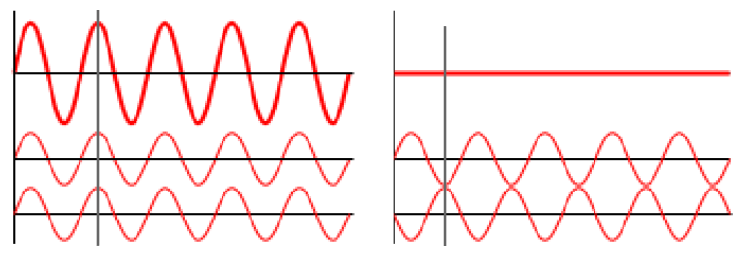
\includegraphics[scale=0.65]{background/interferenceconcept.png}
  \caption[interference]{Interference scenarios$\footnotemark$ when two waves waves meet: On the left handside, there is constructive interference and on the right handside there is destructive interference illustrated.}
  \label{fig:interferenceconcept}
\end{figure}
\footnotetext{Image source: \texttt{http://en.wikipedia.org/wiki/Interference\textunderscore(wave\textunderscore propagation)} } 

\begin{itemize}
  \item Either a crest of a wave meets a crest of another wave or similarly a trough meets a trough of another wave. This scenario is denoted as constructive interference and occurs at any location along the medium where the two interfering waves have a displacement in the same direction. This is equivalent like saying that the phase difference between the waves is a multiple of $2\pi$. Then the resulting amplitude at that point is being much larger than the amplitude of an individual wave. For two waves with an equal amplitude interfering constructively, the resulting amplitude is twice as large as the amplitude of an individual wave.
  \item Either a crest of a wave meets a trough of another wave or vice versa. This scenario is denoted as destructive interference and occurs at any location along the medium where the two interfering waves have a displacement in the opposite direction. This is like saying that the phase difference between the waves is an odd multiple of $\pi$. Then the waves completely cancel each other out at any point they superimpose.
  \item If the phase difference between two waves is intermediate between the first two scenarios, then the magnitude of the displacement lies between the minimal and maximal values which we could get from constructive interference.
\end{itemize}

\subsection{Wave Coherence}
\subsubsection{Concept of Coherence}
When considering waves which are traveling on a shared medium along the same direction, we could examine how their phase difference is changing over time. Formulating the changement of their relative phase as a function of time will provides us a quantitative measure of the synchronism of two waves, the so called wave coherence. In order to better understand this concept, let us consider a perfectly mathematical sine wave and second wave which is a phase-shifted replica of the first one. A property of mathematical waves is that they keep their shape over an infinity amount of moved wavelengths. In our scenario, both waves are traveling along the same direction on the same medium, like exemplarily illustrated in figure $\ref{fig:coherencesinsignal}$.
\begin{figure}[H]
  \centering
  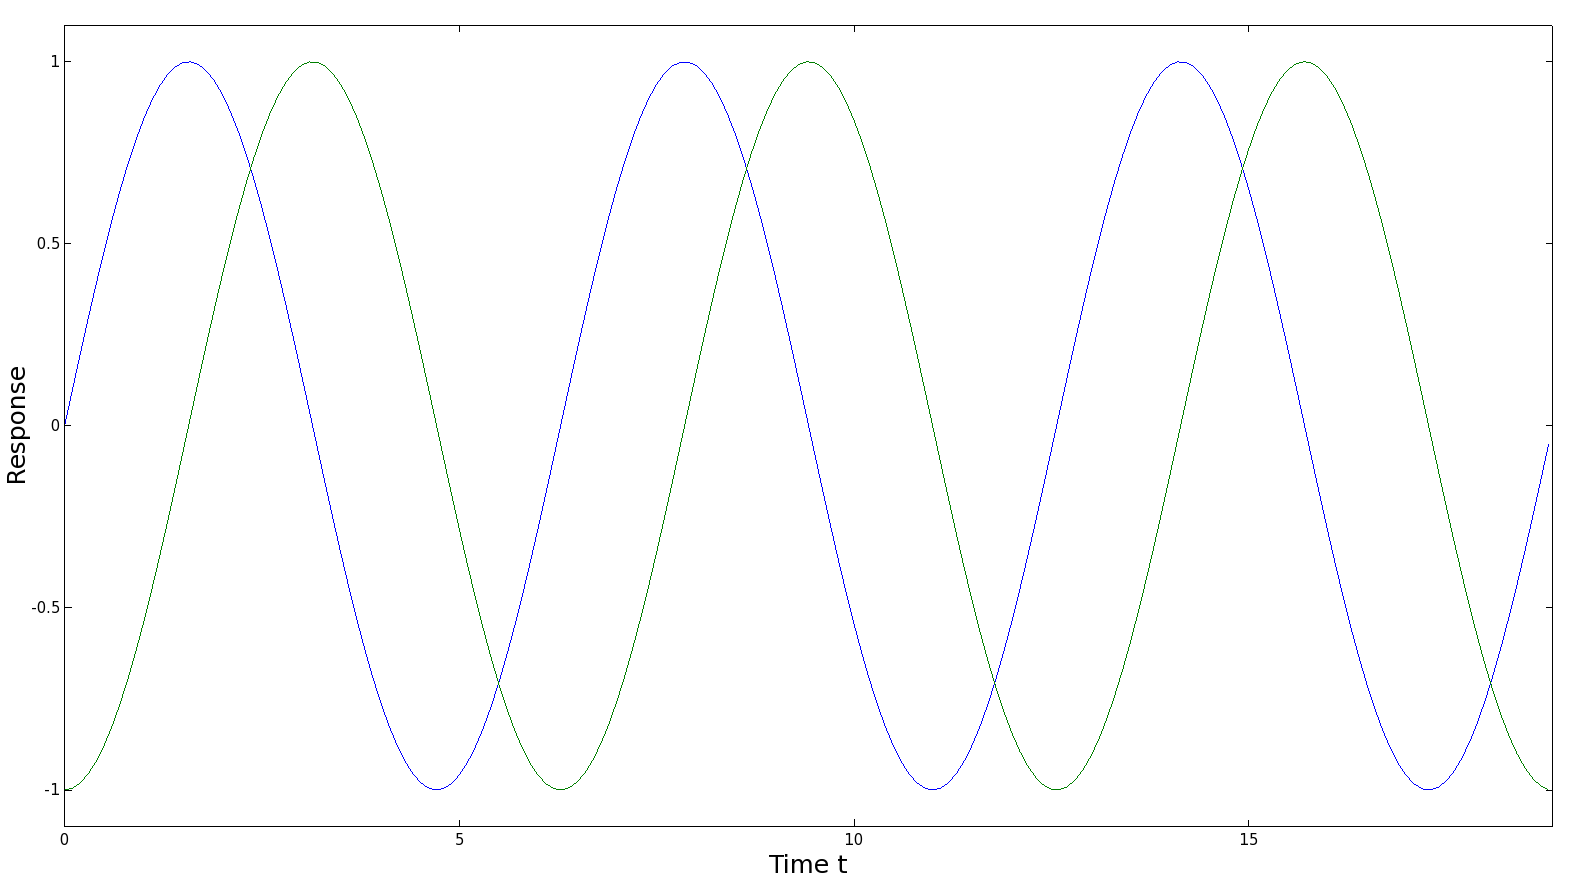
\includegraphics[scale=0.3]{background/coherencesinsignal.png}
  \caption{Two mathematical sine waves which are perfectly coherent which means that their phase difference is constant for every point in time.}
  \label{fig:coherencesinsignal}
\end{figure}

Taking the difference between the two sine waves from the previous figure yields always a constant number. Therefore, those two waves are said to be coherent and hence perfectly synchronous over time. Notice that this scenario is completly artificial since in nature there are no mathematical sine waves. Rather, the phase difference is then a fuction of time $p(t)$. The more coherent two waves are, the slower this function will change over time. 
In fact, two waves are said to be coherent if they are either of the same frequency, temporally in phase or have the same amplitude at every point in time.
Thus two waves are coherent if they are generated at the same time, having the same frequency, amplitude, and phase. Reversely, Waves are considered incoherent or also asynchronous if they have no stable phase difference. This means $p(t)$ is heavly varying over time. Coherence describes the effect of whether waves will tend to interfere with each other constructively or destructively at a certain point in time and space. Thus this is a property of waves that enables stationary interference. The more correlated two waves are, the higher their degree of coherence is. In physics coherence between waves is quantified by the corss-correlation function, which basically predicts the value of a second wave using the value of the first one. There are two basic coherence classifications:

\begin{itemize}
  \item Spatial coherence is dealing with the question of what is the range of distance between two points in space in the extend of a wave for which there is occuring a significant effect of interference when averaged over time. This is formally answered by considering the correlation between waves at different point in space. The range of distance is also denoted as the coherence area.
  \item Temporal coherence examines the ability of how well a wave will interfer with itself at different moments in time. Mathematically, this kind of coherence is computed by averaging the measured correlation between the value of the wave and the delayed version of itself at different pairs of time. The Coherence time denotes the time for which the propagating wave is coherent and we therefore can predict its phase using the correlation function. The distance a wave has traveled during the coherence time is denoted as the coherence length.
\end{itemize}

\subsubsection{Derivation}
inject contribution here

\subsection{Huygen's Principle}
\subsection{Waves Diffraction}


\section{Stam's BRDF formulation}
\label{sec:sumstam}
In his paper about Diffraction Shader, J. Stam derives a BRDF which is modeling the effect of diffraction for various analytical anisotropic reflexion models relying on the so called scalar wave theory of diffraction for which a wave is assumed to be a complex valued scalar. 
It's noteworthy, that Stam's BRDF formulation does not take into account the polarization of the light. Fortunately, light sources like sunlight and light bulbs are unpolarized. 

A further assumption in Stam's Paper is, the emanated waves from the source are stationary, which implies the wave is a superposition of independent monochromatic waves. This implies that each wave is associated to a definite wavelength lambda. However, sunlight once again fulfills this fact.

In our simulations we will always assume we have given a directional light source, i.e. sunlight. Hence, Stam's model can be used for our derivations.

For his derivations Stam uses the Kirchhoff integral (ADD REF TO WIKI), which is relating the reflected field to the incoming field. This equation is a formalization of Huygen’s well-known principle that states that if one knows the wavefront at a given moment, the wave at a later time can be deduced by considering each point on the first wave as the source of a new disturbance. Mathematically speaking, once the field  $\psi_1 =  e^{ik\mathbf{x} \cdot \mathbf{s}\mathbf{s}}$ on the surface is known, the field $\psi_2$ everywhere else away from the surface can be computed.
More precisely, we want to compute the wave $\psi_2$ equal to the reflection of an incoming planar monochromatic wave $\psi_1 = e^{ik \omega_i * x}$  traveling in the direction $\omega_i$ from a surface $S$ to the light source. Formally, this can be written as:

\begin{equation}
\psi_{2}(\omega_i, \omega_r) = \frac{i k e^{i K R}}{4 \pi R} (F(-\omega_i-\omega_r)-(-\omega_i+\omega_r)) \cdot I_{1}(\omega_i, \omega_r) 
\label{eq:kirchhoff}
\end{equation}

with

\begin{equation}
I_{1}(\omega_i, \omega_r) = \int_{S} \hat{\mathbf{n}} e^{ik(-\omega_i-\omega_{r}) \cdot \mathbf{s} d\mathbf{s}}
\label{eq:IBase}
\end{equation}

In applied optics, when dealing with scattered waves, one does use differential scattering cross-section rather than defining a BRDF which has the following identity: 

\begin{equation}
    \sigma^0 = 4 \pi \lim_{R \to \infty} R^2 \frac{\langle \left|\psi_2\right|^2\rangle}{\langle \left|\psi_1\right|^2\rangle}
\end{equation}

where R is the distance from the center of the patch to the receiving point $x_p$, $\hat{\mathbf{n}}$ is the normal of the surface at s and the vectors:

The relationship between the BRDF and the scattering cross section can be shown to be equal to 

\begin{equation}
 BRDF = \frac{1}{4\pi}\frac{1}{A}\frac{\sigma^0}{cos(\theta_i)cos(\theta_r)}
 \label{fig:crossscateringbrdfrelationship} 
\end{equation}

where $\theta_i$ and $\theta_r$ are the angles of incident and reflected directions on the surface with the surface normal $n$. See ~\ref{fig:geometricsetup}.

\begin{figure}[ht]
  \centering
  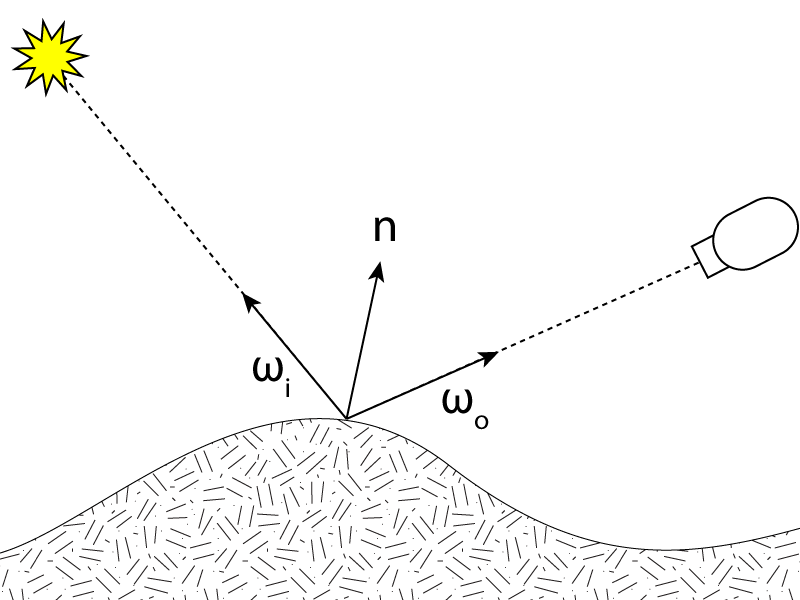
\includegraphics[scale=0.25]{brdfdiagram.png}
  \caption{$\omega_i$ points toward the light source, $\omega_r$ points toward the camera, $n$ is the surface normal}
  \label{fig:geometricsetup}  
\end{figure}

The components of vector resulting by the difference between these direction vectors:
In order to simplify the calculations involved in his vectorized integral equations, Stam considers the components of vector 
\begin{equation}
  (u,v,w) = -\omega_i - \omega_r 
\label{eq:uvw}
\end{equation}

explicitly and introduces the equation: 
\begin{equation}
  I(ku,kv) = \int_{S} \hat{\mathbf{n}} e^{ik(u,v,w) \cdot \mathbf{s} d\mathbf{s}} 
\label{eq:Istart}
\end{equation}

which is a first simplification of $\ref{eq:IBase}$. Note that the scalar $w$ is the third component of ~\ref{eq:uvw} and can be written as $w = -(cos(\theta_i)+cos(\theta_r))$ using spherical coordinates. The scalar $k=\frac{2\pi}{\lambda}$ represent the wavenumber.


During his derivations, Stam provides a analytical representation for the Kirchhoff integral assuming that each surface point $s(x,y)$ can be parameterized by $(x,y,h(x,y))$ where $h$ is the height at the position $(x,y)$ on the given $(x,y)$ surface plane. Using the tangent plane approximation for the parameterized surface and plugging it into $\ref{eq:Istart}$ he will end up with: 

\begin{equation}
    \mathbf{I}(ku, kv) = \int \int (-h_{x}(x,y), -h_{y}(x,y), 1) e^{ikwh(x,y)} e^{ik(ux + vy)} dx dy
\label{eq:I1}
\end{equation}

For further simplification Stam formulates auxillary function which depends on the provided height field: 
\begin{equation}
  p(x,y) = e^{iwkh(x,y)} 
\label{eq:px}
\end{equation}

which will allow him to further simplify his equation $\ref{eq:I1}$ to:

\begin{equation}
    \mathbf{I}(ku, kv) = \int \int \frac{1}{ikw}(-p_x, -p_y, ikwp) dx dy
\label{eq:I2}
\end{equation}

where he used that $(-h_{x}(x,y), -h_{y}(x,y), 1)e^{kwh(x,y)}$ is equal to $\frac{(-p_x, -p_y, ikwp)}{ikw}$ using the definition of the partial derivatives applied to the function $\ref{eq:px}$.

Let $P(x,y)$ denote the Fourier Transform (FT) of $p(x,y)$. Then, the differentiation with respect to x respectively to y in the Fourier domain is equivalent to a multiplication of the Fourier transform by $-iku$ or $-ikv$ respectively. This leads him to the following simplification for $\ref{eq:I1}$:

\begin{equation}
    \mathbf{I}(ku, kv) = \frac{1}{w}P(ku, kv) \cdot (u,v,w)
\label{eq:I3}
\end{equation}

Let us consider the term $g = (F(-\omega_i - \omega_r)-(-\omega_i + \omega_r))$, which is a scalar factor of $\ref{eq:kirchhoff}$. The dot product with $g$ and $(-\omega_i - \omega_r)$ is equal $2F(1 + \omega_i \cdot \omega_r)$. Putting this finding and the identity $\ref{eq:I3}$ into $\ref{eq:kirchhoff}$ he will end up with:

\begin{equation}
\psi_{2}(\omega_i, \omega_r) = \frac{i k e^{i K R}}{4 \pi R} \frac{2F(1 + \omega_i \cdot \omega_r)}{w} P(ku, kv)
\label{eq:kirchhoffFinding}
\end{equation}

By using the identity $\ref{fig:crossscateringbrdfrelationship}$, this will lead us to his main finding:
\begin{equation} 
  BRDF_{\lambda}(\omega_i, \omega_r) = \frac{k^2 F^2 G}{4\pi^2 A w^2} \langle \left|P(ku, kv)\right|^2\rangle
\label{eq:mainstam}
\end{equation}

where $G$ is the so called geometry term which is equal: 

\begin{equation}
  G =\frac{(1 + \omega_i \cdot \omega_r)^2}{cos(\theta_i)cos(\theta_r)}
\label{eq:geometricterm}
\end{equation}


\newpage{\pagestyle{empty} \cleardoublepage}
% % % 
\chapter{Derivations}
\label{chap:derivations}

\section{Problem Statement and Challenges}
The goal of this thesis is to perform a physically accurate and interactive simulation of structural colors production like shown in figure $\ref{fig:problemstatementoutput}$, which we can see whenever a light source is diffracted on a natural grating. For this purpose we need to be provided by the following input data as shown in figure $\ref{fig:problemstatement}$:
\begin{itemize}
  \item A mesh representing a snake surface$\footnote{Which is in our simulation an actual reconstruction of a real snake skin. These measurements are provided by the Laboratory of Artificial and Natural Evolition at Geneva.See their website:\texttt{www.lanevol.org}.}$ with associated texture coordinates as shown in figure $\ref{fig:strucgeom}$.
  \item A natural diffraction grating represented as a height field, its maximum height and its pixel-width-correspondence$\footnote{Since the nanostructure is stored as a grayscale image, we need a scale telling us what length and height one pixel cooresponds to in this provided image.}$.
  \item A vectorfield which describes how fingers on a provided surface of the nanostructrue are aligned as shown in figure $\ref{fig:patchvectorfield}$. 
\end{itemize}

\begin{figure}[H]
  \centering
  \subfigure[Structure Geometry]{
    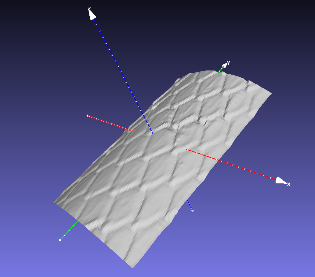
\includegraphics[scale=0.40]{derivation/structuregeom.png}
    \label{fig:strucgeom}
  }
~
  \subfigure[Nanostructure Surface]{
    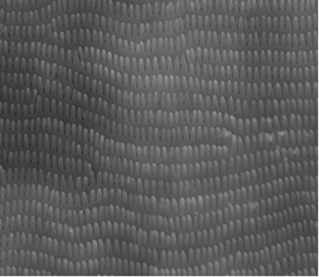
\includegraphics[scale=0.40]{derivation/nanostructuresurface.png}
    \label{fig:nanostruc}
  }
~
  \subfigure[Patch Orientation]{
    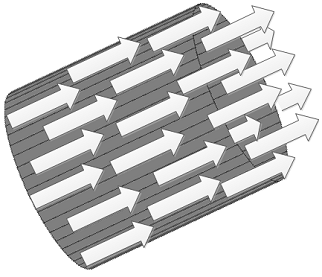
\includegraphics[scale=0.40]{derivation/vectorfieldalongcylinder.png}
    \label{fig:patchvectorfield}
  }
  \caption[Problem Statement]{Input for our simulation}
  \label{fig:problemstatement}
\end{figure}

We want to rely on the integral equation $\ref{eq:mainstam}$ derived by J. Stam in his paper $\cite{diffstam}$ about diffraction shaders. This equation formualtes a BRDF modeling the effect of diffraction under the assumption that a given grating can either be formulated as an analytical function or its structure is simple enough beeing modeled relying on statistical methods. These assumptions guarantee that $\ref{eq:mainstam}$ has an explicit solution. However, the complexisty of a biological nanostructures cannot sufficiently and accurately modeled simply using statistical methods. This is why interactive computation at high resolution becomes a hard task, since we cannot evaluate the given integral equation on the fly. Therefore, we have to adapt Stam's equation such that we are able to perform interactive rendering using explicitly provided height fields.

\begin{figure}[H]
  \centering
  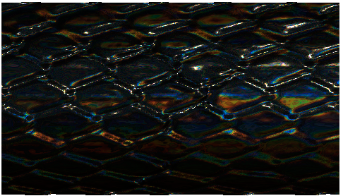
\includegraphics[scale=0.5]{derivation/renderedstructuredcolors.png}
  \caption[Problem Statement: Output]{Output: Rendered Structural Colors}
  \label{fig:problemstatementoutput}
\end{figure}


\section{Approximate a FT by a DFT}
\subsection{Reproduce FT by DTFT}
In the previous section, we have found an identity for the reflected spectral radiance $L_{\lambda}(\omega_r)$ when using Stam's BRDF for a given input height field. However, the derived expression in equation $\ref{eq:nonrelativebrdffinding}$ requires to evaluate the Fourier Transform of our height field$\footnote{actually it requires the computation of the inverse Fourier Transform of a transformed version of the given heightfield, the function p(x,y) defined in equation \ref{eq:px}.}$ for every direction. In this section we explain how to approximate the FT by the DTFT and apply it to our previous derivations. Figure $\ref{fig:ftbydtft}$ graphically shows how to obtain the DTFT from the FT for a one dimensional signal$\footnote{For our case we are dealing with a two dimensional, spatial signal, the given height field. Nevertheless, without any constraints of generality, the explained approach applies to multi dimensional problems.}$ \\

\begin{figure}[ht]
  \centering
  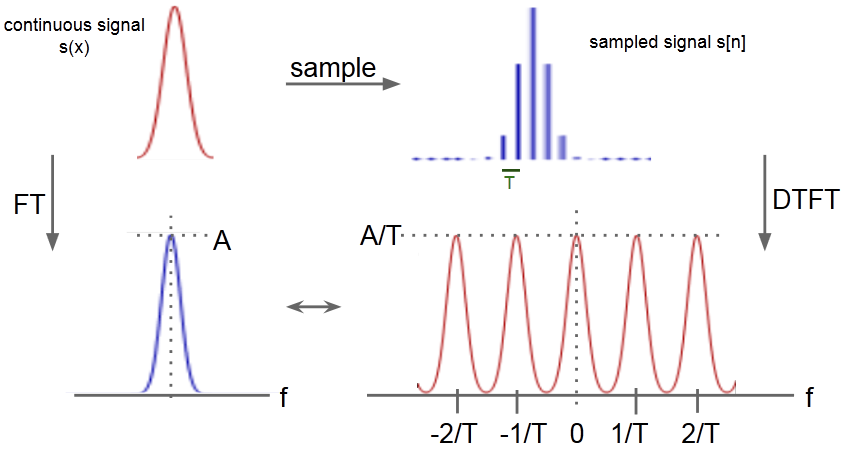
\includegraphics[scale=0.6]{derivation/ftbydtft.png}
  \caption[FT by DTFT]{Illustration of how to approximate the analytical Fourier Transform (FT) $\footnotemark$ of a given continuous signal by a Discrete Time Fourier Transform (DTFT). The DTFT applied on a bandlimited, discretized signal yields a continuous, periodic response in frequency space.}
  \label{fig:ftbydtft}  
\end{figure}
\footnotetext{Images of function plots taken from \texttt{http://en.wikipedia.org/wiki/Discrete\textunderscore Fourier\textunderscore transform} and are modified.} 
The first step is to uniformly discretize the given signal since computers are working finite, discrete arithmetic. We rely on the Nyquist–Shannon sampling theorem tells us how dense we have to sample a given signal $s(x)$ such that can be reconstructed its sampled version $\hat{s}[n]$$\footnote{n denotes the number of samples.}$. In particular, a sampled version according to the Nyquist–Shannon sampling theorem will have the same Fourier Transform as its origianl singal. The sampling theorem states that if $f_{max}$ denotes the highest frequency of $s(x)$, then, it has to be sampled by a rate of $f_s$ with $2f_{max} \leq f_s$ in order to be reconstructable. By convention $T = \frac{1}{f_s}$ represent the interval length between two samples. \\ \\

Next, we apply the Fourier Tranformation operator on the discretized singal $\hat{s}$ which gives us the following expression: 

\begin{align}
\mathcal{F}_{FT}\{\hat{s}\}(w)
& = \int_{\mathds{R}} \hat{s}[n] e^{-iwx} dx \nonumber\\
& = \int_{\mathds{R}} mask(x)s(x) e^{-iwx} dx \nonumber\\
& = T\sum_{x=-\infty}^{\infty} \hat{s}[x] e^{-iwx} \nonumber\\
& = T\mathcal{F}_{DTFT}\{s\}(w)
\label{eq:sampledsignalfttodtft}
\end{align} 
Equation $\ref{eq:sampledsignalfttodtft}$ tells us that if $\hat{s}$ is sufficiently sampled, then its DTFT corresponds to the FT of $s(x)$ . Notice that the resulting DTFT from the sampled signal has a height of $\frac{A}{T}$ where A is the height of the FT of $s$ and thus is a scaled version of the FT. \\

For a given height field $h$, let us compute Stam's auxiliary function $p$ defined as in equation $\ref{eq:px}$. For the reminder of this thesis we introduce the following definition: 

\begin{equation}
  P_{dtft} \equiv \mathcal{F}_{DTFT}\{p\}
\label{eq:dtftheightfield}
\end{equation} 

Therefore $P_{dtft}$ denotes the DTFT of a transformed version of our height field $h$$\footnote{By transformed height field we mean $p(x,y) = e^{i\frac{2 \pi}{\lambda} w h(x,y)} which we get, when pluggin $h$ into equation \ref{eq:heightfieldphase} and this expression again plug into equation \ref{eq:px}.$}$. 

\subsection{Spatial Coherence and Windowing}
\label{sec:spatialcoherenceandwindowing}
Before we can derive a final expression in order to approximate a FT by a DFT, we first have to revisit the concept of coherence introduced in section $\ref{sec:wavecoherence}$ of chapter 2.Previousely we have seen that Stam's BRDf tells us what is the total contribution of all secondary sources which allows us to say what is the reflected spectral radiance at a certain point in space. This is related to stationary interference which itself depends on the coherence property of the emitted secondary wave sources. The ability for two points in space, $t_1$ and $t_2$, to interfere in the extend of a wave when being averages over time is the so called spatial coherence. The spatial distance between such two points over which there is significant intererence is limited by the quantity coherence area. For filtered sunlight on earth this is equal to 65$\mu m$ $\footnote{A proof for this number can be looked up in the book Optical Coherence and Quantum Optics$\cite{optcoherence}$ on page 153 and 154.}$.

\begin{figure}[H]
  \centering
  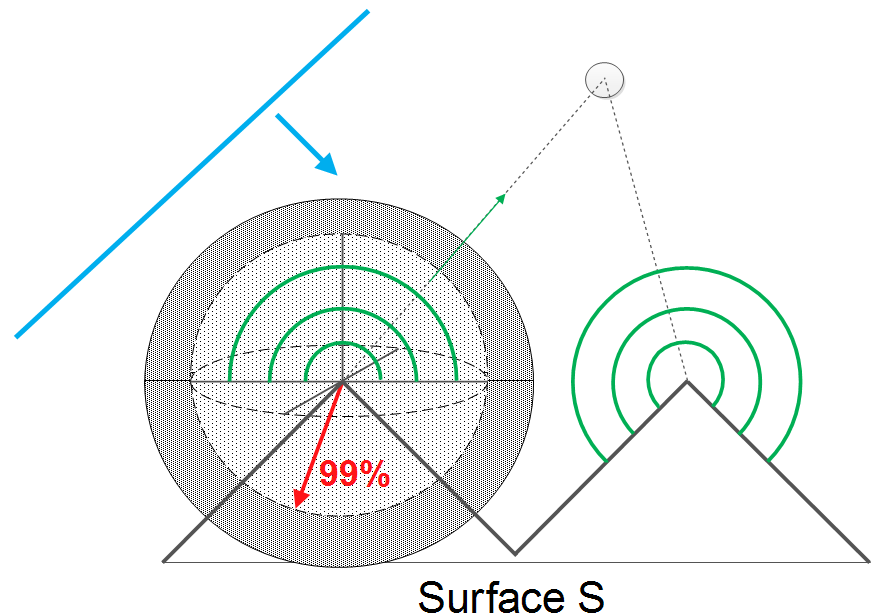
\includegraphics[scale=0.5]{derivation/windowinggaussian.png}
  \caption[Coherence Area using Gaussian Window]{A plane wave encoungers a surface. According to Huygens principle, secondary wavelets are emitted of from this surface. The resulting wave at a certain point in space (here indicated by a gray circle) depends on the inteference among all waves encountering at this position. The amount of significant interference is directly affected by the spatial coherence property of all the wavelets.}
  \label{fig:coherenceareagaussianwindow}  
\end{figure}

Figure $\ref{fig:coherenceareagaussianwindow}$ illustrates the concept of spatial coherence. A wavefront (blue line) encounters a surface. Due to Hugen's Principle, secondary wavelets are emitted off from the surface. The reflected radiance at a certain point in space, e.g. at a viewer's eye position (denoted by the gray circle), is a result of interference among all wavelets at that point. This interference is directly affected by the spatial coherence property of all the emitted wavelets. \\

In physics spatial coherence is predicted by the cross correlation between $t_1$ and $t_2$ and usually modeled by by a Gaussian Random Process. For any such Gaussian Processes we can use a spatial gaussian window $g(x)$ which is equal:

\begin{equation} 
  g(x) = \frac{1}{\sqrt{2\pi}\cdot\sigma}\cdot e^{-\frac{x^2}{2\sigma^2}} 
  \label{eq:gaussianwindowspacial}
\end{equation} 

We have chosen standard deviation $\sigma_s$ of the window such that it fulfills the equation $4 \sigma_s = 65\mu m$. This is equivalent like saying we want to predict about $99.99\%$$\footnote{Standard deviation values from confidence intervals table of normal distribution provided by Wolfram MatheWorld \texttt{http://mathworld.wolfram.com/StandardDeviation.html}.}$ of the resulting spatial coherence interference effects in our model by a cross correlation function. \\

By applying the Fourier Transformation to the spatial window we get the corresponding window in frequency space will look like:
\begin{equation} 
  G(f) = e^{-\frac{f^2}{2\sigma_f^2}}
  \label{eq:gaussianwindowfrequencyspace}
\end{equation} 

Notice that this frequency space window has a standard deviation $\sigma_f$ equal to $\frac{1}{2 \pi \sigma_s}$. Those two windows, the spatial- and the frequency space window, will be used in the next section in order to approximate the DTFT by the DFT by a windowing apporach.

\subsection{Reproduce DTFT by DFT}
\label{sec:gaussianwindow}

In this section we explain how and under what assumptions the DTFT of a discretized signal$\footnote{E.g. a sampled signal like already presented in figure $\ref{fig:ftbydtft}$}$ can be approximated by a DFT. The whole idea how to reproduce the DTFT by DFT is schematically illustrated in figure $\ref{fig:dtftbydft}$.

\begin{figure}[H]
  \centering
  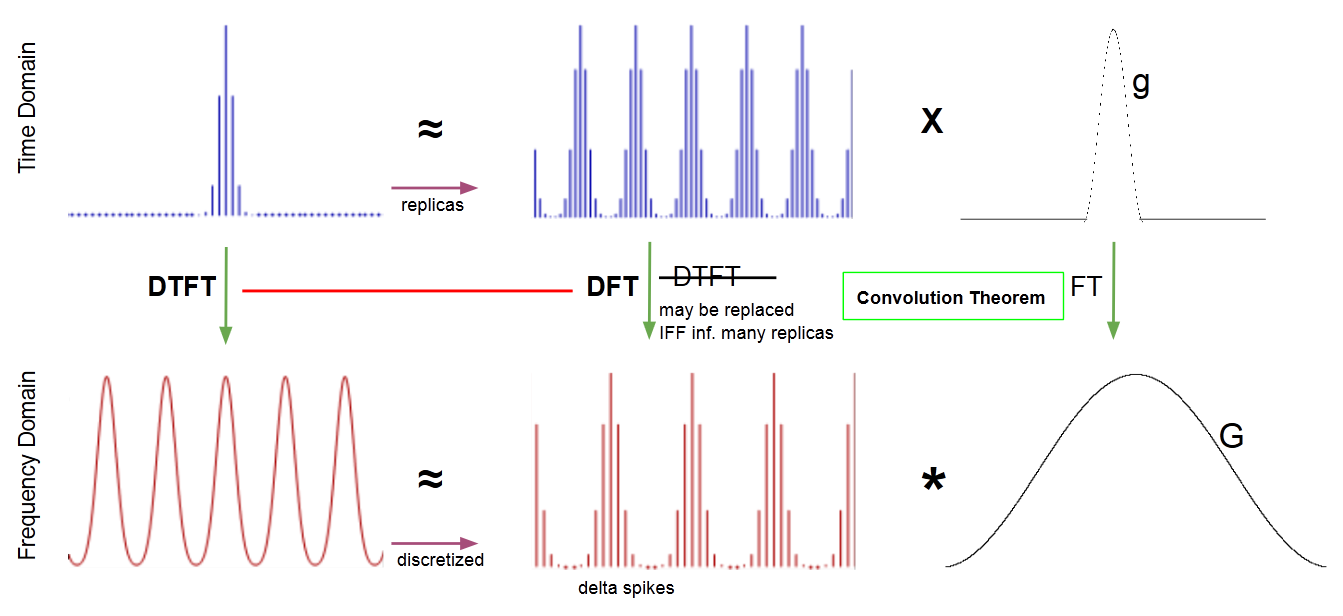
\includegraphics[scale=0.4]{derivation/dtftbydft.png}
  \caption[DTFT by DFT]{Illustration of how to approximate the DTFT $\footnotemark$ by the DFT relying on the Convolution Theorem, using a gaussian window function.}
  \label{fig:dtftbydft}  
\end{figure}
\footnotetext{Images of function plots taken from \texttt{http://en.wikipedia.org/wiki/Discrete\textunderscore Fourier\textunderscore transform} and are modified. Note that the scales in the graphic are not appropriate.} 

Given a spatial, bandlimited and discretized one dimensional signal $\hat{s}$. Our goal is to approximate this spatial signal in a way such that when taking the DTFT of this approximated signal, it will yield almost the same like taking the DTFT of the original sampled $\hat{s}$. For this purpose we will use the previouse introduced concept of gaussian windows and the so called Convolution Theorem which is a fundamental property of all Fourier Transformations. \\

The Convolution Theorem states that the Fourier Transformation of a product of two functions, $f$ and $g$, is equal to convolving the Fourier Transformations of each individual function. Mathematically, this statement corresponds to equation $\ref{eq:convolutiontheorem}$:

\begin{equation} 
  \mathcal{F}\{f\cdot g\} = \mathcal{F}\{f\} * \mathcal{F}\{g\}
  \label{eq:convolutiontheorem}
\end{equation}

The principal issue is how to approximate our given signal $\hat{s}$. Therefore, let us consider another signal $\hat{s_N}$ which is the $N$ times replicated version of $\hat{s}$ (blue signal at center top in figure). \\

Remeber that in general, the signal repsonse at a certain point in space is the result of interference among all signals meeting at that position. In our scenario, the source of those signals are emitted secondary wavelets. The interference strength between these points is related to their spatial coherence. Windowing the signals by a gaussian window $g$ will capture a certain percentage of all interference effects. From the previous section $\ref{sec:spatialcoherenceandwindowing}$ we know that we can use gaussian window like in equation $\ref{eq:gaussianwindowspacial}$ in order to approximate such spatial signals interference effects. \\

Using this insight, we can approximate $\hat{s}$ by taking the product of $\hat{s_N}$ with a gaussian window $g$. This fact is illustrated in the first row of figure $\ref{fig:ftbydtft}$. So what will the DTFT of this approximation yield? We already know that the DTFT of $\hat{s}$ is a continuous, periodic signal, since $\hat{s}$ is bandlimited. Thus, taking the DTFT of this found approximation should give us approximatively the same continuous, periodic signal. \\

This is where the convolution theorem comes into play: Applying the DTFT to the product of $\hat{s_N}$ and $g$ is the same as convolving the DTFT of $\hat{s_N}$ by DTFT of $g$. From equation $\ref{eq:gaussianwindowfrequencyspace}$ we already know that the DTFT of $g$ is just another gaussian, denoted by $G$. On the other hand the DTFT of $\hat{s_N}$ yields a continuous, periodic signal. The higher the value of N, the sharper the signal gets (denoted by delta spiked) and the closer it converges toward to the DFT. This is why the DFT is the limit of a DTFT applied on periodic and discrete signals. Therefore, for a large number of $N$ we can replace the DTFT by the DFT operator when applied on $\hat{s_N}$. \\

Lastly, we see that the DTFT of $\hat{s}$ is approximitely the same like convolving a gaussian window by the DFT of $\hat{s_N}$. This also makes sense, since convolving a discrete, periodic signal (DFT of $\hat{s_N}$) by a continuous window function $G$ yiels a continuous, periodic function. \\

In practise, we cannot compute the DTFT $\ref{eq:dtft}$ numerically due to finite computer arithmetic and hence working with the DFT is our only option. Furthermore, there are numerically fast algorithmes in order to compute the DFT values of a function, the Fast Fourier Transformation (FFT). The DFT $\ref{eq:dft}$ of a discrete height field is equal to the DTFT of an infinitely periodic function consisting of replicas of the same height field. Not, let a spatial gaussian window $g$ having a standard deviation for which $4\sigma_s$ is equal $\mu m$. Then, from before, it followis:

\begin{equation}
\mathcal{F}_{dtft}\{\mathbf{s}\} \equiv \mathcal{F}_{dft} \{\mathbf{s}\} * G(\sigma_f)
\end{equation} 

Therefore we can deduce the following expression from this:

\begin{align}
\mathcal{F}_{dtft} \{\mathbf{t}\}(u,v)
& = \int_{-\infty}^{\infty} \int_{-\infty}^{\infty} {F}_{dft}\{\mathbf{t}\}(w_u,w_v) \phi(u-w_u, v-w_v) dw_u dw_v \nonumber \\
& = \int_{-\infty}^{\infty} \int_{-\infty}^{\infty} \sum_i \sum_j {F}_{dft} \{\mathbf{t}\}(w_u,w_v) \nonumber \\ 
& \quad \quad \delta(w_u-w_i, w_v-w_j)\phi(u-w_u, v-w_v) dw_u dw_v \nonumber \\
& = \sum_i \sum_j \int_{-\infty}^{\infty} \int_{-\infty}^{\infty}  {F}_{dft} \{\mathbf{t}\}(w_u,w_v) \nonumber \\
& \quad \quad \delta(w_u-w_i, w_v-w_j)\phi(u-w_u, v-w_v) dw_u dw_v \nonumber \\
& = \sum_i \sum_j {F}_{dft} \{\mathbf{t}\}(w_u,w_v) \phi(u-w_u, v-w_v)
\end{align}

where 

\begin{equation} \label{eq:gaussweight}
 \phi(x,y) = \pi e^{-\frac{x^2 + y^2}{2\sigma_{f}^2}}
\end{equation} 

\section{Adaption of Stam's BRDF discrete height fields}
\subsection{Rendering Equation}
As already discussed in the theoretical background chapter, colors are associated to radiance. Since we are starting with Stam's BRDF$\footnote{Remember that a BRDF is the portion of a incident light source reflected off a given surface towards a specified viewing direction.}$ formulation but want to perform a simulation rendering structural colors, we have to reformulate this BRDF equation such that we will end up with an identity of the reflected spectral radiance. This is where the rendering equation comes into play. Lets assume we have given an incoming light source with solid angle $\omega_i$ and $\theta_i$ is its angle of incidence, $\omega_r$ is the solid angle for the reflected light. Further let $\lambda$ denote the wavelength$\footnote{Notice that, to keep our terms simple, we have droped all $\lambda$ subscripts for spectral radiance quantites.}$ and $\Omega$ is the hemisphere of integration for the incoming light. Then, we are able to formulate a $BRDF_\lambda$ by using its definition $\ref{eq:defbrdf}$:  

\begin{alignat}{4}
& f_r(\omega_i, \omega_r) &&= \frac{dL_r(\omega_r)}{L_i(\omega_i)cos(\theta_i)d\omega_i} \nonumber \\
\Rightarrow{} & f_r(\omega_i, \omega_r) L_i(\omega_i)cos(\theta_i)d\omega_i &&= dL_r(\omega_r) \nonumber \\
\Rightarrow{} & \int_{\Omega}f_r(\omega_i, \omega_r) L_i(\omega_i)cos(\theta_i)d\omega_i &&= \int_{\Omega}dL_r(\omega_r) \nonumber\\
\Rightarrow{} & \int_{\Omega}f_r(\omega_i, \omega_r) L_i(\omega_i)cos(\theta_i)d\omega_i &&= L_r(\omega_r)
\label{eq:initialbrdf}
\end{alignat}

The last equation is the so called rendering equation $\label{sec:dirlighsourceassumption}$. We assume that our incident light is a directional, unpolarized light source like sunlight and therefore its radiance is given as 

\begin{equation}
 L_{\lambda}(\omega)=I(\lambda)\delta(\omega-\omega_i)
\label{eq:radiancedirlightsource}
\end{equation}

where $I(\lambda)$ is the intensity of the relative spectral power for the wavelength $\lambda$. By plugging the identity in equation $\ref{eq:radiancedirlightsource}$ into our current rendering equation $\ref{eq:initialbrdf}$, we will get:

\begin{align}
L_{\lambda}(w_r) 
& = \int_{\Omega} BRDF_{\lambda}(\omega_i, \omega_r) L_{\lambda}(\omega_i) cos(\theta_i) d\omega_i \nonumber \\
& = BRDF_{\lambda}(\omega_i, \omega_r) I(\lambda) cos(\theta_i)
\label{eq:deribrdfwithdirsource}
\end{align}

where $L_{\lambda}(\omega_i)$ is the incident radiance and $L_{\lambda}(\omega_r)$ is the radiance reflected by the given surface. Note that the integral in equation $\ref{eq:deribrdfwithdirsource}$ vanishes since $\delta(\omega-\omega_i)$ is only equal one if and only if $\omega = \omega_i$.

\subsection{Reflected Radiance of Stam's BRDF}
We are going to use Stam's main derivation $~\eqref{eq:mainstam}$ for the $BRDF(\omega_i, \omega_r)$ in $\ref{eq:deribrdfwithdirsource}$ by applying the fact that the wavenumber is equal $k=\frac{2\pi}{\lambda}$:

\begin{align}
BRDF(\omega_i, \omega_r) 
& = \frac{k^2 F^2 G}{4\pi^2 A w^2} \langle \left|P(ku, kv) \right|^2\rangle \nonumber\\
& = \frac{4 \pi^2 F^2 G}{4\pi^2 A \lambda^2 w^2} \langle \left|P(ku, kv)  \right|^2\rangle \nonumber\\
& = \frac{F^2 G}{A \lambda^2 w^2} \langle \left|P(\frac{2\pi u}{\lambda}, \frac{2\pi v}{\lambda})  \right|^2\rangle
\label{eq:minoradaptedstam}
\end{align}

Going back to equation $\ref{eq:deribrdfwithdirsource}$ and plugging equation $\ref{eq:minoradaptedstam}$ into it, using the definition of equation $\ref{eq:geometricterm}$ and the equation $\ref{eq:sphericalomega}$ for $\omega$ we will get the following:

\begin{align}
L_{\lambda}(\omega_r) 
& = \frac{F^2 (1 + \omega_i \cdot \omega_r)^2}{A \lambda^2 cos(\theta_i)cos(\theta_r)  \omega^2} \left \langle \left|P \left( \frac{2\pi u}{\lambda}, \frac{2\pi v}{\lambda}\right) \right|^2 \right \rangle cos(\theta_i) I(\lambda) \nonumber \\
& = I(\lambda) \frac{F^2 (1 + \omega_i \cdot \omega_r)^2}{\lambda^2 A \omega^2 cos(\theta_r)} \left \langle \left|P \left( \frac{2\pi u}{\lambda}, \frac{2\pi v}{\lambda}\right) \right|^2 \right \rangle
\label{eq:nonrelativebrdffinding}
\end{align}

Note that the Fresnel term $F$ is actually a function of $(w_i, w_r)$, but in order to keep the equations simple, we omitted its arguemts. 
So far we just plugged Stam's BRDF identity into the rendering equation and hence have not significantly deviated from his formulation. Keep in mind that $P$ deontes the Fourier transform of the provided height field which depends on the viewing and incidence light direction. Thus this Fourier Transform has to be recomputed for every direction which will slow down the whole computation quite a lot$\footnote{Even a fast variant of computation the Fourier Transform has a runtime complexitiy of O(N log N) where N is the number of sample.}$. One particular strategy to solve this issue is to approximate $P$ by the Discrete Fourier Transform (DFT)$\footnote{See appendix \ref{chap:appendixsignalprocessing} for further information about different kinds of fourier transformations.}$ and seperate its computation such that terms for many directions can be precomputed and then later retrieved by look ups. The approximation of $P$ happens in two steps: First we approximate the Fourier Transform by the Discrete Time Fourier Transform (DTFT) and then, afterwards, we approximate the DTFT by the DFT. For further about basics of signal processing and Fourier Transformations please consult the appendix $\ref{chap:appendixsignalprocessing}$. \\

Using the insight gained by equation $\ref{eq:sampledsignalfttodtft}$ allows us to further simplify equation $\ref{eq:nonrelativebrdffinding}$:

\begin{align}
L_{\lambda}(\omega_r) 
& = I(\lambda) \frac{F^2 (1 + \omega_i \cdot \omega_r)^2}{\lambda^2 A w^2 cos(\theta_r)} \left \langle \left|P \left( \frac{2\pi u}{\lambda}, \frac{2\pi v}{\lambda}\right) \right|^2 \right \rangle \nonumber \\
& = I(\lambda) \frac{F^2 (1 + \omega_i \cdot \omega_r)^2}{\lambda^2 A w^2 cos(\theta_r)} \left \langle \left|T^2 P_{dtft}\left( \frac{2\pi u}{\lambda}, \frac{2\pi v}{\lambda}\right) \right|^2 \right \rangle
\label{eq:nonrelativebrdffindingreproddtft}
\end{align}

Where $P_{dtft}$ is a substitude for $\mathcal{F}_{DTFT}\{s\}(w)$. Furthermore $T$ the sampling distance for the discretization of $p(x,y)$ assuming equal and uniform sampling in both dimensions $x$ and $y$.

\subsection{Relative Reflectance}
In this section we are going to explain how to scale our BRDF formulation such that all of its possible output values are mapped into the range $\left[0,1\right]$. Such a relative reflectance formulation will ease our life for later rendering purposes since usually color values are within the range $\left[0,1\right]$, too. Furthermore, this will allow us to properly blend the resulting illumination caused by diffraction with a texture map. \\

Let us examine what $L_\lambda(\omega_r)$ will be for a purely specular surface, for which $\omega_r = \omega_0 = \omega_i$ such that $\omega_0 = (0,0,1)$. For this specular reflection case, the correspinding radiance will be denoted as $L_\lambda^{spec}(\omega_0)$. When we know the expression for $L_\lambda^{spec}(\omega_0)$ we would be able to compute the relative reflected radiance for our problem $\ref{eq:nonrelativebrdffinding}$ by simply taking the fraction between $L_\lambda(\omega_r)$ and $L_\lambda^{spec}(\omega_0)$ which is denoted by: 

\begin{equation}
  \rho_\lambda(\omega_i,\omega_r) = \frac{L_\lambda(\omega_r)}{L_\lambda^{spec}(\omega_0)}
  \label{eq:rohrel}
\end{equation}

Notice that the third component $w$ from the vector in equation $\ref{eq:uvw}$ is squared eqaul $(cos(\theta_i)+cos(\theta_r))^2$$\footnote{Consult section $\ref{sec:componentw}$ in the appendix}$. But first, let us derive the following expression:

\begin{align}
L_\lambda^{spec}(\omega_0) 
& = I(\lambda) \frac{F(\omega_0, \omega_0)^2 (1+\colvec[0]{0}{1}\cdot\colvec[0]{0}{1})^2}{\lambda^2 A (cos(0)+cos(0))^2 cos(0)} \langle \left|T_0^2 P_{dtft}(0,0)  \right|^2\rangle \nonumber \\
& = I(\lambda) \frac{F(\omega_0, \omega_0)^2 (1+1)^2}{\lambda^2 A (1+1)^2 1}\left| T_0^2 N_{sample} \right|^2 \nonumber \\
& = I(\lambda) \frac{F(\omega_0, \omega_0)^2}{\lambda^2 A}\left| T_0^2 N_{sample} \right|^2 
\label{eq:lspec}
\end{align}

Where $N_{samples}$ is the number of samples of the DTFT $\ref{eq:dtft}$. Thus, we can plug our last derived expression $\ref{eq:lspec}$ into the definition for the relative reflectance radiance $\ref{eq:rohrel}$ in the direction $w_r$ and will get:

\begin{align}
\rho_\lambda(\omega_i,\omega_r)
& = \frac{L_\lambda(\omega_r)}{L_\lambda^{spec}(\omega_0)} \nonumber \\
& = \frac{I(\lambda) \frac{F(\omega_i, \omega_r)^2 (1 + \omega_i \cdot \omega_r)^2}{\lambda^2 A (cos(\theta_i)+cos(\theta_r))^2 cos(\theta_r)} \langle \left|T_0^2 P_{dtft}(\frac{2\pi u}{\lambda}, \frac{2\pi v}{\lambda}) \right|^2\rangle}{I(\lambda) \frac{F(\omega_0, \omega_0)^2}{\lambda^2 A}\left| T_0^2 N_{sample} \right|^2 } \nonumber \\
& = \frac{F^2(\omega_i,\omega_r)(1 + \omega_i \cdot \omega_r)^2}{F^2(\omega_0,\omega_0)(cos(\theta_i)+cos(\theta_r))^2 cos(\theta_r)} \langle \left|\frac{P_{dtft}(\frac{2\pi u}{\lambda}, \frac{2\pi v}{\lambda})}{N_{samples}}\right|^2\rangle
\label{eq:lspecrohrel}
\end{align}

For simplification and better readability, let us introduce the following expression, the so called gain-factor:

\begin{equation} 
    C(\omega_i,\omega_r) = \frac{F^2(\omega_i,\omega_r)(1 + \omega_i \cdot \omega_r)^2}{F^2(\omega_0,\omega_0)(cos(\theta_i)+cos(\theta_r))^2 cos(\theta_r) N_{samples}^2}
\label{eq:cfact}
\end{equation}

Using equation $\ref{eq:cfact}$, we will get the following expression for the relative reflectance radiance from equation $\ref{eq:lspecrohrel}$:

\begin{equation}
\rho_\lambda(\omega_i,\omega_r) =  C(\omega_i,\omega_r) \langle \left|P_{dtft}(\frac{2\pi u}{\lambda}, \frac{2\pi v}{\lambda})\right|^2\rangle
\label{eq:cpterm}
\end{equation}

Using the previous definition for the relative reflectance radiance equation $\ref{eq:rohrel}$:

\begin{equation}
 \rho_\lambda(\omega_i,\omega_r) = \frac{L_\lambda(\omega_r)}{L_\lambda^{spec}(\omega_0)} 
\end{equation}

Which we can rearrange to the expression: 

\begin{equation}
L_\lambda(\omega_r) = \rho_\lambda(\omega_i,\omega_r)L_\lambda^{spec}(\omega_0)
\label{eq:radianceomegarspec}
\end{equation}

Let us choose $L_\lambda^{spec}(w_0) = S(\lambda)$ such that is has the same profile as the relative spectral power distribution of CIE Standard Illuminant $D65$ discussed in $\ref{subsec:colortransformations}$. Furthermore, when integrating over $\lambda$ for a specular surface, we should get $CIE_{XYZ}$ values corresponding to the white point for $D65$. The corresponding tristimulus values using CIE colormatching functions $\ref{eq:tristimulusvalues}$ for the $CIE_{XYZ}$ values look like:

\begin{align}
X = \int_{\lambda}L_\lambda(\omega_r)\overline{x}(\lambda)d\lambda \nonumber \\
Y = \int_{\lambda}L_\lambda(\omega_r)\overline{y}(\lambda)d\lambda \nonumber \\
Z = \int_{\lambda}L_\lambda(\omega_r)\overline{z}(\lambda)d\lambda
\label{eq:tristimrad}
\end{align}

where $\overline{x}$, $\overline{y}$, $\overline{z}$ are the color matching functions. Combining our last finding from equation $\ref{eq:radianceomegarspec}$ for $L_\lambda(\omega_r)$ with the definition of the tristimulus values from equation $\ref{eq:tristimrad}$, allows us to 
derive a formula for computing the colors values using Stam's BRDF formula relying on the rendering equation $\ref{eq:initialbrdf}$. Without any loss of generality it suffices to derive an explicit expression for just one tristimulus term, for example Y, the luminance:

\begin{align}
Y 
& =\int_{\lambda}L_\lambda(\omega_r)\overline{y}(\lambda)d\lambda \nonumber \\
& =\int_{\lambda}\rho_\lambda(\omega_i,\omega_r)L_\lambda^{spec}(\omega_0) \overline{y}(\lambda)d\lambda \nonumber \\
& =\int_{\lambda}\rho_\lambda(\omega_i,\omega_r) S(\lambda) \overline{y}(\lambda)d\lambda \nonumber \\
& =\int_{\lambda} C(\omega_i,\omega_r) \langle \left|P_{dtft}(\frac{2\pi u}{\lambda}, \frac{2\pi v}{\lambda})\right|^2\rangle S(\lambda) \overline{y}(\lambda)d\lambda \nonumber \\
& = C(\omega_i,\omega_r) \int_{\lambda} \langle \left|P_{dtft}(\frac{2\pi u}{\lambda}, \frac{2\pi v}{\lambda})\right|^2\rangle S(\lambda) \overline{y}(\lambda)d\lambda \nonumber \\
& = C(\omega_i,\omega_r) \int_{\lambda} \langle \left|P_{dtft}(\frac{2\pi u}{\lambda}, \frac{2\pi v}{\lambda})\right|^2\rangle S_y(\lambda)d\lambda
\label{eq:structuralcolorsslow}
\end{align}

Where we used the definition $S_y(\lambda)\overline{y}(\lambda)$ in the last step.

\section{Optimization using Taylor Series}
\label{sec:taylorapproximation}
Our final goal is to render stractural colors resulting by the effect of wave diffraction. So far, we have derived an expression which can be used for rendering. Neverthesless, our current equation $\ref{eq:structuralcolorsslow}$ used for computing structural colors, cannot directly be used for interactive rendering, since $P_{dtft}$ had do be recomputed for every change in any direction$\footnote{According to changes in viewing- or incident light direction.}$. \\

In this section, we will address this issue and deliver an approximation for $P_{dtft}$ defined in equation $\ref{eq:dtftheightfield}$.
This approximation will allow us to seperate $P_{dtft}$ in a certain way such that some computional expsensive terms can be precomputed. The main idea is to formulate $P_{dtft}$ as a series expansion relying on the definition of Taylor Series, like defined in equation $\ref{eq:deftaylor}$. Further, we will provide an error bound for our approximation approach for a given number of terms. Last, we will plug our finding extend our current BRDF formula from equation $\ref{eq:structuralcolorsslow}$ by the findings derived within this section. \\

Let us consider $p(x,y)=e^{ikwh(x,y)}$ form Stam's Paper $\ref{sec:sumstam}$ where $h(x,y)$ is a given height field and $k = \frac{2 \pi}{\lambda}$ denotes the wavenumber of wavelenght $\lambda$. For any complex number $t$ the power series expansion of the exponential function is equal to:
 
\begin{equation}
  e^{t}=1+t+\frac{t^{2}}{2!}+\frac{t^{3}}{3!}+...=\sum_{n=0}^{\infty}\frac{t^{n}}{n!}
  \label{eq:expseriesexpansion}
\end{equation}

Now, when we use the exponent$\footnote{This exponent is a complex valued function, equal to ikwh(x,y).}$ of $p(x,y)$ as an input argument for equation $\ref{eq:expseriesexpansion}$ we get:

\begin{align}
 e^{t}
 &=e^{ikwh} \nonumber \\
 &=1+(ikwh)+\frac{1}{2!}(ikwh)^{2}+\frac{1}{3!}(ikwh)^{3}+... \nonumber \\
 &=\sum_{n=0}^{\infty}\frac{(ikwh)^{n}}{n!}.
 \label{eq:expseriesexpr}
\end{align}

where $i$ is the imaginary unit for complex numbers. For simplification, in the reminder of this section we omitted the arguments of $h$. Equation $\ref{eq:expseriesexpr}$ gives us an expression for an exponential series expansion for an for the exponent of $p(x,y)$. Please note that above's taylor series is convergent for any complex valued number. Therefore the equation $\ref{eq:expseriesexpr}$ is equal to

\begin{equation}
  p(x,y)=\sum_{n=0}^{\infty}\frac{(ikwh(x,y))^{n}}{n!}
  \label{eq:pxyseries}
\end{equation}

and thus gives us a series representation of $p(x,y)$. Next, calculating the Fourier Transformation $\mathcal{F}$ of equation $\ref{eq:pxyseries}$ gives us the identity:

\begin{align}
  \mathcal{F}\left\{ p\right\}
  & \equiv \mathcal{F}\left\{ \sum_{n=0}^{\infty}\frac{(ikwh)^{n}}{n!}.\right\} \nonumber \\
  & \equiv \sum_{n=0}^{\infty}\mathcal{F}\left\{ \frac{(ikwh)^{n}}{n!}\right\} \nonumber \\
  & \equiv \sum_{n=0}^{\infty}\frac{(ikw)^{n}}{n!}\mathcal{F}\left\{ h{}^{n}\right\}
  \label{eq:ftlinopid}
\end{align}

Where we have exploited the fact that the Fourier Transformation is a linear operator. Therefore, in equation $\ref{eq:ftlinopid}$, we have shown that the Fourier Transformation of a series is equal to the sum of the Fourier Transformation, applied on each individual series term. Reusing the identifier $P$$\footnote{This identifier P may be subscripted by \emph{dtft} which will denote the DTFT variant of P.}$ in order to determin the Fourier Transformation of Stams definition $p$ from equation $\ref{eq:px}$, equation $\ref{eq:ftlinopid}$ then correspond to:

\begin{equation}
  P(\alpha,\beta)=\sum_{n=0}^{\infty}\frac{(ikw)^{n}}{n!}\mathcal{F}\left\{ h{}^{n}\right\} (\alpha,\beta)
\end{equation}

Up to now we have found a infinity series representation for $P_{dtft}$. Next we are going to look for an upper bound $N\mathbb{\in N}$ such that 

\begin{align}
  \tilde{P}_{N}(\alpha,\beta)
  :=\sum_{n=0}^{N}\frac{(ikwh)^{n}}{n!}\mathcal{F}\left\{ h{}^{n}\right\} (\alpha,\beta)
  \approx P(\alpha,\beta)
  \label{eq:taylorseriesapproximationofp} 
\end{align}

$\tilde{P}_{N}$ is a good approximation of $P$, i.e. their absolute difference is small$\footnote{Mathematically speaking, this statement correspond to $|| \tilde{P}_{N} - P|| \leq \epsilon$, where $\epsilon$ > 0 is a small number.}$. But first, the following two facts would have to be proven$\footnote{Please have a look in section $\ref{chap:taylorseriesapproxappendix}$ in the appendix}$:

\begin{enumerate}
\item Show that there exist such an $N\mathbb{\in N}$ s.t. the approximation of equation $\ref{eq:taylorseriesapproximationofp}$ holds true.
\item Find a value for $N$ s.t. this approximation is below a certain error bound, e.g. close to machine precision $\epsilon$. 
\end{enumerate}

Assuming these facts are proven and there actually exists such an $N$, we can make use of the taylor series approximation from equation $\ref{eq:taylorseriesapproximationofp}$ and use it for approximating $P_{dtft}$. This idea allows us to adapt equation $\ref{eq:structuralcolorsslow}$, which is used for computing the structural colors of our BRDF model, in nummerically fast way. E.g. the equation for the luminance is then be equal:

\begin{align}
Y 
& = C(w_i,w_r) \int_{\lambda} \langle \left|P_{dtft}(\frac{2\pi u}{\lambda}, \frac{2\pi v}{\lambda})\right|^2\rangle S_y(\lambda)d\lambda \nonumber \\
& = C(w_i,w_r) \int_{\lambda} \left| \sum_{n=0}^N \frac{(wk)^n}{n!} \mathcal{F}\{i^n h^n\}(\frac{2\pi u}{\lambda}, \frac{2\pi v}{\lambda})\right|^2 S_y(\lambda)d\lambda
\label{eq:xcolexpression}
\end{align}

Notice that equation $\ref{eq:xcolexpression}$ is contrainted by $N$ and hence is an approximation of equation $\ref{eq:structuralcolorsslow}$. Furthermore, it is possible to seperate out all the Fourier Terms in the summation and precompute them. This is why the approach in equation $\ref{eq:xcolexpression}$ is fast in order to compute structural color values according to our BRDF model.

\section{Spectral Rendering}
\label{sec:spectralrendering}
As the last step of our series of derivations, we plug all our findings together to one big equation. in order to compute the color for each pixel on our mesh in the $CIE_{XYZ}$ colorspace. For any given heigh-field $h(x,y)$ representing a grating of a nano structure and for given direction vectors $w_i$ and $w_r$ as shown in figure $\ref{fig:geometricsetup}$ the resulting color caused by the effect of diffraction can be computed the following way:

\begin{equation}
DFT_{n}\{h\}(u,v) = {F}_{dft}\{i^n h^n\}(\frac{2\pi u}{\lambda},\frac{2\pi v}{\lambda})
\end{equation}

\begin{equation}
  W_{n}(u,v) = \sum_{(r,s) \in \mathcal{N}_1(u,v)} \left| DFT_{n}\{h\}(u-w_r, v-w_s) \right|^2 \phi(u-w_r, v-w_s)
\end{equation}
where $\phi(x,y) = \pi e^{-\frac{x^2 + y^2}{2\sigma_{f}^2}}$ is the Gaussian window from equation $\ref{sec:gaussianwindow}$ and $\mathcal{N}_1(u,v)$ denotes the one-neighborhood around $(u,v)$. Then $\forall (u,v,w)$ liked defined in equation $\ref{eq:uvw}$, our final expression for computing structural colors due to diffraction, using our previous derivations, will be equal:

\begin{equation}
\begin{split}
\colvec[X]{Y}{Z}& = C(\omega_i,\omega_r) \int \limits_{\lambda} \sum_{n=0}^N  \frac{(2 \pi w)^n}{\lambda^n n!} W_{n}(u,v) \colvec[S_x(\lambda)]{S_y(\lambda)}{S_z(\lambda)}d\lambda
\end{split}
\label{eq:finalexpression}
\end{equation}

\section{Alternative Approach}
\subsection{PQ factors}
\label{sec:pq}
In this section we are presenting an alternative approach to the previous Gaussian window approach 
$\ref{sec:gaussianwindow}$ 
in order to solve the issue working with $DTFT$ instead the $DFT$. We assume, that a given surface $S$ is covered by a number of replicas of a provided representative surface patch $f$. In a simplified, one dimensional scenario, mathematically speaking, $f$ is assumed to be a repetative function, i.e. $\forall x \in \mathds{R} : S(x) = S(x+nT)$, where $T$ is its period and $n \in \mathds{N}_{0}$. Thus, the surfaces can be written formally as:

\begin{equation}
  S(x) = \sum_{n=0}^N f(x+nT)
\label{eq:replicatedpatchsurface}
\end{equation}

What we are looking for is an identity for the Fourier Transform$\footnote{Remember that we are using the definiton of Fourier Transform used in electrical engineering where $\mathcal{F}$ actually corresponds to the inverse Fourier Transform.}$ of our surface $S$, required in order to simplify the $(X,Y,Z)$ colors from $\ref{eq:xcolexpression}$:

\begin{align}
\mathcal{F}\{S\}(w)
& =\int f(x) e^{iwx}dx \nonumber \\
& =\int_{-\infty}^{\infty} \sum_{n=0}^{N} f(x+nT) e^{iwx}dx \nonumber \\
& =\sum_{n=0}^{N} \int_{-\infty}^{\infty} f(x+nT) e^{iwx}dx
\label{eq:pqsinit}
\end{align}

Next, apply the following substitution $x+nT = y$ which will lead us to:

\begin{gather}
x=y-nT \nonumber \\
dx=dy
\label{eq:substitude1dpq}
\end{gather} 

Plugging this substitution back into equation $\ref{eq:pqsinit}$ we will get: 

\begin{align}
\mathcal{F}\{S\}(w)
& =\sum_{n=0}^{N} \int_{-\infty}^{\infty} f(x+nT) e^{iwx}dx \nonumber \\
& =\sum_{n=0}^{N} \int_{-\infty}^{\infty} f(y) e^{iw(y-nT)}dy \nonumber \\
& =\sum_{n=0}^{N} e^{-iwnT} \int_{-\infty}^{\infty} f(y) e^{iwy}dy \nonumber \\
& =\sum_{n=0}^{N} e^{-iwnT} \mathcal{F}\{f\}(w) \nonumber \\
& =\mathcal{F}\{f\}(w) \sum_{n=0}^{N} e^{-iwnT}
\label{eq:pqsub}  
\end{align}

We used the fact that the exponential term $e^{-iwnT}$ is a constant factor when integrating along $dy$ and the identity for the Fourier Transform of the function $f$. Next, let us examine the series $\sum_{n=0}^N e^{-iwnT}$ closer:

\begin{align}
\sum_{n=0}^N e^{-uwnT}
& =\sum_{n=0}^N (e^{-iwT})^n \nonumber \\
& =\frac{1-e^{iwT(N+1)}}{1-e^{-iwT}}
\label{eq:pqgeometricseries}
\end{align}

We recognize the geometric series identity for the left-hand-side of equation $\ref{eq:pqgeometricseries}$. Mainly relying on trigonometric identities, equation $\ref{eq:pqsub}$ can further simplified to:  

\begin{align}
\mathcal{F}\{S\}(w)
& = (p+iq) \mathcal{F}\{f\}(w)  
\label{eq:mainfinding1d}
\end{align}

where $p$ and $q$ are defined like:

\begin{align}
p& =\frac{1}{2}+\frac{1}{2}\left(\frac{cos(wTN)-cos(wT(N+1))}{1-cos(wT)}\right) \nonumber \\
q& =\frac{sin(wT(N+1))-sin(wTN)-sin(wT)}{2(1-cos(wT))}
\end{align}

Please notice, all derivation steps can be found in the appendix in section $\ref{sec:pqonedimappendix}$. \\

Now lets consider our actual problem description. Given a patch of a nanoscaled sureface snake shed represented as a two dimensional heightfield $h(x,y)$. We once again assume that this provided patch is representing the whole surface $S$ of our geometry by some number of replicas of itself. Therefore, $S(x,y) = \sum_{n=0}^{N} h(x+nT_1, y+mT_2)$, assuming the given height field has the dimensions $T_1$ by $T_2$. In order to derive an identity for the two dimensional Fourier transformation of $S$ we can similarly proceed like we did to derive equation $\ref{eq:mainfinding1d}$.

\begin{align}
\mathcal{F}\{S\}(w_1, w_2)
& =(p + iq) \mathcal{F}_{DTFT}\{h\}(w_1,w_2)
\label{eq:pqmainfinding}
\end{align}

Where all derivation steps can be found in the appendix in section $\ref{sec:pqtwodimappendix}$ and we have defined 

\begin{align}
p := (p_1 p_2 - q_1 q_2) \nonumber \\ 
q := (p_1 p_2 + q_1 q_2)
\label{eq:pqsubst2}
\end{align}

For the identity of equation $\ref{eq:pqmainfinding}$ we made use of Green's integration rule which allowed us to split the double integral to the product of two single integrations. Also, we used the definition of the 2-dimensional inverse Fourier transform of the height field function. We applied a similar substitution like we did in $\ref{eq:substitude1dpq}$, but this time twice, once for $x_1$ and once for $x_2$ separately. The last step in equation $\ref{eq:pqmainfinding}$, substituting with $p$ and $q$ in equation $\ref{eq:pqsubst2dappendix}$ will be useful later in the implementation. The insight should be, that the product of two complex numbers is again a complex number. We will have to compute the absolute value of $\mathcal{F}\{S\}(w_1,w_2)$ which will then be equal $(p^2 + q^2)^{\frac{1}{2}}\left|\mathcal{F}\{h\}(w_1,w_2)\right|$


\subsection{Interpolation}
\label{sec:sincinterpolation}

In $\ref{sec:pq}$ we have derived an alternative approach when we are working with a periodic signal instead using the gaussian window approach from $\ref{sec:gaussianwindow}$. Its main finding $\ref{eq:pqmainfinding}$ that we can just integrate over one of its period instead iterating over the whole domain. Nevertheless, this main finding is using the inverse DTFT. Since we are using 

We are interested in recovering an original analog signal $x(t)$ from its samples $x[t] = $ 

Therfore, for a given sequence of real numbers $x[n]$, representing a digital signal, its correspond continuous function is: 

\begin{equation}
  x(t) = \sum_{n=-\infty}^{\infty} x[n] sinc\left(\frac{t-nT}{T}\right)
\end{equation}

which has the Fourier transformation $X(f)$ whose non-zero values are confined to the region $|f| \leq \frac{1}{2T} = B$.
When $x[n]$ represents time samples at interval $T$ of a continuous function, then the quantity $f_s = \frac{1}{T}$ is known as its sample rate and $\frac{f_s}{2}$ denotes the Nyquist frequency. The sampling Theorem states that when a function has a Bandlimit B less than the Nyquist frequency, then $x(t)$ is a perfect reconstruction of the original function. 

\begin{figure}[ht]
  \centering
  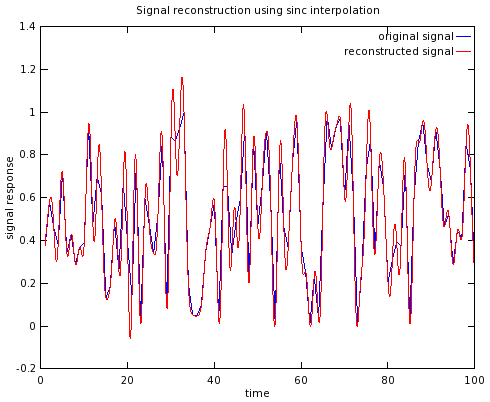
\includegraphics[scale=0.8]{background/sincreconstructed.png}
  \caption{Comparission between a given random one dimensional input signal $s(t)$ and its sinc interpolation $\hat{s}(t)$. Notice that for the interpolation there were $N=100$ samples from the original signal provided.}
  \label{fig:plotsincinterpolation}  
\end{figure}

\newpage{\pagestyle{empty} \cleardoublepage}
% % 
% \chapter{Implementation}
In computer graphics, we generally synthesize 2d images from a given 3d scene description$\footnote{A usual computer graphics scene consist of a viewer's eye, modeled by a virtuel camera, light sources and geometries placed in the world, having some material properties assigned to.}$. This process is denoted as rendering. A usual computer graphics scene consist of a viewer's eye, modeled by a virtuel camera, light sources and geometries placed in the world$\footnote{With the term world we are refering to a global coordinate system which is used in order to place all objects.}$, having some material properties$\footnote{Example material properties are: textures, surface colors, reflectance coefficients, refractive indices and so on.}$ assigned to. In our implementation, scene geometries are modeled by triangular meshes for which each triangle is represented by a triple of vertices. Each vertex has a position, a surface normal and a tangent vector associated with. \\

The process of rendering basically involves a mapping of 3d sceene objects to a 2d image plane and the computation of each image pixel's color according to the provided lighting, viewing and material information of the given scene. These pixel colors are computed in several statges in so called shader programs, directly running on the Graphic Processing Unit (GPU) hardware device. In order to interact with a GPU, for our implementations, we rely on the programing interface of OpenGL$\footnote{Official website:\texttt{http://www.opengl.org/}}$, a cross-language, multiplattform API. In OpenGL, there are two fundamental shading pipeline stages, the vertex- and the fragment shading stage, each applied sequentially. Vertex shaders apply all transformations to the mesh vertices and pass this data to the fragment shaders. Fragment shaders receive linearly interpolated vertex data of a particular triangle. They are responsible to compute the color of his triangle. \\

In this chapter we explain in detail a technique for rendering structural colors due to diffraction effects on natural graings, based on the model we have derived in the previouse chapter $\ref{chap:derivations}$, summarized in section $\ref{sec:spectralrendering}$. For this purpose we implemented a reference framework which is based on a class project of the lecture \emph{Computer Graphics} held by Mr. M. Zwicker which I attended in autum 2012$\footnote{The code of underlying reference framework is written in Java and uses JOGL and GLSL$\footnotemark$ in order to comunicate with the GPU and can be found at \texttt{https://ilias.unibe.ch/}}$. \\
$\footnotetext{JOGL is a Java binding for OpenGL (official website \texttt{http://jogamp.org/jogl/www/}) and GLSL is OpenGL's high-level shading language. Further information can be found on wikipedia: \texttt{http://de.wikipedia.org/wiki/OpenGL\textunderscore Shading\textunderscore Language}}$

For performing the rendering process, our implementation expects being provided by the following input data$\footnote{All data is provided by the Laboratory of Artificial and Natural Evolition in Geneva. See their website:\texttt{www.lanevol.org}}$:
\begin{itemize}
  \item the structure of snake skin of different species$\footnote{We are using height field data for Elaphe and Xenopeltis snakes individuals like shown in figure $\ref{fig:snakespecies}$}$ represented as discrete valued height fields acquired using AFM and stored as grayscale images.
  \item real measured snake geometry represented as a triangle mesh.
\end{itemize}

The first processing stage of our implementation is to compute the Fourier Terms of the provided height fields like described in section $\ref{sec:taylorapproximation}$. For this preprocessing purpose we use Matlab relying on its internal, numerically fast, libraries for computing Fourier Transformations$\footnote{Actually we use Matlab's inverse 2d Fast Fourier Transformation (FFT) implementation applied on different powers of quation $\ref{eq:px}$. Further information can be read up in section $\ref{sec:precompmatlabfourierimages}$}$. The next stage is to read these precomputed Fourier Terms into our Java renderer. This program also builds our manually defined rendering scene. The last processing stage of our implementation is rendering of the iridescent colorpatterns due to light diffracted on snake skins. We implemented our diffraction model from chapter $\ref{chap:derivations}$ as OpenGL shaders. Notice that all the necessary computations in order to simulate the effect of diffraction are performed within a fragment shader. This implies that we are modeling pixelwise the effect of diffraction and hence the overall rendering quality and runtime complexity depends on rendering window's resolution. \\

In the following sections of this chapter we are going to explain all render processing stages in detail. First, we discuss, how our precomputation process, using Matlab, actually works. Then, we introduce our Java Framework. It is followed by the main section of this chapter, the explanation how our OpenGL shaders are implemented. The last section discusses an optimization of our fragment shader such that it will have interactive runtime.

\section{Precomputations in Matlab}
\label{sec:precompmatlabfourierimages}
Our first task is to precompute the two dimensional discrete Fourier Fransformations$\ref{eq:dftnterm}$ for a given height field, representing a natural grating. For that purpose we have written a small Matlab $\footnote{Matlab is a interpreted scripting language which offers a huge collection of mathematical and numerically fast and stable algorithms.}$ script conceptialized in algorithm $\ref{alg:matlabprecomp}$. Our Matlab script reads a given image, which is representing a nano-scaled height field, and computes its two dimensional DFT (2dDFT) by using Matlab's internal Fast Fourier Transformation (FFT) function, denoted by $ifft2$$\footnote{Remember, even we are talking about fourier transformations, in our actual computation, we have to compute the inverse fourier transformation. See paragraph $\ref{sec:electricalengeneeringftconvention}$ for further information. Furthermore our height fields are two dimensional and thus we have to compute a 2d inverse fourier transformation.}$. Note that we only require one color channel of the input image, since the input image is representing an height field, encoded by just one color. Keep in mind that taking the Fourier transformation of an arbitrary function will result in a complex valued output which implies that we will get a complex value for frequency pairs of our input image. Therefore, for each input image we get as many output images, representing the 2dDFT, as the minimal number of taylor terms required for a well-enough approximation. In order to store our output images, we have to use two color channels instead of just one like it was for the given input image. Some example visualizations for the Fourier Tranformation are shown in figure $\ref{fig:matlabBlazeFourierImages}$. We store these intermediate results as binary files to offer floating point precision for the run-time computations to ensure higher precision. \\

In our script every discrete frequency is normalized by its corresponding DFT extrema$\footnote{We are talking about the i2dFFT of our height fields to the power of n. This is an N by N matrix (assuming the discrete height field was an N by N image), for which each component is a complex number. Hence, there is a a complex extrema as well as a imaginary extrema.}$ in the range $\left[0,1\right]$ and the range extrema are stored seperately for each DFT term. The normalization is computed the following way: 

\begin{align}
  f:\left[x_{min},x_{max}\right]\to \left[0,1\right] \nonumber\\
  x \mapsto f(x) = \frac{x-x_{min}}{x_{max}-x_{min}}
\label{eq:dfttermnormalization}
\end{align}
Where $x_{min}$ and $x_{max}$ denote the extreme values of a DFT term. Later, during the shading process of our implementation, we have to apply the inverse mapping. This is non-linear interpolation which is required in order to rescaled all frequency values in the DFT terms. 

\begin{algorithm}[H]
\caption{Precomputation: Pseudo code to generate Fourier terms}
\textbf{INPUT} \ $heightfieldImg, \ maxH, \ dH, \ termCnt$ \\
\textbf{OUTPUT} \ $DFT \ terms \ stored \ in \ Files$
\begin{lstlisting}
% maxH:    A floating-point number specifying 
%          the value of maximum height of the 
%          height-field in MICRONS, where the 
%          minimum-height is zero. 
%         
% dH:      A floating-point number specifying 
%          the resolution (pixel-size) of the 
%          'discrete' height-field in MICRONS. 
%          It must be less than 0.1 MICRONS 
%          to ensure proper response for 
%          visible-range of light spectrum.
%
% termCnt: An integer specifying the number of 
%          Taylor series terms to use.

function ComputeFFTImages(heightfieldImg, maxH, dh, termCnt)
dH = dh*1E-6;
% load patch into heightfieldImg
patchImg = heightfieldImg.*maxH;
% rotate patchImg by 90 degrees
for t = 0 : termCnt
  patchFFT = power(1j*patchImg, t);
  fftTerm{t+1} = fftshift(ifft2(patchFFT));
  
  % rescale terms as
  imOut(:,:,1)  = real(fftTerm{t+1});
  imOut(:,:,2)  = imag(fftTerm{t+1});
  imOut(:,:,3)  = 0.5;
  
  % rotate imOut by -90 degrees
  % find real and imaginary extrema of 
  % write imOut, extrema, dH, into files.
end
\end{lstlisting}
\label{alg:matlabprecomp}
\end{algorithm}

They key idea of algorithm $\ref{alg:matlabprecomp}$ is to compute iteratively the Fourier Transformation for different powers of the provided height field. These DFT values are scaled by according to their extrema values. Another note about the command fftshift: It rearranges the output of the ifft2 by moving the zero frequency component to the centre of the image. This simplifies the computation of DFT terms lookup coordinates during rendering.

\label{sec:precompmatlabfft}
\begin{figure}[H]
  \centering
  \subfigure[Heightfield of a Blazed Grating]{
    
\includegraphics[scale=0.25]{implementation/hf/blaze/blazeBig.png}
    \label{fig:matlabBlazePatch}
  }
~
  \subfigure[Plot of extreme values for different powers of blazed grating]{
    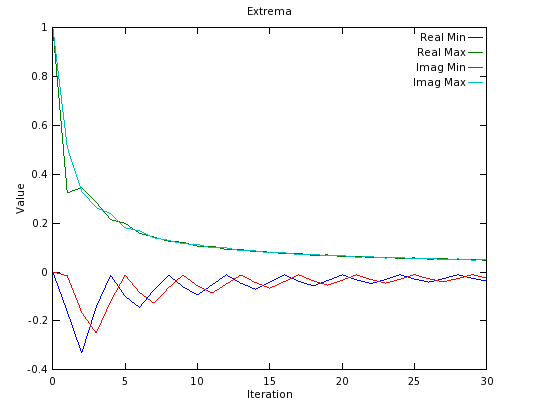
\includegraphics[scale=0.4]{implementation/hf/blaze/extrema.png}
    \label{fig:extremaBlaze}  
  }
  
  \subfigure[ImRe0]{
    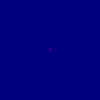
\includegraphics[scale=0.6]{implementation/hf/blaze/AmpReIm0.png}
    \label{fig:blazeftimre0}
  }
~
  \subfigure[ImRe1]{
    
\includegraphics[scale=0.6]{implementation/hf/blaze/AmpReIm1.png}
    \label{fig:blazeftimre1}
  }
~
  \subfigure[ImRe4]{
    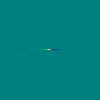
\includegraphics[scale=0.6]{implementation/hf/blaze/AmpReIm4.png}
    \label{fig:blazeftimre4}
  }
~
  \subfigure[ImRe10]{
    
\includegraphics[scale=0.6]{implementation/hf/blaze/AmpReIm10.png}
    \label{fig:blazeftimre10}
  }
~
  \subfigure[ImRe20]{
    
\includegraphics[scale=0.6]{implementation/hf/blaze/AmpReIm20.png}
    \label{fig:blazeftimre20}
  }
 
  
  \subfigure[Re0]{
    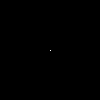
\includegraphics[scale=0.6]{implementation/hf/blaze/re0.png}
    \label{fig:blazeftre0}
  }
~
  \subfigure[Re1]{
    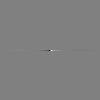
\includegraphics[scale=0.6]{implementation/hf/blaze/re1.png}
    \label{fig:blazeftre1}
  }
~
  \subfigure[Re4]{
    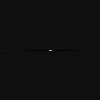
\includegraphics[scale=0.6]{implementation/hf/blaze/re4.png}
    \label{fig:blazeftre4}
  }
~
  \subfigure[Re10]{
    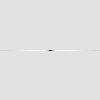
\includegraphics[scale=0.6]{implementation/hf/blaze/re10.png}
    \label{fig:blazeftre10}
  }
~
  \subfigure[Re20]{
    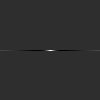
\includegraphics[scale=0.6]{implementation/hf/blaze/re20.png}
    \label{fig:blazeftre20}
  }
  
  \subfigure[Im0]{
    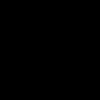
\includegraphics[scale=0.45]{implementation/hf/blaze/im0.png}
    \label{fig:blazeftim0}
  }
~
  \subfigure[Im1]{
    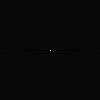
\includegraphics[scale=0.6]{implementation/hf/blaze/im1.png}
    \label{fig:blazeftim1}
  }
~
  \subfigure[Im4]{
    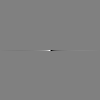
\includegraphics[scale=0.6]{implementation/hf/blaze/im4.png}
    \label{fig:blazeftim4}
  }
~
  \subfigure[Im10]{
    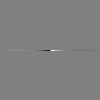
\includegraphics[scale=0.6]{implementation/hf/blaze/im10.png}
    \label{fig:blazeftim10}
  }
~
  \subfigure[Im20]{
    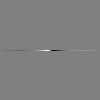
\includegraphics[scale=0.6]{implementation/hf/blaze/im20.png}
    \label{fig:blazeftim20}
  }
  
  \caption[DFT Terms for a Blazed grating]{A visualization of DFT terms for a height field of a Blazed Grating.}
  \label{fig:matlabBlazeFourierImages}
\end{figure}

In figure $\ref{fig:matlabBlazeFourierImages}$ we see examples of a visualization of Fourier Transformations generated by our Matlab script for a blazed grating$\footnote{A blazed grating is a height field consisting of ramps, periodically aligned on a given surface.}$ as an input height field image, shown in figure $\ref{fig:matlabBlazePatch}$. Figure $\ref{fig:extremaBlaze}$ shows plots of the extreme values of DFT terms for different powers of the blazed grating. We recognize that, the higher the power of the grating becomes, the closer the extreme values of the corresponding DFT terms get. The figure line from figure $\ref{fig:blazeftimre0}$ until figure $\ref{fig:blazeftimre20}$ show us example visualizations of DFT terms for different powers of our grating's height field. Remember that DFT terms are complex valued matrices of dimension as their height field has. In this visualization, all real part values are stored in the red- and the imaginary parts in the green color channel of an DFT image. The figure line from figure $\ref{fig:blazeftre0}$ till figure $\ref{fig:blazeftre20}$ show us the real part images from above's line corresponding figures. Similarly for the figur line from figure $\ref{fig:blazeftim0}$ until figure $\ref{fig:blazeftim20}$ showing the correspinding imaginary part DFT term images.

\section{Java Renderer}
This section explains the architecture of the rendering program which I implemented$\footnote{This program is based on the code of a java real-time renderer, developed as a student project in the computer graphics class, held by M. Zwicker in autumn 2012.}$ and used for this project. The architecture of the program is divided into two parts: a rendering engine, the so called jrtr (java real time renderer) and an application program. Figure $\ref{fig:rendererArchitecture}$ outlines the architecture of the renderer. 

\begin{figure}[H]
  \centering
  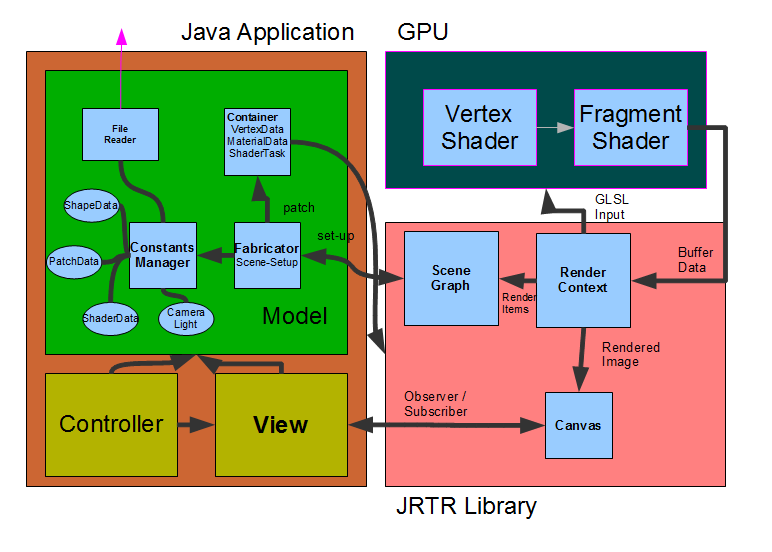
\includegraphics[scale=0.7]{implementation/framework.png}
  \caption[Renderer Architecture]{Schematical architecture of our Java renderer.}
  \label{fig:rendererArchitecture}
\end{figure}

The application program relies on the MVC (Model-View-Controller) architecture pattern. The View just represents a canvas in which the rendered images are shown. The Controller implements the event listening functionalities for interactive rendering within the canvas. The Model of our application program consists of a Fabricator, a file reader and a constants manager. The main purpose of a Fabricator is to set up a rendering scene by accessing a constant manager containing many predefined scene constants. A scene consists of a camera, a light source, a frustum, shapes and their associated material constants. Such materials include a shape texture, precomputed DFT terms$\footnote{See section \ref{sec:precompmatlabfourierimages} for further information.}$ for a given height field$\footnote{and other height field constants such as the maximal height of its bumps or its pixel real-world width correspondance.}$ like visualized in figure $\ref{fig:matlabBlazeFourierImages}$. A shapes is a geometrical object defined by a triangular mesh as shown in figure $\ref{fig:wireframemesh}$. 

\begin{figure}[H]
  \centering
  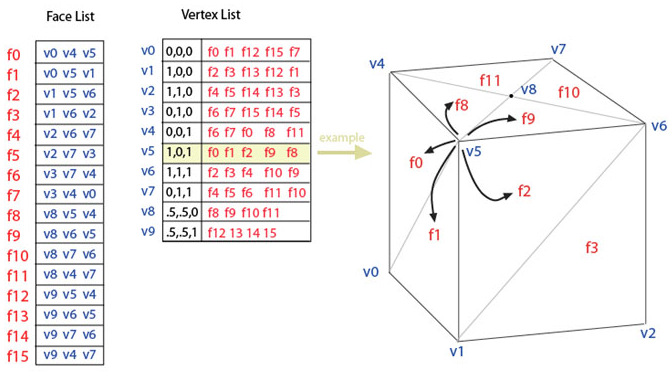
\includegraphics[scale=0.7]{implementation/wireframemesh.png}
  \caption[Triangular Mesh]{Representation$\footnotemark$ of a triangular mesh represents an object as a set of triangles and a set of vertices.}
  \label{fig:wireframemesh}
\end{figure}
\footnotetext{Modified image which originally has been taken from \texttt{http://en.wikipedia.org/wiki/Polygon\textunderscore mesh}}

Such a mesh is represented as a data structure consisting of a list of vertices, each stored as a triplet of $x$, $y$, $z$ positions and triangles, each defined by a triple of vertex-indices. Besides its position, a vertex can have further data assigned to, like a surface color, normals and texture coordinates. The whole scene is encapsulated in a scene graph data-structures, defined and managed within the rendering engine. A scene graph contains all scene geometries and their transformations in a tree like structured hierarchy. \\

All required configuration, in oder to communicate with the GPU through OpenGL, is performed in the jrtr rendering engine. Furthermore, jrtr's render context object, the wholeresource-management for various types of low-level buffers, which are used within the rendering pipeline by our GLSL shaders, takes place in the rendering place. More precisely, this means allocating memory for the buffers, assigning them with scene data and flushing them, when not used anymore. The whole shading process is performed in the GPU, stage-wise: The first stage is the vertex shader (see section $\ref{sec:vertexshader}$) followed by the fragment shader (see section $\ref{sec:fragmentshader}$). The jrtr framework also offers the possibility to assign user-defined shaders written in GLSL.

\section{GLSL Diffraction Shader}
\subsection{Vertex Shader}
\label{sec:vertexshader}

%purpose


%%%%%%%%%%%%%%%%%%%%%%%%%%%%%%%%%%%%%%%%%%%
In our implementation we want to simulate the structural colors a viewer sees when light diffracted is on grating, e.g. on the skin of a snake. For this purpose, we reproduce a 2d image of a given 3d scene as seen from the perspective of a viewer for given lightning conditions. The color computation of an image is performed in the GPU shaders of the rendering pipeline. In OpenGL, there are two basic shading stages performed to rendern an image whereas the vertex shader is the first shading stage in the rendering pipeline. \\

As an input, a vertex shader receives one vertex of a mesh and other vertex data such as a vertex normals. It only can access this data and has no information about the neighborhood of a vertex or the topology of its corresponding shape. Since vertex positions of a shape are defined in a local coordinate system$\footnote{Defining the positions of a shape in a local coordinate system simplifies its modeling process and allows us to apply transformations to a shape.}$ and we want to render an image of the perspective of viewer, we have to transform the locally defined positions to a perspectively projected viewer space. Therefore, the main purpose$\footnote{Furthermore, texture coordinates used for texture-lookup within the fragment shader and per vertex lightning can be computed.}$ of a vertex shader is to tranform the position of vertices. Notice that a vertex shader can manipulate the position of a vertices, but cannot generate additional mesh vertices. Therfore, the output of any vertex shader is a transformed vertex position. Keep in mind that all vertex shader outputs will be used within the fragment shader. For an example, please have a look at our fragment shader $\ref{sec:fragmentshader}$. \\

In the following let us consider the whole transformation, applied in the vertex shader, in depth. Let $p_{local}$ denote the position of a shape vertex, defined in a local coordinate system. Then the transformation from $p_{local}$
into the perspective projected position as seen by a observer $p_{projective}$ looks like the following:
\begin{equation}
  p_{projective} = P \cdot C^{-1} \cdot M \cdot p_{local}
  \label{eq:vertextransformation}
\end{equation}

where $P$, $C^{-1}$ and $M$ are transformation matrices$\footnote{These tranformation matrices are linear transformations expressed in homogenous coordinates.}$, defined the following way:
\begin{description}
\item[Model matrix $M$:] Each vertex position of a shape is initially defined in a local coordinate system. To make is feasible to place and transform shapes in a scene, a reference coordinate system, the so called world space, has to be introduced. Hence, for every shape a matrix $M$ is associated, defining the transformation from its local coordinate system into the world space. 
\item[Camera matrix $C$:] A camera models how the eye of a viewer sees an object, defined in world space like shown in figure $\ref{fig:cameracoordinatesystem}$. For calculating the transformation matrix $C$, a viewer's eye position and viewing direction, each defined in world space, are required. Therefore, $C$ denotes a transformation from coordinates defined in camera space into the world space. Thus, in order to transform a position from world space to camera space, we have to use the inverse of $C$, denoted by $C^{-1}$. 
\item[Frustum $P$:] The Matrix P defines a perspective projection onto image plance, i.e. for any given position in camera space, $P$ determines the corresponding 2d image coordinate. Persepctive projections project along rays that converge in center of projection.
\end{description}

Since we are interested in modeling how a viewer sees structural colors on a given scene shape as shown in figure $\ref{fig:cameracoordinatesystem}$, modeling a viewer's eye by formulating the corresponding camera matrix $C$, is the most important component of the whole transformation series applied in the vertex shader. Hence, we next will have a closer look in how a camera matrix $C$ actually can be computed. 

\begin{figure}[H]
  \centering
  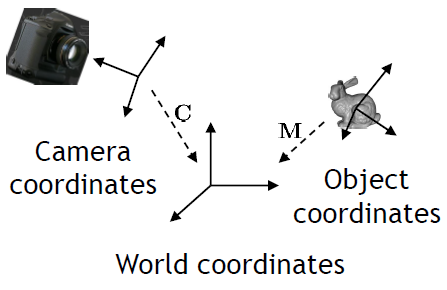
\includegraphics[scale=0.7]{implementation/cameracoodsyst.png}
  \caption[Camera Coordinate System]{Illustration$\footnotemark$ of the Camera coordinate system where its origin defines the center of projection of camera.}
  \label{fig:cameracoordinatesystem}
\end{figure}
\footnotetext{This image has been taken from the lecture slides of computer graphics class 2012 which can be found on ilias.}

The camera matrix $C$ is constructed from its center of projection $e$, the position $d$ where the cameras looks at and a direction vector $up$, defining what is the direction in camera space pointing upwards. These components, $e$, $d$ and $up$, are defined in world coordinates. Figure $\ref{fig:cameramatrix}$ illustrates geometrical setup required in order to construct $C$.

\begin{figure}[H]
  \centering
  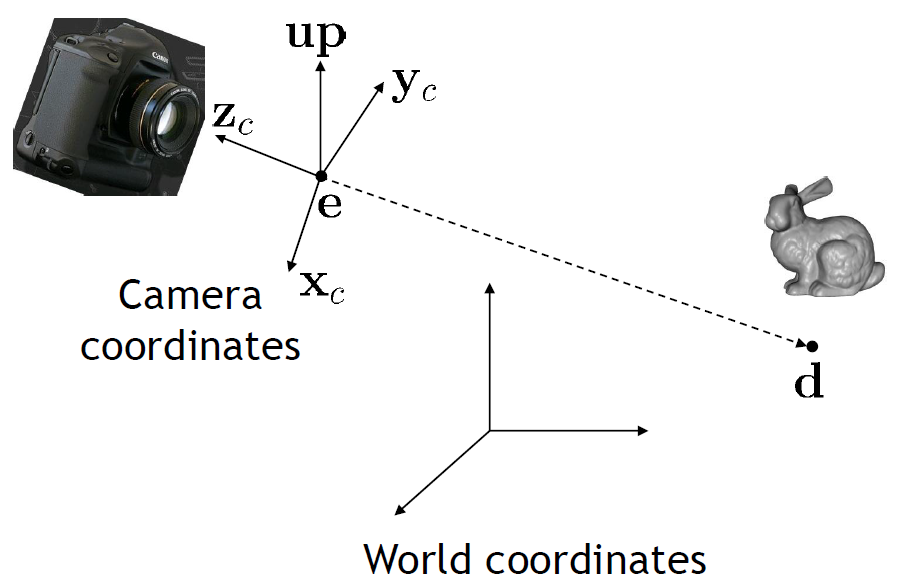
\includegraphics[scale=0.35]{implementation/cameramatrix.png}
  \caption[Camera Matrix]{Illustration$\footnotemark$ of involved components in order to construct the camera matrix $C$. The eye-vector $e$ denotes the positon of the camera in space, $d$ is the position the camera looks at, and $up$ denotes the cameras height. The camera space is spanned by the vectors helper vectors $x_c$, $y_c$ and $z_c$. Notice that objects we look at are in front of us, and thus have negative $z$ values}
  \label{fig:cameramatrix}
\end{figure}
\footnotetext{This image has been taken from the lecture slides of computer graphics class 2012 which can be found on ilias.}

The mathematical representation of these vectors, $x_c$, $y_c$ and $z_c$, spanning the camera space, introduced in figure $\ref{fig:cameramatrix}$, looks like the the following: 

\begin{align}
  &z_c = \frac{e-d}{||e-d||} \nonumber \\
  &x_c = \frac{up \times z_c}{||up \times z_c||} \nonumber \\
  &y_c = z_c \times x_c
  \label{eq:cameraspacespanningvectors}
\end{align}

As we can see, $x_c$, $y_c$ and $z_c$ are independent unit vectors. Therefore, they span a 3d space, the so called camera matrix. In order to express a coordinate in camera space, we have to project it onto these unit vectos. Using a homogenous coordinates representation, this a projection onto these unit vectors can be formulated by the transformation matrix $C$:
\begin{equation}
  C = \begin{bmatrix} x_c & y_c & z_c & e \\ 0 & 0 & 0 & 1 \end{bmatrix}
  \label{eq:cameramatrixeq}
\end{equation}

In our vertex shader, besides transforming the vertex positions like described in equation $\ref{eq:vertextransformation}$, for every vertex, we also compute the direction vectors $\omega_i$ and $\omega_r$ described like in figure $\ref{fig:geometricsetup}$. Those direction vectors are transformed onto the tangent space, a local coordinate system spanned by a vertex's normal, tangent and binormal vector. For further information and more insight about the the tangent space, please bave a look at the appendix in the section $\ref{sec:tangentspace}$. The algorithmic idea of our vertex shader, stating all its computational steps, is conceptualized in algorithm $\ref{alg:vertexshader}$.
  
\begin{algorithm}[H]
  \caption{Vertex diffraction shader pseudo code}
  \begin{algorithmic}
    \INPUT $Vertices,\ tranformation \ matrices,\ N,\ T,\ lightDir$
    \MOUTPUT $\omega_i,\ \omega_r,\ p_{per}$ 
      \ForAll{$Vertex \thinspace v \in Shape$}
        \State $ vec3 \ N = normalize(modelM * vec4(normal,0.0).xyz)$
        \State $ vec3 \ T = normalize(modelM * vec4(tangent,0.0).xyz)$
        \State $ vec3 \ B = normalize(cross(N, T))$
        \State $ TangentSpace = span(N, T, B)$
        \State $ vec3 \ Pos = ((cop_{w}-position)).xyz$
        \State $ lightDir = normalize(lightDir)$
        \State $ \omega_i = projectVectorOnTo(lightDir, TangentSpace)$
        \State $ \omega_r = projectVectorOnTo(Pos, TangentSpace)$
        \State $normalize(l); normalize(p)$
        \State $p_{per} = P \cdot C^{-1} \cdot M \cdot p_{obj}$
      \EndFor
      
  \end{algorithmic}
\label{alg:vertexshader}
\end{algorithm}

% brief description of algo steps
As an input For every vertex of a mesh

As already mentioned in section $\ref{sec:dirlighsourceassumption}$, our light source is a directional light source (See figure $\ref{fig:dirlightsource}$).

\begin{figure}[H]
  \centering
  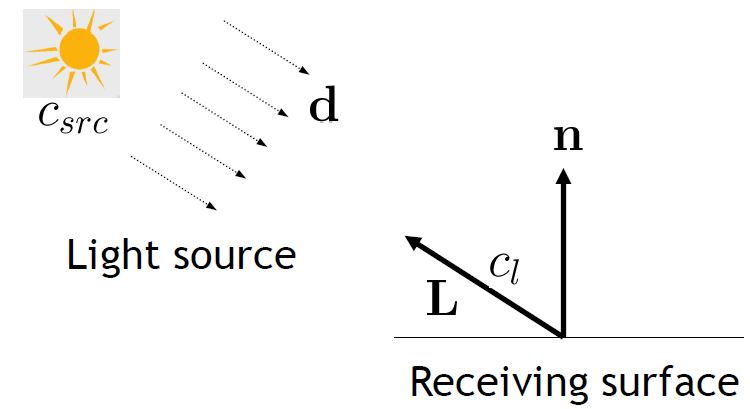
\includegraphics[scale=0.45]{implementation/dirlightsource.png}
  \caption[Rays of a Directional Light]{Illustration$\footnotemark$ of our light source setup. For a directional light source, all light rays are in parallel.}
  \label{fig:dirlightsource}
\end{figure}
\footnotetext{This image has been taken from the lecture slides of computer graphics class 2012 which can be found on ilias.}

\subsection{Fragment Shader}
\label{sec:fragmentshader}
The purpose of a fragment shader is to render per fragment. A fragment is spanned by three vertices of a given mesh. For each pixel within a fragment in the fragment shader, the output of from its spanning vertices computed in the vertex shaders $\ref{alg:vertexshader}$ is trilinearly interpolated depending on the pixel's position within the fragment. Furthermore, there can be additional input be assigned which is not directly interpolated from the output of vertex shader programs. In our fragment shader $\ref{alg:fragmentshaderall}$ this will be: all the references to the image buffers, containing the Fourier images computed in Matlab $\ref{sec:precompmatlabfourierimages}$, the number steps for the taylor approximation (in our shader 30), the minimal and maximal wavelength, scaling factors, a reference to a lookup table containing the $CIE_{XYZ}$ color weights. Basically the whole computation within our fragment shader relies on the direction of light and the viewing direction. Our shader performs a numerical integration for our final derived expression in equation $\ref{eq:finalexpression}$ using the trapezoidal-rule with uniform discretization of the wavelength spectrum at $5nm$ step sizes. This implies we are compressing sampled frequencies to the region near to the origin of their frequency domain due to the fact we are dividing the $(u,v)$ by the wavelength and this implies that the $(u,v)$ space is sampeled non-linearly. \\

The Gaussian window approach derived in section $\ref{sec:gaussianwindow}$ is performed for each discrete $\lambda$ value using a window large enough to span $4\sigma_f$ in both dimensions. For precomputing DFT tables we generally use nanostructure height fields that span at least 65$\mu m^2$ and are sampled with resolution of at least 100nm. This ensures that the spectral response encompasses all the wavelengths in the visible spectrum, i.e. from 380nm to 780nm.

\begin{algorithm}[H]
  \caption{Fragment diffraction shader pseudo code}
  \begin{algorithmic}[1]
    \INPUT $Precomputed \thinspace DFT \thinspace Terms,\thinspace Scene \thinspace Geometry$
    \MOUTPUT $Structural Color on Fragment$
    \ForAll{$Pixel \thinspace p \in Fragment$}
      \State \init $BRDF_{XYZ}, BRDF_{RGB}$ \myto $vec4(0.0)$
      \State $(u,v,w) = -\omega_i - \omega_r$
      \For{$(\lambda = \lambda_{min};\thinspace \lambda \leq \lambda_{max};\thinspace \lambda = \lambda + \lambda_{step})$}
        \State $xyzWeights = ColorWeights(\lambda)$
        \State $lookupCoord = lookupCoord(u, v, \lambda)$
        \State \init $P$ \myto $vec2(0.0)$
        \State $k = \frac{2\pi}{\lambda}$
        \For{$(n = 0$ \myto $T)$}
          \State $taylorScaleF = \frac{(kw)^n}{n!}$
          \State \init $F_{fft}$  \myto $vec2(0.0)$
          \State $anchorX = int(floor(center.x + lookupCoord.x * fftImWidth)$
          \State $anchorY = int(floor(center.y + lookupCoord.y * fftImHeight)$
          \For{$(i=(anchorX-winW)$ \myto $(anchorX + winW))$}
            \For{$(j=(anchorY - winW)$ \myto $(anchorY + winW))$}
              \State $dist = distVecFromOriginTo(i,j)$
              \State $pos = localLookUp(i,j,n)$
              \State $fftVal = rescaledFourierValueAt(pos)$
              \State $fftVal \asteq gaussWeightOf(dist)$
              \State $F_{fft} \pluseq fftVal$
            \EndFor
          \EndFor
          \State $P \pluseq taylorScaleF*F_{fft}$
        \EndFor
        \State $xyzPixelColor \pluseq dot(vec3(\left|P\right|^2), xyzWeights)$
      \EndFor
      \State $BRDF_{XYZ} = xyzPixelColor*C(\omega_i, \omega_r)*shadowF$
      \State $BRDF_{RGB}.xyz = D_{65}*M_{XYZ-RGB}*BRDF_{XYZ}.xyz$
      \State $BRDF_{RGB}= gammaCorrect(BRDF_{RGB})$
    \EndFor
  \end{algorithmic}
  \label{alg:fragmentshaderall}
\end{algorithm}


\myparagraph{From line 4 to 26:} 
This loop performs uniform sampling along wavelength-space. $ColorWeights(\lambda)$ computes the color weight for the current wavelength $\lambda$ by linear interpolation between the color weight for $\ceil{\lambda}$ and $\floor{\lambda}$ which are stored in a external weights-table (assuming this table contains wavelengths in 1nm steps). At line 6: $lookupCoord(u, v, \lambda)$ the coordinates for the texture lookup are computed - See $\ref{eq:scalelook}$. Line 25 sums up the diffraction color contribution for the current wavelength in iteration $\lambda$.  

\myparagraph{From line 9 to 24:} 
This loop performs the Taylor series approximation using T terms. Basically, the spectral response is approximated for our current $(u,v,\lambda)$. Furthermore, neighborhood boundaries for the gaussian-window sampling are computed, denoted as anchorX and anchorY.

\myparagraph{From line 14 to 22:} 
In this inner most loop, the convolution of the gaussian window with the DFT of the patch is performed. $gaussWeightOf(dist)$ computes the weights in equation $~\eqref{eq:gaussweight}$ from the distance between the current pixel's coordinates and the current neighbor's position in texture space. Local lookup coordinates for the current fourier coefficient $fftVal$ value are computed at line 17 and computed like described in $\ref{eq:gaussianwindowlook}$. The actual texture lookup is performed at line 18 using those local coordinates. Inside $rescaledFourierValueAt$ the values $fftVal$ is rescaled by its extrema, i,e. $(fftVal*Max + Min)$ is computed, since $fftVal$ is normalized $\ref{sec:precompmatlabfft}$. The current $fftVal$ values in iteration is scaled by the current gaussian weight and then summed to the final neighborhood FFT contribution at line 20.

\myparagraph{After line 26:} 
At line 27 the gain factor $C(\omega_i, \omega_r)$  $\ref{eq:cfact}$ is multiplied by the current computed pixel color like formulated in $\ref{eq:cpterm}$. The gain factor contains the geometric term $ref{eq:geometricterm}$ and the Fresnel term $F$. W approximate $F$ by the Schlick approximation $\ref{eq:schlickapprox}$, using an reactive index at 1.5 since this is close to the measured value from snake sheds.
Our BRDF values are scaled by s shadowing function as described in (SEE REFERENCES - PAPER), since most of the grooves in the snake skin nano-structures would from a V-cavity along the plane for a wave front with their top-edges at almost the same height.

Last, we transform our colors from the $CIE_XYZ$ colorspace to the $CIE_RGB$ space using the CIE Standard Illuminant D65, followed by a gamma correction. See $\ref{subsec:colortransformations}$ for further insight.

\section{Technical details}
\subsection{Texture lookup}
In a GLSL shader the texture coordinates are normalized which means that the size of the texture maps to the coordinates on the range $[0,1]$ in each dimension. By convention the the bottom left corner of an image has the coordinates $(0,0)$, whereas the top right corner has the value $(1,1)$ assigned. 

Given a nano-scaled surface patch P with a resolution $A$ by $A$ microns stored as an $N$ by $N$ pixel image $I$.
Then one pixel in any direction corresponds to $dH = \frac{A}{N} \mu m$. 
In Matlab we compute a series of $n$ output images $\{I_{out_1},...,I_{out_n}\}$ from $I$, which we will use for the lookup in our shader - See figure $\ref{fig:lookupexample}$. For the lookup we use scaled and shifted $(u,v)$ coordinates from $\ref{eq:uvw}$. 

Since the zero frequency component of output images was shifted towards the centre of each image, we have to shift $u$, $v$ to the center of the current $N$ by $N$ pixel image by a bias $b$. Mathematically, the bias is a constant value is computed the following:

\begin{align}
    b
    &= (N \% 2 == 0) \quad ? \quad \frac{N}{2} : \frac{N-1}{2}
\label{eq:bias}
\end{align}

\begin{figure}[H]
  \centering
  \includegraphics[scale=0.7]{implementation/lookupexampleAmReIm4.png}
  \caption[Lookup in DFT Terms]{$(u,v)$ lookup image}
\label{fig:lookupexample}
\end{figure}

For the scaling we have to think a little further: lets consider a $T$ periodic signal in time, i.e. $x(t) = x(t+nT)$ for any integer n. After applying the DFT, we have its discrete spectrum $X[n]$ with frequency interval $w0 = 2pi / T$ and time interval $t0$. Let $k = \frac{2 \pi}{\lambda}$ denote the wavenumber for the current wavelength $\lambda$.
Then the signal is both periodic with time period $T$ and discrete with time interval $t_0$ then its spectrum should be both discrete with frequency interval $w_0$ and periodic with frequency period $\Omega = \frac{2 \pi}{t_0}$. This gives us the idea how to discretize the spectrum: Let us consider our Patch $P$ assuming it is distributed as a periodic function on our surface. Then, its frequency interval along the x direction is $w_0 = \frac{2 \pi}{T} = \frac{2 \pi}{N*dH}$. 
Thus only wave numbers that are integer multiples of $w_0$ after a multiplication with $u$ must be considered, i.e. $ku$ is integer multiple of $w_0$. Hence the lookup for the u-direction will look like:

\begin{align}
    \frac{ku}{w_0} 
    &= \frac{ku N dH}{2 \pi} \\
    &= \frac{u N dH}{\lambda}
\label{eq:scalelook}
\end{align}

Using those findings $\ref{eq:bias}$, $\ref{eq:scalelook}$, the final $(u,v)$ texture lookup-coorinates for the current wavelength $\lambda$ in iteration, will then look like:

\begin{equation}
  (u_{lookup}, v_{lookup}) = \left( \frac{u N dH}{\lambda} + b, \frac{v N dH}{\lambda} + b \right)
\label{eq:ublookup}
\end{equation}  

Note for the windowing approach we are visiting a one pixel neighborhood for each pixel $p$. 
This is like a base change with $(u_{lookup}, v_{lookup})$ as new coordinate system origin. The lookup coordinates for the neighbor-pixel $(i,j)$ are:

\begin{equation}
  (u_{lookup}, v_{lookup}) = (i,j)-(u_{lookup}, v_{lookup})
\label{eq:gaussianwindowlook}
\end{equation}

\subsection{Texture Blending}
The final rendered color for each pixel is a weighted average of different color components, such as the diffraction color, the texture color and the diffuse color. In our shader the diffraction color is weighted by a constant $w_{diffuse}$. the texture color is once scales by a binary weight determined by the absolute value of the Fresnel Term $F$ and once by $1-w_{diffuse}$. 

\begin{algorithm}[H]
  \caption{Texture Blending}
  \begin{algorithmic}
    \State $\alpha = (abs(F) > 1) ? 1 : 0$
    \State $c_{out} =(1-w_{diffuse})*c_{diffraction} + (1-\alpha)*c_{texture} + w_{diffuse}*c_{texture})$
  \end{algorithmic}
\end{algorithm}

\subsection{Color Transformation}
\label{subsec:colortransformations}

In our shader we access a table which contains precomputed CIE's color matching functions values from $\lambda_{min} = 380 nm$ to $\lambda_{max} = 780 nm$ in $5 nm$ steps. Such a function value table can be found at downloaded at cvrl.ioo.ucl.ac.uk for example. We compute the $(X,Y,Z)$ $CIE_{XYZ}$ color values as described in section $\ref{sec:colorspace}$. 


We can transform the color values into $CIE_{RGB}$ by performing the following linear transformation:

\begin{equation}
\begin{bmatrix}R\\G\\B\end{bmatrix} = M \cdot \begin{bmatrix}X\\Y\\Z\end{bmatrix}
\end{equation} 

where one possible transformation is: 

\begin{equation}
M = \begin{bmatrix} 0.41847 & -0.15866 & -0.082835\\ -0.091169 & 0.25243 & 0.015708\\ 0.00092090 & -0.0025498 & 0.17860 \end{bmatrix}
\end{equation}

There are some other color space transformation. The shader uses the CIE Standard Illuminant D65 which is intended to represent average daylight. Using D65 the whole colorspace transformation will look like:

\begin{equation}
\begin{bmatrix}R\\G\\B\end{bmatrix} = M \cdot \begin{bmatrix}X \cdot D65.x \\ Y \cdot D65.y \\Z \cdot D65.z \end{bmatrix} 
\end{equation}

Last we perfrom gamma correction on each pixel's $(R,G,B)$ value. Gamma correction is a non linear transformation which controls the overall brightness of an image.

\section{Discussion}
\label{sec:impldiscus}
The fragment shader algorithm described in $\ref{alg:fragmentshaderall}$ performs the gaussian window approach by sampling over the whole wavelength spectrum in uniform step sizes. This algorithm is valid but also slow since we iterate for each pixel over the whole lambda spectrum. Furthermore, for any pixel, we iterate over its 1 neighborhood. Considering the loop for the taylor approximation as well, we will have a run-time complexity of $O(\#spectrtumIter \cdot \#taylorIter \cdot neighborhoodRadius^2)$. 
Hence, Instead sampling over the whole wavelength spectrum, we could instead integrate over just a few required lambdas which are elicited like the following: Lets consider $(u,v,w)$ defined as $\ref{eq:uvw}$. Let $d$ be the spacing between two slits of a grating. For any $L(\lambda) \neq 0$ it follows $\lambda_{n}^{u} = \frac{d u}{n}$ and $\lambda_{n}^{v} = \frac{d u}{n}$. For $n = 0$ there it follows $(u,v)=(0,0)$. 
If $u,v > 0$
\begin{align*}
    N_{min}^{u} = \frac{d u}{\lambda_{max}} \leq n_{u} \leq \frac{d u}{\lambda_{min}} = N_{min}^{u}\\
    N_{min}^{v} = \frac{d v}{\lambda_{max}} \leq n_{v} \leq \frac{d v}{\lambda_{min}} = N_{min}^{v}
\end{align*}
If $u,v < 0$
\begin{align*}
    N_{min}^{u} = \frac{d u}{\lambda_{min}} \leq n_{u} \leq \frac{d u}{\lambda_{min}} = N_{max}^{u}\\
    N_{min}^{v} = \frac{d v}{\lambda_{min}} \leq n_{v} \leq \frac{d v}{\lambda_{min}} = N_{max}^{v}
\end{align*}

By transforming those equation to $(\lambda_{min}^{u}, \lambda_{min}^{u})$, $(\lambda_{min}^{v}, \lambda_{min}^{v})$ respectively for any $(u,v,w)$ for each pixel we can reduce the total number of required iterations in our shader.  

Another variant is the $PQ$ approach described in chapter 2 $\ref{sec:pq}$. Depending on the interpolation method, there are two possible variants we can think of as described in $\ref{sec:sincinterpolation}$. Either we try to interpolate linearly or use sinc interpolation.
The first variant does not require to iterate over a pixel's neighborhood, it is also faster than the gaussian window approach. One could think of a combination of those tho optimization approaches. Keep in mind, both of these approaches are further approximation. The quality of the rendered images will suffer using those two approaches. The second variant, using the sinc function interpolation is well understood in the field of signal processing and will give us reliable results. The drawback of this approach is that we again have to iterate over a neighborhood within the fragment shader which will slow down the whole shading. The following algorithm describes the modification of the fragment shader  $\ref{alg:fragmentshaderall}$ in oder to use sinc interpolation for the PQ approach $\ref{sec:pq}$.  

\begin{algorithm}[H]
  \caption{Sinc interpolation for PQ approach}
  \begin{algorithmic}
    \ForAll{$Pixel \thinspace p \in Image \thinspace I$}
      \State $w_p = \sum_{(i,j) \in \mathcal{N}_{1}(p)} sinc(\Delta_{p,(i,j)} \cdot \pi + \epsilon) \cdot I(i,j)$
      \State $c_p = w_p \cdot (p^2 + q^2)^{\frac{1}{2}}$
      \State $render(c_p)$
    \EndFor
  \end{algorithmic}
  \label{alg:sincinterpolation}
\end{algorithm}

In a fragment shader we compute for each pixel $p$ in the current fragment its reconstructed function value $f(p)$ stores in $w_p$. $w_p$ is the reconstructed signal value at $f(p)$ by the sinc function as described in $\ref{sec:sincinterpolation}$.
We calculate the distance $\Delta_{p,(i,j)}$ between the current pixel $p$ and each of its neighbor pixels $(i,j) \in \mathcal{N}_{1}(p)$ in its one-neighborhood. Multiplying this distance by $\pi$ gives us the an angle used for the sinc function interpilation. We add a small integer $\epsilon$ in order to avoid division by zeros side-effects.


% \newpage{\pagestyle{empty} \cleardoublepage}
% 
% \chapter{Evaluation Data Acquisition}
\section{Data Acquisition}
For measurement on the true surface topography of snake sheds, samples are stuck on glass plates using double face tape, the animal was pushed up below a hollowed plate letting the skin emerging from the top of the plate using an atomic force microscope (AFM). An AFM is a microscope that uses a tiny probe mounted on a cantilever to scan the surface of an object. The probe is extremely close tobut does not touch the surface. As the probe traverses the surface, attractive and repulsive forces arising between it and the atoms on the surface induce forces on the probe that bend the cantilever. The amount of bending is measured and recorded, providing a map of the atoms on the surface. Atomic force microscopes is a very high-resolution type of scanning probe microscopy, with demonstrated resolution on the order of fractions of a nanometer, more than 1000 times better than the optical diffraction limit.

\section{Diffraction Gratings}
An idealised grating like in figure $\ref{fig:lighthitsgrating}$ is made of a very large number of parallel, evenly spaced slits in an opaque sheet. Typically, it would have about 10,000 slits. In order to cause diffraction, the spacing between slits must be wider than the wavelength of the incoming light beam. Each slit in the grating acts as a quasi point light source from which light propagates in all directions. Figure $\ref{fig:spectometer}$ illustrates this behaviour for a monochromatic light source passing through a grating and shows that the the outgoing angle will be different from the incident angle. Hence, the diffracted light $\ref{diffractiondeff}$ is composed of the sum of interfering wave components emanating from each slit in the grating.

\begin{figure}[H]
  \centering
  \includegraphics[scale=0.7]{evaluation/spectrometer.jpg}
  \caption{Spectometer: When a beam of monochromatic light passes through a grating placed in a spectrometer, images of the sources can be seen through the telescope at different angles.}
\label{fig:spectometer}
\end{figure}

Suppose monochromatic light is directed at the grating parallel to its axis as shown in figure $\ref{fig:spectometer}$. Let the distance between successive slits be equal $d$.

\begin{figure}[H]
  \centering
  \includegraphics[scale=0.7]{evaluation/grating2.jpg}
  \caption{Light directed to parallel to grating:}
  \label{fig:lighthitsgrating}
\end{figure}

The diffraction pattern on the screen is the result of the combined effects of diffraction and interference. Each slit causes diffraction, and the diffracted beams in turn interfere with one another to produce the pattern. The path difference between waves from any two adjacent slits can be found by dropping a perpendicular line between the parallel waves. By geometry, this path difference is $d sin(\theta)$. If the path difference equals one wavelength or some integral multiple of a wavelength, waves from all slits will be in phase and a bright line will be observed at that point. Therefore, the condition for maxima in the interference pattern at the angle $\theta$ is: 

\begin{equation}
 d sin(\theta) = m \lambda 
\label{eq:simplegratingequation}
\end{equation}

where $m \in \mathds{N}_0$ is the order of diffraction.

Because $d$ is very small for a diffraction grating, a beam of monochromatic light passing through a diffraction grating is splitted into very narrow bright fringes at large angles $\theta$.

\begin{figure}[H]
  \centering
  \includegraphics[scale=0.7]{evaluation/GratingSurface.png}
  \caption{Different Orders of diffraction}
\label{fig:gratingdiffractionorders}
\end{figure}

When a narrow beam of white light is directed at a diffraction grating along its axis, instead of a monochromatic bright fringe, a set of colored spectra are observed on both sides of the central white band as shown in figure $\ref{fig:gratingdiffractionorders}$.

\begin{figure}[H]
  \centering
  \includegraphics[scale=0.7]{evaluation/coloredspectrum.jpg}
  \caption{White Light beam causes coloured diffraction spectra}
  \label{fig:diffractionSpectrum}
\end{figure}

Since the angle $\theta$ increases with wavelength $\lambda$, red light, which has the longest wavelength, is diffracted through the largest angle. Similarly violet light has the shortest wavelength and is therefore diffracted the least. This relationship between angle and wavelength is illustrated in figure $\ref{fig:diffractionSpectrum}$. Thus, white light is split into its component colors from violet to red light. The spectrum is repeated in the different orders of diffraction, emphasizing certain colors differently, depending on their order of diffraction like shown in figure $\ref{fig:gratingdiffractionorders}$. Note that only the zero order spectrum is pure white.  
Figure $\ref{fig:nslitdiffractionintensity}$ shows the relative intensity resulting when a beam of light hits a diffraction grating for different number of periods. From the graph we recognise that the more slits a grating has, the sharper more slopes the function of intensity gets. This is similar like saying that, the more periods a grating has, the sharper the diffracted color spectrum gets like shown in figure $\ref{fig:diffractionslits}$. 

\begin{figure}[H]
  \centering
  \includegraphics[scale=0.35]{evaluation/nslitdiffraction.png}
  \caption{Relative intensitiies of a diffracted beam of light at wavelength $\lambda=500nm$ on a grating for different number of periods $N$ width slit width of 30 microns and slit seperation of 0.15 mm each. The viewer is 0.5m apart from the grating.}
  \label{fig:nslitdiffractionintensity}
\end{figure}

\begin{figure}[H]
  \centering
  \subfigure[one slit]{
    \includegraphics[scale=0.2]{evaluation/slits/spalt1.png}
    \label{fig:diffractionSlits1}
  }

~
  \subfigure[seven slits]{
    \includegraphics[scale=0.2]{evaluation/slits/spalt07.png}
    \label{fig:diffractionSlits7}
  }
  
  
  \caption{Difference of diffraction pattern between a monochromatic (top) and a white (bottom) light spectra for different number of slits.}
\label{fig:diffractionslits}
\end{figure}

\section{Evaluation}

\begin{figure}[H]
  \centering
  \includegraphics[scale=0.65]{evaluation/evalsetup.png}
  \caption{Experimental setup for evaluation: A light beam with direction $L$ hits the surface, representing a grating pattern with periodicity $d$, at the incident plane relative to the surface normal $n$ at angle $\theta$ and emerges at angle $\phi$ with direction $V$.}
  \label{fig:experimentalsetup}
\end{figure}

The physical reliability of our BRDF models has been verified by applying those on various patches which are a synthetic blazed grating, an Elaphe and a Xenopeltis snake shed sample patch. We compared the resulting response against the response resulting by the grating equation, which models the relationship between the grating spacing and the angles of the incident and diffracted beams of light. Figure $\ref{fig:experimentalsetup}$ illustrates the geometrical setup for our evaluation approach: A monochromatic beam of light with wavelength $\lambda$ hits a surface with periodicity $d$ at an angle $\theta$ relative to the normal $n$ along its incident plane. The beam emerges from the surface at the angle $\phi$. 

\begin{figure}[H]
  \centering
  \includegraphics[scale=0.45]{evaluation/reflgrating.png}
  \caption{Reflecting grating: When the incident light direction is not parallel to its axis at the grating, there is another $sin(\phi)$ involved. See also the grating equation $\ref{eq:gratingeq}$.}
  \label{fig:reflgrating}
\end{figure}

The maximum in intensity is given by the grating equation derived from the equation $\ref{eq:simplegratingequation}$ following figure $\ref{fig:reflgrating}$: 

\begin{equation}
  sin(\theta) = sin(\phi) + \frac{m \lambda}{d}
\label{eq:gratingeq}
\end{equation}

In our evaluation we are interested in the first order diffraction, i.e. m equals one which. We further assume that the incident light direction $w_i$ is given. In contrast the direction of the reflected wave $w_r$ is not given.
In Mathematics, a three dimensional direction vector is fully defined by two two angles, i.e. it can be represented by spherical coordinates with radius $r = 1$. By convention, we denote those two vectors by $\theta$ and $\phi$. Hence, $\theta_i$, $\phi_i$ and $\phi_r$ are given constants whereas $\theta_i$ is a free parameter for our evaluation simulation. Therefore, we are going to compare the maxima for peak viewing angle corresponding to each wavelength using data produced by our method against the maxima resulting by the grating equation.

\subsection{Precomputation}
For evaluation purposes we have implemented our brdf models in java. We once again use our geometrical setup as illustrated in figure $\ref{fig:geometricsetup}$ where $\theta_i$, $\phi_i$ and $\phi_r$ are provided as input values and $\theta_i$ is a free parameter. Within our evaluation we have set them to $\theta_i = 75$ $\phi_i = 0$ $\phi_r = 180$ degrees. The wavelength space $\Lambda$ and the range $\Theta$ of our free parameter $\theta_i$ are discretized in equidistant steps whereas their steps sizes are given as input arguments of our java program:

\begin{equation}
\Lambda = \{\lambda | \lambda = \lambda_{min} + k \cdot \lambda_{step}, \quad k \in \{0,..,C-1\}\}
\label{eq:lambdaspacesetup}
\end{equation}

where $\lambda_{step} = \frac{\lambda_{max}-\lambda_{min}}{C-1}$ and $C$ is the discretisation level of the lambda space, in our scenario $C = 42$. We similarly discretise the angle space by predefining an minimal and maximal angle boundary and $ceil(angMax - angMin) / angInc$ is the number of angles. Our java brdf model implementations are applied on the grid $[\Lambda, \Theta]$ and will store their spectral response in a matrix

\begin{equation} 
R = \{response(\lambda_i, \theta_{r}^{j}) | i \in Index(\Lambda), \quad j \in Index(\Theta)\}
\label{eq:responsematrix}
\end{equation}

We will plot this matrix and compare its graph against the grating equation for similar condition like in stated in algorithm $\ref{alg:evalmatlab}$.

\begin{algorithm}[H]
  \caption{Vertex diffraction shader}
  \begin{algorithmic}
    \State{load matrix $R$ $\ref{eq:responsematrix}$}
    \State $ \lambda_{count} = |\Lambda| $
    \State $ \lambda_{inc} = \frac{\lambda_{max}-\lambda_{min}}{\lambda_{count}}$
    \State $ \lambda = \lambda_{min} + \lambda_{inc} \cdot (-1+[1:\lambda_{count}])$
    \State $ [maxC maxI] = max(R)$
    \State $ viewAngForMax = angMin + angInc \cdot (maxI-1)$
    \State $ thetaV = asin \left( \frac{\lambda}{d} - \sin \left(  \frac{\theta_I \pi}{180} \right) \right) \cdot \frac{180}{\pi}$
    \State $ plot(\lambda, viewAngForMax)$
    \Comment{graph resulting by our brdf model}
    \State $ plot(lambda, thetaV)$
    \Comment{graph resulting by grating equation}
  \end{algorithmic}
\label{alg:evalmatlab}
\end{algorithm}

\subsection{Data evaluation}

\begin{figure}[H]
  \centering
  \subfigure[Blaze grating]{
    \includegraphics[scale=0.42]{evaluation/blazeHR.png}
    \label{fig:blazeval}
  }
~
  \subfigure[Xenopeltis]{
    \includegraphics[scale=0.42]{evaluation/XenoHR.png}
    \label{fig:xenopeltiseval}
  }
~
\subfigure[Elaphe]{
  \includegraphics[scale=0.75]{evaluation/ElapheHR.png}
  \label{fig:elapheeval}
}

  \caption{Reflectance obtained by using the shading approach described in algorithm $\ref{alg:fragmentshaderall}$ simulating a BRDF which models the effect of diffraction at different viewing angles over the spectrum of visible light.}

\label{fig:evaluationdiffshaderalllambda}
\end{figure}

Figure $\ref{fig:evaluationdiffshaderalllambda}$ shows fits of angles for first order diffraction of an idealized periodic structure using an illumination angle $\theta = 75$ degrees. The graphs $\ref{fig:elapheeval}$ and $\ref{fig:elapheeval}$ in figure $\ref{fig:evaluationdiffshaderalllambda}$ show reflectance of different nano-scaled structures computed by the uniform wavelength sampling fragment shader described as in algorithm $\ref{alg:fragmentshaderall}$. Higher values are in yellow, lower values in green. Viewing angles for peak reflectances of the nanostructues at each wavelength (red curve) and diffraction angles for an idealized periodic structure with a certain periodicity $d$ according to the grating equation $\ref{eq:gratingeq}$.

For each of the graphs we determine the vieweing angles with peak reflectance for various wavelengths and then plot this peak viewing angles against their wavelength as solid red curves. This red curve closely matches the blue curve representing the grating equation with the value of a edstimated from the peak view angles, listed in external source.


since blazed grating is synthetic we use its exact periodicity to plot the blue curve instead of estimating it. xeno evaluated just along the direction for the finger like structures.

the red and blue curve are closely overlapping in our figures $\ref{fig:blazeval}$ and $\ref{fig:elapheeval}$. For blaze and elaphe there is only diffraction along only along one direction perceivable.

for xeno its interesting to see that the red curve for the peak viewing angle toggles between two ridges correspinding to two different periodicities. this happens because there are multiple sub regions of the nanostructure whith slithly different orientations and periodicit. Each sub region carves out a different yellowish ridge. depending on the viewing agnle, reflectance due to one such subregion can be higher than from the others.




subvariants: sample whole lambda space, just a few lambdas, pq approach.
discussion

% \newpage{\pagestyle{empty} \cleardoublepage}
% % 
\chapter{Results}

show comparision between all shader variants: pq, adaptive, all, nvidiaGem.
mention system specs and how long it took in order to precompute
mention GEM results.
show nminmax renderings










Mention basic set up


brdf map for blazed grating shows typical high relative brightness for the first order of diffraction.

elaphe skin, finger-like nanostructure quite regularly placed, thus exhibits diffraction accros these periodic arrangements, i.e. there is a long horizontal axis for brdf map. furthermore fingers overlap across layers thus do not exhibit any definite periodicity along finger directions. hence do not see strong diffraction color along other directions in brdf map.

for xeno, layers of nano-fingers do not overlap and they manoeuvre significantly along their lenght but with some local consistency. thus see diffraction along many different directions in brdf map. similar argument for diffraction across locally periodic finger patches with slightly different orientations.


the elapse does not look that regular under the electron scanning microscope. This is why it is much less iridescent than the other specie.

In addition, the micro-geometry is highly similar among snake species, it is the geometry of the nanostructures that are highly different among species and that cause the snake to be or not be iridescent. So, even Xenopeltis would not give you very different geometry than Elaphe.

Xeno has a brownish body with no pattern that makes the iridescence more spectacular than on Ellaphe


\section{BRDF maps}
In this chapter we examine the rendered output resulting by the implementation of our BRDF models applied on different input patches such as Blaze grating or Elaphe $\ref{fig:elpahespecies}$ and Xenopeltis $\ref{fig:xenospeicies}$ snake nano-scaled surface sheds. We going to discuss and compare both, their BRDF maps $\ref{fig:brdfmapexplanation}$ and the corresponding renderings on a snake geometry $\ref{sec:snakegeomrenderings}$ for various input parameters. Last we also show a real experimental image showing the effect of diffraction for similar parameters like we have. 
A BRDF map shows a shader's output for all possible viewing directions for a given, fixed, incident light direction. We assume that each viewing direction is in spherical coordinates form $\ref{sec:sphericalcoordinates}$ $(\theta_v, \phi_v)$ and is represented in the map at point $(x,y) = (sin(\theta_v)cos(\phi_v), sin(\theta_v)sin(\phi_v))$ with its origin at the map-center. The light direction for normal incidence $(\theta_i, \phi_i)$ has been fixed to $(0,\pi)$ for our rendered results.

\begin{figure}[H]
  \centering
  \subfigure[BRDF map schema]{
    \includegraphics[scale=0.53]{results/brdfmapschema.png}
    \label{fig:brdfmapschema}
  }
~
  \subfigure[Light reflection geometrical setting]{
    \includegraphics[scale=0.68]{results/Lightreflectiongeometry.png}
    \label{fig:lightreflectiongeometry}
  }
~

\caption{BRDF maps for different patches: $\Theta=(\theta,\phi)$ is the direction of light propagation}
\label{fig:brdfmapexplanation}
\end{figure}

In this chapter we examine the rendered output resulting by the implementation of our BRDF models applied on different input patches $\ref{fig:gratingpatches}$ such as Blaze grating or Elaphe $\ref{fig:elpahespecies}$ and Xenopeltis $\ref{fig:xenospeicies}$ snake nano-scaled surface sheds. We going to discuss and compare both, their BRDF maps $\ref{fig:brdfmapexplanation}$ and the corresponding renderings on a snake geometry $\ref{sec:snakegeomrenderings}$ for various input parameters. Last we also show a real experimental image showing the effect of diffraction for similar parameters like we have. 
A BRDF map shows a shader's output for all possible viewing directions for a given, fixed, incident light direction. We assume that each viewing direction is in spherical coordinates form $\ref{sec:sphericalcoordinates}$ $(\theta_v, \phi_v)$ and is represented in the map at point $(x,y) = (sin(\theta_v)cos(\phi_v), sin(\theta_v)sin(\phi_v))$ with its origin at the map-center. The light direction for normal incidence $(\theta_i, \phi_i)$ has been fixed to $(0,\pi)$ for our rendered results.

\begin{figure}[H]
  \centering
  \subfigure[Blaze grating with scale of 2.500 $\mu m$]{
    \includegraphics[scale=0.5]{evaluation/blaze_res.png}
    \label{fig:blazegratingpatch}
  }
~
  \subfigure[Elaphe patch with scale of 3.270 $\mu m$]{
    \includegraphics[scale=0.5]{evaluation/elaphe_res.png}
    \label{fig:elpahegratingpatch}
  }
~
  \subfigure[Cenopeltis patch with scale of 3.210 $\mu m$]{
    \includegraphics[scale=0.5]{evaluation/xeno_res.png}
    \label{fig:xenogratingpatch}
  }

\caption{Cutouts of our nano-scaled surface gratings used for rendering within our shader with a scale indicator (red line) for each patch. Note that for rendering we use larger patches.}
\label{fig:gratingpatches}
\end{figure}


Figure $\ref{fig:brdfmapsdiffpatches}$ shows the BRDF maps of the full lambda space sampling approach $\ref{sec:fragmentshader}$ applied on different nanoscale surface gratings as shown in figure $\ref{fig:gratingpatches}$.

% brdf maps patches
\begin{figure}[H]
  \centering
  \subfigure[Blaze grating]{
    \includegraphics[scale=0.12]{results/diffPatches/fftBlazeHeight_0.25Microns_allL_weak_scale.png}
    \label{fig:brdfmapBlaze}
  }
~
  \subfigure[elaphe grating]{
    \includegraphics[scale=0.12]{results/diffPatches/elaph65.png}
    \label{fig:brdfmapElaphe}
  }
~
  \subfigure[xeno grating]{
    \includegraphics[scale=0.12]{results/diffPatches/xeno65.png}
    \label{fig:brdfmapXeno}
  }

\caption{BRDF maps for different patches}
\label{fig:brdfmapsdiffpatches}
\end{figure}

Figure $\ref{fig:brdfmapsdiffrenderingapproaches}$ shows the BRDF maps of all our BRDF models applied on the Blaze grating.
CHANGE PQ, N MIN MAX IMAGE SINCE SINC INTERPOL IS MISSING

% brdf maps patches
\begin{figure}[H]
  \centering
  \subfigure[ALL lambda]{
    \includegraphics[scale=0.09]{results/diffPatches/fftBlazeHeight_0.25Microns_allL_weak_scale.png}
    \label{fig:brdfmapBlazeAllLambda}
  }
~
  \subfigure[Nmin Nmax]{
    \includegraphics[scale=0.09]{results/methodComp/gem.png}
    \label{fig:brdfmapBlazeOnlyReq}
  }
~
  \subfigure[PQ]{
    \includegraphics[scale=0.09]{results/PQapproach_vs_sampleAll/blaze/pq.png}
    \label{fig:brdfmapBlazePQ}
  }
~
  \subfigure[Gem]{
    \includegraphics[scale=0.09]{results/methodComp/gem.png}
    \label{fig:brdfmapBlazeGem}
  }
    
\caption{BRDF maps for Blaze grating comparing our different rendering apporaches}
\label{fig:brdfmapsdiffrenderingapproaches}
\end{figure}

% add also a comp. for elaphe

Figure $\ref{fig:brdfmapsdifflambdastepsblaze}$ and figure $\ref{fig:brdfmapsdifflambdastepselaphe65}$ show the BRDF maps for different wavelength step sizes used in the fragment shader for the full lambda space sampling approach applied on the Blaze grating and the Elpahe snake shed, respectively.  

wider steps fewer iterations, loss of qulatiy. for elaphe step bigger than 10nm there are visible artifacts. for blaze grating bigger step sizes possible. 
% blaze steps
\begin{figure}[H]
  \centering
  \subfigure[$\lambda_{step=1 nm}$]{
    \includegraphics[scale=0.12]{results/different_lambda_steps/blaze/dl=1.png}
    \label{fig:brdfmapsDiffLambdaStepsL1Blaze}
  }
~
  \subfigure[$\lambda_{step=5 nm}$]{
    \includegraphics[scale=0.12]{results/different_lambda_steps/blaze/dl=5.png}
    \label{fig:brdfmapsDiffLambdaStepsL5Blaze}
  }
~
  \subfigure[$\lambda_{step=10 nm}$]{
    \includegraphics[scale=0.12]{results/different_lambda_steps/blaze/dl=10.png}
    \label{fig:brdfmapsDiffLambdaStepsL10Blaze}
  }
  
  \subfigure[$\lambda_{step=25 nm}$]{
    \includegraphics[scale=0.12]{results/different_lambda_steps/blaze/dl=25.png}
    \label{fig:brdfmapsDiffLambdaStepsL25Blaze}
  }
~
  \subfigure[$\lambda_{step=50 nm}$]{
    \includegraphics[scale=0.12]{results/different_lambda_steps/blaze/dl=50.png}
    \label{fig:brdfmapsDiffLambdaStepsL50Blaze}
  }
~ 
  \subfigure[$\lambda_{step=100 nm}$]{
    \includegraphics[scale=0.12]{results/different_lambda_steps/blaze/dl=100.png}
    \label{fig:brdfmapsDiffLambdaStepsL100Blaze}
  }
  
\caption{Blaze grating at $2.5 \mu m$: Different $\lambda$ step sizes}
\label{fig:brdfmapsdifflambdastepsblaze}
\end{figure}

% elpahe steps
\begin{figure}[H]
  \centering
  \subfigure[$\lambda_{step=1 nm}$]{
    \includegraphics[scale=0.12]{results/different_lambda_steps/elaphe65/dl=1.png}
    \label{fig:brdfmapsDiffLambdaStepsL1Elaphe65}
  }
~
  \subfigure[$\lambda_{step=5 nm}$]{
    \includegraphics[scale=0.12]{results/different_lambda_steps/elaphe65/dl=5.png}
    \label{fig:brdfmapsDiffLambdaStepsL5Elaphe65}
  }
~
  \subfigure[$\lambda_{step=10 nm}$]{
    \includegraphics[scale=0.12]{results/different_lambda_steps/elaphe65/dl=10.png}
    \label{fig:brdfmapsDiffLambdaStepsL10Elaphe65}
  }
  
  \subfigure[$\lambda_{step=25 nm}$]{
    \includegraphics[scale=0.12]{results/different_lambda_steps/elaphe65/dl=25.png}
    \label{fig:brdfmapsDiffLambdaStepsL25Elaphe65}
  }
~
  \subfigure[$\lambda_{step=50 nm}$]{
    \includegraphics[scale=0.12]{results/different_lambda_steps/elaphe65/dl=50.png}
    \label{fig:brdfmapsDiffLambdaStepsL50Elaphe65}
  }
~ 
  \subfigure[$\lambda_{step=100 nm}$]{
    \includegraphics[scale=0.12]{results/different_lambda_steps/elaphe65/dl=100.png}
    \label{fig:brdfmapsDiffLambdaStepsL100Elaphe65}
  }
  
\caption{Elaphe grating at $65 \mu m$: Different $\lambda$ step sizes}
\label{fig:brdfmapsdifflambdastepselaphe65}
\end{figure}


The Figures $\ref{fig:pqblaze}$, $\ref{fig:pqxeno}$, $\ref{fig:pqelaphe}$ show a comparison of the BRDF maps produced by full lambda space sampling approach (on the left) and the PQ shading approach (on the right) applied on all our patches. 
see similarities but also differences RERENDER PQ

%pq blaze
\begin{figure}[H]
  \centering
  \subfigure[Full Lambda Sampling: Blaze grating]{
    \includegraphics[scale=0.12]{results/PQapproach_vs_sampleAll/blaze/fftBlazeHeight_0.25Microns_allL_weak_scale_g=1.1.png}
    \label{fig:fullLambdaBlaze}
  }
~
  \subfigure[Full Lambda Sampling brightened: Blaze grating]{
            \includegraphics[scale=0.12]{results/PQapproach_vs_sampleAll/blaze/fftBlazeHeight_0.25Microns_allL_weak_scale_g=2.2_scale=100.png}
    \label{fig:fullLambdaBrightenedBlaze}
  }
~
  \subfigure[PQ Approach: Blaze grating]{
    \includegraphics[scale=0.12]{results/PQapproach_vs_sampleAll/blaze/pq.png}
    \label{fig:pqBlaze}
  }
  
\caption{Blaze grating: PQ approach vs full lambda space sampling}
\label{fig:pqblaze}
\end{figure}

%pq xeno
\begin{figure}[H]
  \centering
  \subfigure[Full Lambda Sampling: Xeno grating $\theta_i = 0 degree$]{
    \includegraphics[scale=0.19]{results/PQapproach_vs_sampleAll/xeno/a_xeno_t_i=0.png}
    \label{fig:fullLambdaXenoti0}
  }
~
  \subfigure[PQ Approach: Xeno grating $\theta_i = 0 degree$]{
    \includegraphics[scale=0.19]{results/PQapproach_vs_sampleAll/xeno/a_pq_t_i=0.png}
    \label{fig:pqXenoti0}
  }

  \subfigure[Full Lambda Sampling: Xeno grating $\theta_i = 10 degree$]{
    \includegraphics[scale=0.19]{results/PQapproach_vs_sampleAll/xeno/b_xeno_t_i=10.png}
    \label{fig:fullLambdaXenoti10}
  }
~
  \subfigure[PQ Approach: Xeno grating $\theta_i = 10 degree$]{
    \includegraphics[scale=0.19]{results/PQapproach_vs_sampleAll/xeno/b_pq_t_i=10.png}
    \label{fig:pqXenoti10}
  }
  
  \subfigure[Full Lambda Sampling: Xeno grating $\theta_i = 20 degree$]{
    \includegraphics[scale=0.19]{results/PQapproach_vs_sampleAll/xeno/c_xeno_t_i=20.png}
    \label{fig:fullLambdaXenoti20}
  }
~
  \subfigure[PQ Approach: Xeno grating $\theta_i = 20 degree$]{
    \includegraphics[scale=0.19]{results/PQapproach_vs_sampleAll/xeno/c_pq_t_i=20.png}
    \label{fig:pqXenoti20}
  }
  
\caption{Xeno grating: PQ approach vs full lambda space sampling}
\label{fig:pqxeno}
\end{figure}

%pq elaphe
\begin{figure}[H]
  \centering
  \subfigure[Full Lambda Sampling: Elaphe grating]{
    \includegraphics[scale=0.2]{results/PQapproach_vs_sampleAll/elaphe/elaph65.png}
    \label{fig:fullLambdaElaphe}
  }
~
  \subfigure[PQ Approach: Elaphe grating]{
    \includegraphics[scale=0.2]{results/PQapproach_vs_sampleAll/elaphe/pq.png}
    \label{fig:pqElaphe}
  }

  
\caption{Elaphe grating: PQ approach vs full lambda space sampling}
\label{fig:pqelaphe}
\end{figure}


Figure $\ref{fig:brdfmapsdiffsigmasizeblaze}$ shows BRDF map for full lambda sampling approach applied on the Blaze grating, varying the value for the spacial variance $\sigma_s$.
blaze grating lower coherence length, fewer interacting grating periods, produce blurred diffraction bands for different lambda which overlap to produce poorly resolved colors.

%sigma var
\begin{figure}[H]
  \centering
  \subfigure[$\sigma_{s=3.25 \mu m}$]{
    \includegraphics[scale=0.12]{results/sigma_sVariation/blaze/sigma_s=3.25.png}
    \label{fig:brdfmapsDiffSigmaStepsL1Blaze}
  }
~
  \subfigure[$\sigma_{s=6.5 \mu m}$]{
    \includegraphics[scale=0.12]{results/sigma_sVariation/blaze/sigma_s=6.5.png}
    \label{fig:brdfmapsDiffSigmaStepsL5Blaze}
  }
~
  \subfigure[$\sigma_{s=15 \mu m}$]{
    \includegraphics[scale=0.12]{results/sigma_sVariation/blaze/sigma_s=15.png}
    \label{fig:brdfmapsDiffSigmaStepsL10Blaze}
  }
  
  \subfigure[$\sigma_{s=30 \mu m}$]{
    \includegraphics[scale=0.12]{results/sigma_sVariation/blaze/sigma_s=30.png}
    \label{fig:brdfmapsDiffSigmaStepsL25Blaze}
  }
~
  \subfigure[$\sigma_{s=45 \mu m}$]{
    \includegraphics[scale=0.12]{results/sigma_sVariation/blaze/sigma_s=45.png}
    \label{fig:brdfmapsDiffSigmaStepsL50Blaze}
  }
~ 
  \subfigure[$\sigma_{s=65 \mu m}$]{
    \includegraphics[scale=0.12]{results/sigma_sVariation/blaze/sigma_s=65.png}
    \label{fig:brdfmapsDiffSigmaStepsL100Blaze}
  }
  
  
\caption{Blaze grating at $2.5 \mu m$: Different $\sigma_s$ sizes}
\label{fig:brdfmapsdiffsigmasizeblaze}
\end{figure}

The figures $\ref{fig:brdfmapstayloriterationsblaze}$ and $\ref{fig:brdfmapstayloriterationselaphe65}$ show the BRDF maps of the full lambda space approach using different values for $N$ used for the taylor series approximation used within our fragment shaders. For both input patches we clearly visually observe the convergence of the taylor series for higher values for N.

%taylor var blaze
\begin{figure}[H]
  \centering
  \subfigure[$N=0$]{
    \includegraphics[scale=0.06]{results/taylorStepsVar/blaze/0.png}
    \label{fig:brdfmapsTaylorN0Blaze}
  }
~
  \subfigure[$N=1$]{
    \includegraphics[scale=0.06]{results/taylorStepsVar/blaze/1.png}
    \label{fig:brdfmapsTaylorN1Blaze}
  }
~
  \subfigure[$N=2$]{
    \includegraphics[scale=0.06]{results/taylorStepsVar/blaze/2.png}
    \label{fig:brdfmapsTaylorN2Blaze}
  }
~  
  \subfigure[$N=3$]{
    \includegraphics[scale=0.06]{results/taylorStepsVar/blaze/3.png}
    \label{fig:brdfmapsTaylorN3Blaze}
  }
~
  \subfigure[$N=4$]{
    \includegraphics[scale=0.06]{results/taylorStepsVar/blaze/4.png}
    \label{fig:brdfmapsTaylorN4Blaze}
  }

  \subfigure[$N=5$]{
    \includegraphics[scale=0.06]{results/taylorStepsVar/blaze/5.png}
    \label{fig:brdfmapsTaylorN5Blaze}
  }
~  
  \subfigure[$N=6$]{
    \includegraphics[scale=0.06]{results/taylorStepsVar/blaze/6.png}
    \label{fig:brdfmapsTaylorN6Blaze}
  }
~  
  \subfigure[$N=7$]{
    \includegraphics[scale=0.06]{results/taylorStepsVar/blaze/7.png}
    \label{fig:brdfmapsTaylorN7Blaze}
  }
~  
  \subfigure[$N=8$]{
    \includegraphics[scale=0.06]{results/taylorStepsVar/blaze/8.png}
    \label{fig:brdfmapsTaylorN8Blaze}
  }
~ 
  \subfigure[$N=9$]{
    \includegraphics[scale=0.06]{results/taylorStepsVar/blaze/9.png}
    \label{fig:brdfmapsTaylorN9Blaze}
  }
  
  
\caption{Blaze grating at $2.5 \mu m$: $N$ Taylor Iterations}
\label{fig:brdfmapstayloriterationsblaze}
\end{figure}

%taylor var elaphe
\begin{figure}[H]
  \centering
  \subfigure[$N=0$]{
    \includegraphics[scale=0.06]{results/taylorStepsVar/elaphe65/0.png}
    \label{fig:brdfmapsTaylorN0Elaphe65}
  }
~
  \subfigure[$N=1$]{
    \includegraphics[scale=0.06]{results/taylorStepsVar/elaphe65/1.png}
    \label{fig:brdfmapsTaylorN1Elaphe65}
  }
~
  \subfigure[$N=2$]{
    \includegraphics[scale=0.06]{results/taylorStepsVar/elaphe65/2.png}
    \label{fig:brdfmapsTaylorN2Elaphe65}
  }
~  
  \subfigure[$N=3$]{
    \includegraphics[scale=0.06]{results/taylorStepsVar/elaphe65/3.png}
    \label{fig:brdfmapsTaylorN3Elaphe65}
  }
~
  \subfigure[$N=4$]{
    \includegraphics[scale=0.06]{results/taylorStepsVar/elaphe65/4.png}
    \label{fig:brdfmapsTaylorN4Elaphe65}
  }

  \subfigure[$N=5$]{
    \includegraphics[scale=0.06]{results/taylorStepsVar/elaphe65/5.png}
    \label{fig:brdfmapsTaylorN5Elaphe65}
  }
~  
  \subfigure[$N=6$]{
    \includegraphics[scale=0.06]{results/taylorStepsVar/elaphe65/6.png}
    \label{fig:brdfmapsTaylorN6Elaphe65}
  }
~  
  \subfigure[$N=7$]{
    \includegraphics[scale=0.06]{results/taylorStepsVar/elaphe65/7.png}
    \label{fig:brdfmapsTaylorN7Elaphe65}
  }
~  
  \subfigure[$N=8$]{
    \includegraphics[scale=0.06]{results/taylorStepsVar/elaphe65/8.png}
    \label{fig:brdfmapsTaylorN8Elaphe65}
  }
~ 
  \subfigure[$N=9$]{
    \includegraphics[scale=0.06]{results/taylorStepsVar/elaphe65/9.png}
    \label{fig:brdfmapsTaylorN9Elaphe65}
  }
  
\caption{Elaphe grating at $65 \mu m$: $N$ Taylor Iterations}
\label{fig:brdfmapstayloriterationselaphe65}
\end{figure}


Figure $\ref{fig:brdfmapsxenodiffthetaiangles}$ shows the BRDF maps of the full lambda shading approach applied on the Xenopeltis snake shed, using different $\theta_i$ incident angles.

% brdf maps xeno angles
\begin{figure}[H]
  \centering
  \subfigure[Xeno grating $\theta_i=0$]{
    \includegraphics[scale=0.12]{results/different_theta_i_angles/xenopeltis/xeno_t_i=0.png}
    \label{fig:brdfmapXenoti0}
  }
~
  \subfigure[Xeno grating $\theta_i=10$]{
    \includegraphics[scale=0.12]{results/different_theta_i_angles/xenopeltis/xeno_t_i=10.png}
    \label{fig:brdfmapXenoti10}
  }
~
  \subfigure[Xeno grating $\theta_i=20$]{
    \includegraphics[scale=0.12]{results/different_theta_i_angles/xenopeltis/xeno_t_i=20.png}
    \label{fig:brdfmapXenoti20}
  }
  
\caption{BRDF maps for Xeno grating: different $\theta_i$ angles}
\label{fig:brdfmapsxenodiffthetaiangles}
\end{figure}


\section{Snake surface geometries}
\label{sec:snakegeomrenderings}
initially using fully lambda shader for those renderings, slow but accurate.

diffraction colors change dramatically with changes in light direction, surface normals and viewing direction, which s typical for diffraction colors observed in nature.

Mention resuolution of patches and their runtimes with used hardware - specify this hardware too.


Figure $\ref{fig:renderingdifferentsnankegratings}$ shows renderings of full lambda sampling approach applied on a snake shaped mesh for different given input patches.

\begin{figure}[H]
  \centering
  \subfigure[Blaze grating]{
    \includegraphics[scale=0.12]{results/snakerenderings/compars/blaze.png}
    \label{fig:renderingBlazeGrating}
  }
~
  \subfigure[Elaphe grating]{
    \includegraphics[scale=0.12]{results/snakerenderings/compars/elaphe65.png}
    \label{fig:renderingElapheGrating}
  }
~
  \subfigure[Xeno grating]{
    \includegraphics[scale=0.12]{results/snakerenderings/compars/xeno65.png}
    \label{fig:renderingXenoGrating}
  }
  
\caption{Diffraction of different snake skin gratings rendered on a snake geometry}
\label{fig:renderingdifferentsnankegratings}
\end{figure}


Figure $\ref{fig:renderingelaphe65}$ dsfsdf

\begin{figure}[H]
  \centering
  \subfigure[Diffraction Patten]{
    \includegraphics[scale=0.2]{results/snakerenderings/elaphe65/1.png}
    \label{fig:renderingElaphe65DP}
  }
~
  \subfigure[Diffraction + Texture]{
    \includegraphics[scale=0.2]{results/snakerenderings/elaphe65/2.png}
    \label{fig:renderingElaphe65DT}
  }

  \subfigure[Texture + Lightdir]{
    \includegraphics[scale=0.12]{results/snakerenderings/elaphe65/3.png}
    \label{fig:renderingElaphe65TL}
  }
~
  \subfigure[Nanostructure]{
    \includegraphics[scale=0.10]{results/snakerenderings/elaphe65/4.png}
    \label{fig:renderingElaphe65NS}
  }
~ 
  \subfigure[Fourier Transform]{
    \includegraphics[scale=0.52]{results/snakerenderings/elaphe65/5.png}
    \label{fig:renderingElaphe65FT}
  }
  
\caption{Diffraction for Elaphe snake skin}
\label{fig:renderingelaphe65}
\end{figure}


Figure $\ref{fig:renderingxeno65}$ dsfsdf


\begin{figure}[H]
  \centering
  \subfigure[Diffraction Patten]{
    \includegraphics[scale=0.2]{results/snakerenderings/xeno65/1.png}
    \label{fig:renderingXeno65DP}
  }
~
  \subfigure[Diffraction + Texture]{
    \includegraphics[scale=0.2]{results/snakerenderings/xeno65/2.png}
    \label{fig:renderingXeno65DT}
  }

  \subfigure[Texture + Lightdir]{
    \includegraphics[scale=0.12]{results/snakerenderings/xeno65/3.png}
    \label{fig:renderingXeno65TL}
  }
~
  \subfigure[Nanostructure]{
    \includegraphics[scale=0.075]{results/snakerenderings/xeno65/4.png}
    \label{fig:renderingXeno65NS}
  }
~ 
  \subfigure[Fourier Transform]{
    \includegraphics[scale=0.52]{results/snakerenderings/xeno65/5.png}
    \label{fig:renderingXeno65FT}
  }
  
  
  
\caption{Diffraction for Xeno snake skin}
\label{fig:renderingxeno65}
\end{figure}

Figure $\ref{fig:renderingdifferentzoomlevelselaphe}$ shows the diffraction pattern for a Elaphe snake shed for different zoom levels for fixed incident light and viewing direction using the full lambda sampling approach.

\begin{figure}[H]
  \centering
  \subfigure[$zoom = 0.1$]{
    \includegraphics[scale=0.2]{results/snakerenderings/zoomIn/elaphe65/0.1.png}
    \label{fig:renderingZoomElaphe01}
  }
~
  \subfigure[$zoom = 0.2$]{
    \includegraphics[scale=0.2]{results/snakerenderings/zoomIn/elaphe65/0.2.png}
    \label{fig:renderingZoomElaphe02}
  }
  
  \subfigure[$zoom = 0.5$]{
    \includegraphics[scale=0.2]{results/snakerenderings/zoomIn/elaphe65/0.5.png}
    \label{fig:renderingZoomElaphe05}
  }
~
  \subfigure[$zoom = 1.0$]{
    \includegraphics[scale=0.2]{results/snakerenderings/zoomIn/elaphe65/1.png}
    \label{fig:renderingZoomElaphe1}
  }
  
  \subfigure[$zoom = 1.5$]{
    \includegraphics[scale=0.2]{results/snakerenderings/zoomIn/elaphe65/1.5.png}
    \label{fig:renderingZoomElaphe15}
  }
~
  \subfigure[$zoom = 2.0$]{
    \includegraphics[scale=0.2]{results/snakerenderings/zoomIn/elaphe65/2.png}
    \label{fig:renderingZoomElaphe2}
  }
  
\caption{Diffraction on Elaphe snake skin grating: Different camera zoom levels}
\label{fig:renderingdifferentzoomlevelselaphe}
\end{figure}


Figure $\ref{fig:renderingelaphelightrotations6}$ shows how the diffraction pattern changes when slightly moving the incident light direction. same to position, different from pos

% first 3 move along x, next 3 move along y
\begin{figure}[H]
  \centering
  \subfigure[$(-3.3130, 0.0, -0.9999)$]{
    \includegraphics[scale=0.12]{results/snakerenderings/rotateLight/elaphe65/moveX/2.png}
    \label{fig:renderingElapheRotX2}
  }
~
  \subfigure[$(-0.1989, 0.0, -0.9799)$]{
    \includegraphics[scale=0.12]{results/snakerenderings/rotateLight/elaphe65/moveX/4.png}
    \label{fig:renderingElapheRotX4}
  }
~
  \subfigure[$(-0.3897, 0.0, -0.9208)$]{
    \includegraphics[scale=0.12]{results/snakerenderings/rotateLight/elaphe65/moveX/6.png}
    \label{fig:renderingElapheRotX6}
  }
  
  \subfigure[$(0.0995, 0.0993, -0.9900)$]{
    \includegraphics[scale=0.12]{results/snakerenderings/rotateLight/elaphe65/moveY/2.png}
    \label{fig:renderingElapheRotY2}
  }
~
  \subfigure[$(0.0995, 0.2940, -0.9505)$]{
    \includegraphics[scale=0.12]{results/snakerenderings/rotateLight/elaphe65/moveY/4.png}
    \label{fig:renderingElapheRotY4}
  }
~
  \subfigure[$(0.0995, 0.4770, -0.8731)$]{
    \includegraphics[scale=0.12]{results/snakerenderings/rotateLight/elaphe65/moveY/6.png}
    \label{fig:renderingElapheRotY6}
  }
  
  
\caption{Diffraction on Elaphe snake skin grating: Different light directions}
\label{fig:renderingelaphelightrotations6}
\end{figure}

Figure $\ref{fig:experimentelaphe65}$ shows a photo of an experimental setup for demonstrating the effect of diffraction using a Elpahe snake grating. The exact parameters for the experimental setup are unknown. Nevertheless this image gives us an impression of how close our model is to the reality comparing it with our simulated results since we notice similar diffraction patterns for our simulated results using an Elaphe snake shed. 

\begin{figure}[H]
  \includegraphics[scale=0.2]{results/experiment/elaphe/g2.png}
  \caption{Diffraction Elaphe: experimental setup}
  \label{fig:experimentelaphe65}
\end{figure}


\newpage{\pagestyle{empty} \cleardoublepage}
% % % % 
% \chapter{Conclusion}
\section{Review}
The goal of this thesis was to simulate structural color produced when a directional light source is diffracted on the nanostructure of a surface, when explicitly being provided by a nano-scaled surface patch. For this purpose we developed BRDF model based on J. Stam's BRDF model described in his paper about diffraction shaders and implemented it in a rendering program. Rendering the effect of diffraction for explicit defined surfaces, described as a discrete height field, was previously not possible and may therefore be considered as a kind of novelty. \\

Our BRDF model is based on a Taylor Series Approximation and a Gaussian Windowing Approach, formulated in a way such that many computationally expensive terms$\footnote{Such as computing different powers of the two dimensional Fourier transformation of the given height field.}$ in our model can be precomputed. These precomputed terms can be accessed by performing a lookup during the shading stages, which enhance the overall runtime complexity of our shading approach. Nevertheless, this basic implementation (FLSS) cannot denoted as being interactive at all. Therefore we also discussed some optimization for the FLSS approach, like the NMM shading approach, to enhance the run-time complexity of the whole shading process even more. Furthermore, we also formulated a complete different approach, the PQ shading approach, which is performing Sinc-Interpolation, assuming the given height field patch is periodically distributed on a surface. In addition, we evaluated the quality of all our shading approaches applied on different surface gratings. Last, we produced some renderings BRDF maps and renderings on a snake mesh using all our shading approaches applied for different surface gratings. \\
 
This thesis contributed also to a follow up paper which discusses a fast implementation of the FLSS shading approach. This paper also contains a complete comparison with Stam's Shading approach. For further information, please have a look at the paper $\cite{daljitpaper}$.

\section{Personal Experiences}
I always knew that eventually I will write a thesis in the field of computer graphics. After having attended the $\emph{Computer Graphics}$ class held by Mr. Zwicker, I was certain that I will definitely write my thesis at the Computer Graphics Group at the University of Bern. Since I already acquired a Minor degree in Mathematics and am very interested in this kind of topics, I asked for a thesis subject involving some Mathematics. I have to admit that, after having read the Paper of J. Stam about Diffraction shaders, in the very beginning of my thesis, I thought this topic would exceed my knowledge in Mathematics and Physics. And It actually did, but decided not to give up. \\

Despite of this thesis I could acquire new and even deepen knowledge in various concepts of Physics such as waves theory, wave-interference, diffraction of waves and diffraction gratings. Regarding Mathematics I learned quite a lot about the different kind of Fourier transforms, about Windowing Approaches and about BRDF models. I felt it as a satisfactory experience to use and apply all the knowledge which I have acquired during the time as a bachelor student. Furthermore, this thesis gave me the opportunity to program quite a lot. Hence I could strengthen my programming skills in Java and OpenGL's shading language GLSL. Altogether it was a rewarding experience for me to write a Bachelor Thesis at the Computer Graphics Group.

\section{Acknowledgment}
First, I would like to thank Mr. Zwicker for giving me the opportunity to write a Bachelor Thesis at the Computer Graphics Group at the University of Bern. \\

Foremost, I would like to express my sincere gratitude to my advisor Mr. Daljit Singh for the continuous support of my study, for his patience, motivation, enthusiasm, and knowledge. His guidance and active support helped me quite a lot deriving the BRDF formulation, during developing and evaluating the shaders and writing this thesis. \\
  
Last but not least, I would like to thank my mother and brother, Manuela and Patrik Single and also my close friend, Radischa Iyadurai, for supporting me mentally and spiritually throughout during this thesis.

% \newpage{\pagestyle{empty} \cleardoublepage}
% 
% \begin{appendix}
% \chapter{Appendix}
\section{Signal Processing Basics}
A signal is a function that conveys information about the behavior or attributes of some phenomenon.
In the physical world, any quantity exhibiting variation in time or variation in space (such as an image) is potentially a signal that might provide information on the status of a physical system, or convey a message between observers.

The Fourier Transform is an important image processing tool which is used to decompose an image into its sine and cosine components. The output of the transformation represents the image in the Fourier or frequency domain, while the input image is the spatial domain equivalent. In the Fourier domain image, each point represents a particular frequency contained in the spatial domain image. 

\subsection{Fourier Transformation}
The Fourier-Transform is a mathematical tool which allows to transform a given function or rather a given signal from defined over a time- (or spatial-) domain into its corresponding frequency-domain.
 
Let $f$ an measurable function over $\mathds{R}^n$. Then, the continuous Fourier Transformation(\textbf{FT}), denoted as $\mathcal{F}\{f\}$ of $f$, ignoring all constant factors in the formula, is defined as:
 
\begin{equation}
  \mathcal{F}_{FT}\{f\}(w) = \int_{\mathds{R}^n} f(x)e^{-iwt} dt
  \label{eq:cft}
\end{equation}

whereas its inverse transform is defined like the following which allows us to obtain back the original signal:

\begin{equation}
  \mathcal{F}_{FT}^{-1}\{f\}(w) = \int_{\mathds{R}} \mathcal{F}\{w\}e^{iwt} dt
  \label{eq:icft}
\end{equation}

Usual $w$ is identified by the angular frequency which is  equal $w = \frac{2 \pi}{T} = 2 \pi v_f$. In this connection, $T$ is the period of the resulting spectrum and $v_f$ is its corresponding frequency.

By using Fourier Analysis, which is the approach to approximate any function by sums of simpler trigonometric functions, we gain the so called Discrete Time Fourier Transform (in short \textbf{DTFT}). The DTFT operates on a discrete function. Usually, such an input function is often created by digitally sampling a continuous function. The DTFT itself is operation on a discretized signal on a continuous, periodic frequency domain and looks like the following:

\begin{equation}
  \mathcal{F}_{DTFT}\{f\}(w) = \sum_{-\infty}^{\infty} f(x) e^{-iwk}
  \label{eq:dtft}
\end{equation}

Note that the DTFT is not practically suitable for digital signal processing since there a signal can be measured only in a finite number of points. Thus, we can further discretize the frequency domain and will get then the Discrete Fourier Transformation (in short \textbf{DFT}) of the input signal:

\begin{equation}
  \mathcal{F}_{DFT}\{f\}(w) = \sum_{n=0}^{N-1} f(x) e^{-iw_{n}k}
  \label{eq:dft}
\end{equation}

Where the angular frequency $w_n$ is defined like the following $w_n = \frac{2\pi n}{N}$ and $N$ is the number of samples within an equidistant period sampling.

Any continuous function $f(t)$ can be expressed as a series of sines and cosines. This representation is called the Fourier Series (denoted by $FS$) of $f(t)$.
\begin{equation}
  f(t) = \frac{1}{2}a_0 + \sum_{n=1}^{\infty} a_n cos(nt) + \sum_{n=1}^{\infty} b_n cos(nt)
  \label{eq:dfs}
\end{equation}

where

\begin{align}
    a_0 = \int_{-\pi}^{\pi} f(t) dt \nonumber \\
    a_n = \frac{1}{\pi}\int_{-\pi}^{\pi} f(t) cos(nt) dt \nonumber \\
    b_n = \frac{1}{\pi}\int_{-\pi}^{\pi} f(t) sin(nt) dt
\end{align}

\begin{figure}[H]
  \centering
  \includegraphics[scale=0.5]{background/dcft.png}
  \caption[]{Relationship$\footnotemark$ between the continuous Fourier transform and the discrete Fourier transform: Left column: A continuous function (top) and its Fourier transform $\ref{eq:cft}$ (bottom). Center-left column: Periodic summation of the original function (top). Fourier transform (bottom) is zero except at discrete points. The inverse transform is a sum of sinusoids called Fourier series $\ref{eq:dfs}$. Center-right column: Original function is discretized (multiplied by a Dirac comb) (top). Its Fourier transform (bottom) is a periodic summation (DTFT) of the original transform. Right column: The DFT $\ref{eq:dft}$ (bottom) computes discrete samples of the continuous DTFT $\ref{eq:dtft}$. The inverse DFT (top) is a periodic summation of the original samples.}
\label{fig:contdiscft}
\end{figure}
\footnotetext{image of illustration has been taken from \href{http://en.wikipedia.org/wiki/Discrete_Fourier_transform}{wikipedia}}

\begin{table}[H]
    \begin{tabular}{l|l|l}
    \hline
    Spetail signal $f(t)$ is & Operator & Transformed frequency signal $\hat{f}(\omega)$ is\\
    \hline
    continuous and periodic in $t$ & FS $\ref{eq:dfs}$ & only discrete in $\omega$ \\
    only continuous in $t$ & FT $\ref{eq:cft}$ & only continuous in $\omega$\\
    only discrete in $t$ & DTFT $\ref{eq:dtft}$ & continuous and periodic in $\omega$\\
    discrete and periodic in $t$ & DFT $\ref{eq:dft}$ & discrete and periodic in $\omega$\\
    \hline
    \end{tabular}
\caption{Fourier operator to apply for a given spatial input signal and the properties of its resulting output signal in frequency space}
\label{tab:ftoperatorsdependencies}
\end{table}

\subsection{Convolution}
The convolution $f*g$ of two functions $f$, $g$$\colon \mathds{R}^n \to \mathds{C} $ is defined as:  
\begin{equation}
  \mathcal (f*g)(t) = \int_{\mathds{R}^n} f(t)g(t-x) dx
  \label{eq:convolution}
\end{equation}

Note that the Fourier transform of the convolution of two functions is the product of their Fourier transforms. This is equivalent to the fact that Convolution in spatial domain is equivalent to multiplication in frequency domain. Therefore, the inverse Fourier transform of the product of two Fourier transforms is the convolution of the two inverse Fourier transforms.
Last an illustration of the relationships between the previous presented Fourier transformations and different given input signals. First an concrete example shown in Figure $\ref{fig:contdiscft}$. Table $\ref{tab:ftoperatorsdependencies}$ tells what Fourier transformation operator has to be applied to which kind of input signal and what properties its resulting Fourier transform will have.

\subsection{Taylor Series}
Taylor series is a representation of a function as an infinite sum of terms that are calculated from the values of the function's derivatives at a single point.

The Taylor series $\mathcal T$ of a real or complex-valued function $f(x)$ that is infinitely differentiable at a real or complex number $a$ is the power series:

\begin{equation}
  \mathcal T(f;a)(x) = \sum_{n=0}^{\infty} \frac{f^{n}(a)}{n!}(x-a)^n
  \label{eq:deftaylor}
\end{equation}
% \newpage{\pagestyle{empty} \cleardoublepage}
% 
% \chapter{Summary of Stam's Derivations}
\label{chap:stamsderivations}
In his paper about Diffraction Shader, J. Stam derives a BRDF which is modeling the effect of diffraction for various analytical anisotropic reflexion models relying on the so called scalar wave theory of diffraction for which a wave is assumed to be a complex valued scalar. 
It's noteworthy, that Stam's BRDF formulation does not take into account the polarization of the light. Fortunately, light sources like sunlight and light bulbs are unpolarized. 

A further assumption in Stam's Paper is, the emanated waves from the source are stationary, which implies the wave is a superposition of independent monochromatic waves. This implies that each wave is associated to a definite wavelength lambda. However, sunlight once again fulfills this fact.

In our simulations we will always assume we have given a directional light source, i.e. sunlight. Hence, Stam's model can be used for our derivations.

For his derivations Stam uses the Kirchhoff integral$\footnote{See \texttt{http://en.wikipedia.org/wiki/Kirchhoff\textunderscore integral\textunderscore theorem} for further information.}$, which is relating the reflected field to the incoming field. This equation is a formalization of Huygen’s well-known principle that states that if one knows the wavefront at a given moment, the wave at a later time can be deduced by considering each point on the first wave as the source of a new disturbance. Mathematically speaking, once the field  $\psi_1 =  e^{ik\mathbf{x} \cdot \mathbf{s}\mathbf{s}}$ on the surface is known, the field $\psi_2$ everywhere else away from the surface can be computed.
More precisely, we want to compute the wave $\psi_2$ equal to the reflection of an incoming planar monochromatic wave $\psi_1 = e^{ik \omega_i * x}$  traveling in the direction $\omega_i$ from a surface $S$ to the light source. Formally, this can be written as:

\begin{equation}
\psi_{2}(\omega_i, \omega_r) = \frac{i k e^{i K R}}{4 \pi R} (F(-\omega_i-\omega_r)-(-\omega_i+\omega_r)) \cdot I_{1}(\omega_i, \omega_r) 
\label{eq:kirchhoff}
\end{equation}

with

\begin{equation}
I_{1}(\omega_i, \omega_r) = \int_{S} \hat{\mathbf{n}} e^{ik(-\omega_i-\omega_{r}) \cdot \mathbf{s} d\mathbf{s}}
\label{eq:IBase}
\end{equation}

In applied optics, when dealing with scattered waves, one does use differential scattering cross-section rather than defining a BRDF which has the following identity: 

\begin{equation}
    \sigma^0 = 4 \pi \lim_{R \to \infty} R^2 \frac{\langle \left|\psi_2\right|^2\rangle}{\langle \left|\psi_1\right|^2\rangle}
\end{equation}

where R is the distance from the center of the patch to the receiving point $x_p$, $\hat{\mathbf{n}}$ is the normal of the surface at s and the vectors:

The relationship between the BRDF and the scattering cross section can be shown to be equal to 

\begin{equation}
 BRDF = \frac{1}{4\pi}\frac{1}{A}\frac{\sigma^0}{cos(\theta_i)cos(\theta_r)}
 \label{fig:crossscateringbrdfrelationship} 
\end{equation}

where $\theta_i$ and $\theta_r$ are the angles of incident and reflected directions on the surface with the surface normal $n$. See ~\ref{fig:geometricsetup}.

The components of vector resulting by the difference between these direction vectors:
In order to simplify the calculations involved in his vectorized integral equations, Stam considers the components of vector 
\begin{equation}
  (u,v,w) = -\omega_i - \omega_r 
\label{eq:uvwappendix}
\end{equation}

explicitly and introduces the equation: 
\begin{equation}
  I(ku,kv) = \int_{S} \hat{\mathbf{n}} e^{ik(u,v,w) \cdot \mathbf{s} d\mathbf{s}} 
\label{eq:Istart}
\end{equation}

which is a first simplification of $\ref{eq:IBase}$. Note that the scalar $w$ is the third component of ~\ref{eq:uvw} and can be written as $w = -(cos(\theta_i)+cos(\theta_r))$ using spherical coordinates. The scalar $k=\frac{2\pi}{\lambda}$ represent the wavenumber.


During his derivations, Stam provides a analytical representation for the Kirchhoff integral assuming that each surface point $s(x,y)$ can be parameterized by $(x,y,h(x,y))$ where $h$ is the height at the position $(x,y)$ on the given $(x,y)$ surface plane. Using the tangent plane approximation for the parameterized surface and plugging it into $\ref{eq:Istart}$ he will end up with: 

\begin{equation}
    \mathbf{I}(ku, kv) = \int \int (-h_{x}(x,y), -h_{y}(x,y), 1) e^{ikwh(x,y)} e^{ik(ux + vy)} dx dy
\label{eq:I1}
\end{equation}

For further simplification Stam formulates auxillary function which depends on the provided height field: 
\begin{equation}
  p(x,y) = e^{iwkh(x,y)} 
\label{eq:pxappendix}
\end{equation}

which will allow him to further simplify his equation $\ref{eq:I1}$ to:

\begin{equation}
    \mathbf{I}(ku, kv) = \int \int \frac{1}{ikw}(-p_x, -p_y, ikwp) dx dy
\label{eq:I2}
\end{equation}

where he used that $(-h_{x}(x,y), -h_{y}(x,y), 1)e^{kwh(x,y)}$ is equal to $\frac{(-p_x, -p_y, ikwp)}{ikw}$ using the definition of the partial derivatives applied to the function $\ref{eq:px}$.

Let $P(x,y)$ denote the Fourier Transform (FT) of $p(x,y)$. Then, the differentiation with respect to x respectively to y in the Fourier domain is equivalent to a multiplication of the Fourier transform by $-iku$ or $-ikv$ respectively. This leads him to the following simplification for $\ref{eq:I1}$:

\begin{equation}
    \mathbf{I}(ku, kv) = \frac{1}{w}P(ku, kv) \cdot (u,v,w)
\label{eq:I3}
\end{equation}

Let us consider the term $g = (F(-\omega_i - \omega_r)-(-\omega_i + \omega_r))$, which is a scalar factor of $\ref{eq:kirchhoff}$. The dot product with $g$ and $(-\omega_i - \omega_r)$ is equal $2F(1 + \omega_i \cdot \omega_r)$. Putting this finding and the identity $\ref{eq:I3}$ into $\ref{eq:kirchhoff}$ he will end up with:

\begin{equation}
\psi_{2}(\omega_i, \omega_r) = \frac{i k e^{i K R}}{4 \pi R} \frac{2F(1 + \omega_i \cdot \omega_r)}{w} P(ku, kv)
\label{eq:kirchhoffFinding}
\end{equation}

By using the identity $\ref{fig:crossscateringbrdfrelationship}$, this will lead us to his main finding:
\begin{equation} 
  BRDF_{\lambda}(\omega_i, \omega_r) = \frac{k^2 F^2 G}{4\pi^2 A w^2} \langle \left|P(ku, kv)\right|^2\rangle
\label{eq:mainstamappendix}
\end{equation}

where $G$ is the so called geometry term which is equal: 

\begin{equation}
  G =\frac{(1 + \omega_i \cdot \omega_r)^2}{cos(\theta_i)cos(\theta_r)}
\label{eq:geometrictermappendix}
\end{equation}
% \newpage{\pagestyle{empty} \cleardoublepage}
% 
% \chapter{Derivation Steps in Detail}
\section{Taylor Series Approximation}
\label{chap:taylorseriesapproxappendix}

In order to prove equation $\ref{eq:taylorseriesapproximationofp}$ from section $\ref{sec:taylorapproximation}$ we have to show the following: For any $N\mathbb{\in N}$ and
\begin{equation}
 \sum_{n=0}^{N}\frac{(ikwh)^{n}}{n!}\mathcal{F}\left\{ h{}^{n}\right\} (\alpha,\beta) \approx P(\alpha,\beta) 
\end{equation}
we have to prove:
 
\begin{enumerate}
\item Show that there exist such an $N\mathbb{\in N}$s.t the approximation
holds true.
\item Find a value for B s.t. this approximation is below a certain error
bound, for example machine precision $\epsilon$. 
\end{enumerate}

\subsection{Proof Sketch of 1.}

By the \textbf{ratio test} relying on Taylor's Theorem$\footnote{Please have a look at \texttt{http://en.wikipedia.org/wiki/Taylors\textunderscore theorem} in order to see a proper definiton of the ratio test.}$ It is possible to show that the series $\sum_{n=0}^{N}\frac{(ikwh)^{n}}{n!}\mathcal{F}\left\{ h{}^{n}\right\} (\alpha,\beta)$ converges absolutely:

\textbf{Proof}: Consider $\sum_{k=0}^{\infty}\frac{y^{n}}{n!}$ where
$a_{k}=\frac{y^{k}}{k!}$. By applying the definition of the ratio test for this series it follows: 

\begin{equation}
 \forall y:limsup_{k\rightarrow\infty}|\frac{a_{k+1}}{a_{k}}|=limsup_{k\rightarrow\infty}\frac{y}{k+1}=0 
\end{equation}

Thus this series converges absolutely, no matter what value we will pick for y.

\subsection{Part 2: Find such an N}
Let $f(x)=e^{x}$. We can formulate its Taylor-Series, stated above. Let $P_{n}(x)$denote the n-th Taylor polynomial, 

\begin{equation}
 P_{n}(x)=\sum_{k=0}^{n}\frac{f^{(k)}(a)}{k!}(x-a)^{k}
\end{equation}

where $a$ is our developing point (here a is equal zero). 

We can define the error of the n-th Taylor polynomial to be $E_{n}(x)=f(x)-P_{n}(x)$. the error of the n-th Taylor polynomial is difference between the value of the function and the Taylor polynomial. This directly implies $|E_{n}(x)|=|f(x)-P_{n}(x)|$. By using the Lagrangian Error Bound it follows: 

\begin{equation}
 |E_{n}(x)|\leq\frac{M}{(n+1)!}|x-a|^{n+1} 
\end{equation}

with $a=0$, where \textbf{M} is some value satisfying $|f^{(n+1)}(x)|\leq M$ on the interval $I=[a,x]$. Since we are interested in an upper bound of the error and since \textbf{a} is known, we can reformulate the interval as $I=[0,x_{max}]$, where 

\begin{equation}
 x_{max} = \|i\| k_{max} w_{max} h_{max}
\end{equation}

We are interested in computing an error bound for $e^{ikwh(x,y)}$. Assuming the following parameters and facts used within Stam's Paper: 

\begin{itemize}
\item Height of bump: 0.15micro meters
\item Width of a bump: 0.5micro meters
\item Length of a bump: 1micro meters
\item $k=\frac{2\pi}{\lambda}$ is the wavenumber, $\lambda\in[\lambda_{min,}\lambda_{max}]$ and
thus $k_{max}=\frac{2\pi}{\lambda_{min}}$. Since $(u,v,w) = -\omega_i - \omega_r$ and both are unit direction vectors, 
each component can have a value in range {[}-2, 2{]}.
\item for simplification, assume$[\lambda_{min,}\lambda_{max}]=[400nm,700nm].$

\end{itemize}

We get:  

\begin{align}
x_{max}
 &= \|i\|*k_{max}*w_{max}*h_{max} \nonumber \\
 &= k_{max}*w_{max}*h_{max} \nonumber \\
 &=2*(\frac{2\pi}{4*10^{-7}m})*1.5*10^{-7} \nonumber \\
 &=1.5\pi
\end{align}

and it follows for our interval $I=[0,1.5\pi]$. Next we are going to find the value for $M$. Since the exponential function is monotonically growing (on the interval I) and the derivative of the \textbf{exp} function is the exponential function itself, we can find such an $M$: 

\begin{align*}
 M
 &=e^{x_{max}} \nonumber \\
 &=exp(1.5\pi)
\end{align*}

and $|f^{(n+1)}(x)|\leq M$ holds. With 

\begin{align}
|E_{n}(x_{max})|
 &\leq\frac{M}{(n+1)!}|x_{max}-a|^{n+1} \nonumber \\
 &= \frac{exp(1.5\pi)*(1.5\pi)^{n+1}}{(n+1)!}
\end{align}

we now can find a value of $n$ for a given bound, i.e. we can find an value of $N\mathbb{\in N}$ s.t. $\frac{exp(1.5\pi)*(1.5\pi)^{N+1}}{(N+1)!}\leq\epsilon$. With Octave/Matlab we can see: 

\begin{itemize}
\item if N=20 then $\epsilon\approx2.9950*10^{-4}$
\item if N=25 then $\epsilon\approx8.8150*10^{-8}$
\item if N=30 then $\epsilon\approx1.0050*10^{-11}$
\end{itemize}

With this approach we have that $\sum_{n=0}^{25}\frac{(ikwh)^{n}}{n!}\mathcal{F}\left\{ h{}^{n}\right\} (\alpha,\beta)$ is an approximation of $P(u,v)$ with error $\epsilon\approx8.8150*10^{-8}$. This means we can precompute 25 Fourier Transformations in order to approximate P(u,v) having an error $\epsilon\approx8.8150*10^{-8}$. 

\section{PQ approach}
\subsection{One dimensional case}
\label{sec:pqonedimappendix}

Since our series is bounded, we can simplify the right-hand-side of equation $\ref{eq:pqgeometricseries}$. Note that $e^{-ix}$ is a complex number. Every complex number can be written in its polar form, i.e. 

\begin{equation}
e^{-ix} = cos(x) + i sin(x) 
\label{eq:polarform}
\end{equation}

Using the following trigonometric identities
\begin{gather}
cos(-x) = cos(x) \nonumber \\
sin(-x) = -sin(x)
\end{gather}

combined with $\ref{eq:polarform}$ we can simplify the series $\ref{eq:pqgeometricseries}$ even further to:

\begin{align}
\frac{1-e^{iwT(N+1)}}{1-e^{-iwT}}
& =\frac{1-cos(wT(N+1)) + i sin(wT(N+1)) }{1-cos(wT) + i sin(wT)}
\label{eq:pq1minusexp}
\end{align}

Equation $\ref{eq:pq1minusexp}$ is still a complex number, denoted as $(p+iq)$. Generally, every complex number can be written as a fraction of two complex numbers. This implies that the complex number $(p+iq)$ can be written as $(p+iq) = \frac{(a+ib)}{(c+id)}$ for any $(a+ib), (c+id) \neq 0$. Let us use the following substitutions: 

\begin{align}
a& := 1 - cos(wT(N+1))&
b& =sin(wT(N+1)) \nonumber \\
c& =1-cos(wT)&
d& =sin(wT)
\label{eq:pqabcdsubstitudes}
\end{align}

Hence, using $\ref{eq:pqabcdsubstitudes}$, it follows 

\begin{equation}
  \frac{1-e^{iwT(N+1)}}{1-e^{-iwT}} = \frac{(a+ib)}{(c+id)}
\end{equation}

By rearranging the terms, it follows $(a+ib) = (c+id)(p+iq)$ and by multiplying its right hand-side out we get the following system of equations:

\begin{align}
(cp-dq)& =a \nonumber \\
(dp + cq)& =b
\label{eq:cdadcn}
\end{align}

After multiplying the first equation of $\ref{eq:cdadcn}$ by $c$ and the second by $d$ and then adding them together, we get using the law of distributivity new identities for $p$ and $q$:

\begin{align}
p& =\frac{(ac+bd)}{c^2 + d^2} \nonumber \\
q& =\frac{(bc+ad)}{c^2 + d^2}
\label{eq:pq1}
\end{align}

Using some trigonometric identities and putting our substitution from $\ref{eq:pqabcdsubstitudes}$ for $a$, $b$, $c$, $d$ back into the current representation $\ref{eq:pq1}$ of $p$ and $q$ we will get:

\begin{align}
p& =\frac{1}{2}+\frac{1}{2}\left(\frac{cos(wTN)-cos(wT(N+1))}{1-cos(wT)}\right) \nonumber \\
q& =\frac{sin(wT(N+1))-sin(wTN)-sin(wT)}{2(1-cos(wT))}
\end{align}

Since we have seen, that $\sum_{n=0}^N e^{-uwnT}$ is a complex number and can be written as $(p+iq)$, we now know an explicit expression for $p$ and $q$. Therefore, the one dimensional inverse Fourier transform of $S$ is equal:

\begin{align}
\mathcal{F}^{-1}\{S\}(w)
& =\mathcal{F}^{-1}\{f\}(w) \sum_{n=0}^{N} e^{-iwnT} \nonumber \\
& = (p+iq) \mathcal{F}^{-1}\{f\}(w)  
\label{eq:mainfinding1dappendix}
\end{align}

\subsection{Two dimensional case}
\label{sec:pqtwodimappendix}

\begin{align}
\mathcal{F}^{-1}\{S\}(w_1, w_2)
& = \int_{-\infty}^{\infty}\int_{-\infty}^{\infty} \sum_{n_2=0}^{N_1} \sum_{n_2=0}^{N_2} h(x_1 + n_1 T_1, x_2 + n_2 T_2) e^{iw(x_1 + x_2)}dx_1 dx_2 \nonumber \\
& = \int_{-\infty}^{\infty}\int_{-\infty}^{\infty} \sum_{n_2=0}^{N_1} \sum_{n_2=0}^{N_2} h(y_1, y_2) e^{iw((y_1 - n_1 T_1) + (y_2 + n_2 T_2))}dx_1 dx_2 \nonumber \\
& =\sum_{n_2=0}^{N_1} \sum_{n_2=0}^{N_2} \int_{-\infty}^{\infty}\int_{-\infty}^{\infty} h(y_1, y_2) e^{iw(y_1 + y_2)} e^{-iw(n_1 T_1 + n_2 T_2)}dy_1 dy_2 \nonumber \\
& =\sum_{n_2=0}^{N_1} \sum_{n_2=0}^{N_2} e^{-iw(n_1 T_1 + n_2 T_2)} \int_{-\infty}^{\infty}\int_{-\infty}^{\infty} Box(y_1, y_2) e^{iw(y_1 + y_2)} dy_1 dy_2 \nonumber \\
& =\left(\sum_{n_2=0}^{N_1} \sum_{n_2=0}^{N_2} e^{-iw(n_1 T_1 + n_2 T_2)}\right) \mathcal{F}^{-1}\{h\}(w_1,w_2) \nonumber \\
& =\left(\sum_{n_2=0}^{N_1} e^{-iw n_1 T_1}\right) \left(\sum_{n_2=0}^{N_2} e^{-iw n_2 T_2}\right) \mathcal{F}^{-1}\{h\}(w_1,w_2) \nonumber \\
& =(p_1 + i q_1)(p_2 + i q_2) \mathcal{F}^{-1}\{h\}(w_1,w_2) \nonumber \\
& =((p_1 p_2 - q_1 q_2) + i(p_1 p_2 + q_1 q_2)) \mathcal{F}^{-1}\{h\}(w_1,w_2) \nonumber \\
& =(p + iq) \mathcal{F}_{DTFT}\{h\}(w_1,w_2)
\label{eq:pqmainfindingappendix}
\end{align}

Where we have defined 

\begin{align}
p := (p_1 p_2 - q_1 q_2) \nonumber \\ 
q := (p_1 p_2 + q_1 q_2)
\label{eq:pqsubst2dappendix}
\end{align}
% \newpage{\pagestyle{empty} \cleardoublepage}
% 
% \chapter{Appendix}
\section{Schlick's approximation}
The Fresnel's equations describe the reflection and transmission of electromagnetic waves at an interface. That is, they give the reflection and transmission coefficients for waves parallel and perpendicular to the plane of incidence. Schlick's approximation is a formula for approximating the contribution of the Fresnel term where the specular reflection coefficient $R$ can be approximated by:

\begin{equation}
 R(\theta) = R_0 + (1 - R_0)(1 - \cos \theta)^5
\label{eq:schlickapprox}
\end{equation}

and

\begin{equation*}
  R_0 = \left(\frac{n_1-n_2}{n_1+n_2}\right)^2
\end{equation*}

where $\theta$ is the angle between the viewing direction and the half-angle direction, which is halfway between the incident 
light direction and the viewing direction, hence $\cos\theta=(H\cdot V)$. And $n_1,\,n_2$ are the indices of refraction of the two medias at the interface and $R_0$ is the reflection coefficient for light incoming parallel to the normal (i.e., the value of the Fresnel term when $\theta = 0$ or minimal reflection). In computer graphics, one of the interfaces is usually air, meaning that $n_1$ very well can be approximated as 1.

\section{Spherical Coordinates}
\label{sec:sphericalcoordinates}
$\forall \colvec[x]{y}{z} \in \mathbb{R}^3 : \exists r \in [0,\infty) \exists \phi \in [0,2\pi] \exists \theta \in [0,\pi] $ s.t.
\begin{equation*}
\colvec[x]{y}{z} = \colvec[r sin(\theta)cos(\phi)]{r sin(\theta)sin(\phi)}{r cos(\theta)}
\label{eq:sphericalcoordinates}
\end{equation*}


\section{Tangent Space}
\label{sec:tangentspace}
The concept of tangentspace-transformation of tangent space is used in order to convert a point between world and tangent space. GLSL fragment shaders require normals and other vertex primitives declared at each pixel point, which mean that we have one normal vector at each texel and the normal vector axis will vary for every texel. 

Think of it as a bumpy suface defined on a flat plane. If those normals were declared in the world space coordinate system, we would have to rotate these normals every time the model is rotated, even when just for a small amount. Since the lights, cameras and other objects are usually defined in world space coordinate system, and therefore, when they are involved in an calculation within the fragment shader, we would to have to rotate them as well for every pixel. This would involve almost countless many object to world matrix transformations meed to take place at the pixel level. Therefore, instead doing so, we transform all vertex primitives into tangent space within the vertex shader. 

To make this point clear an example: Even we would rotate the cube in figure $\ref{fig:cubeintangentspace}$, the tangent space axis will remain aligned with respect to the face. Which practically speaking, will save us from performing many space transformations applied pixel-wise within the fragment shader and instead allows us to perform us the tangenspace transformation of every involved vertex primitive in the vertex-shader.

\begin{figure}[H]
  \centering
  \includegraphics[scale=0.8]{background/cubeintangentspace.jpg}
  \caption{Cube in world space $(x,y,z)$ showing the tangen space $(u,v,n)$ of its face $(2,1,3)$}
  \label{fig:cubeintangentspace}
\end{figure}







% \newpage{\pagestyle{empty} \cleardoublepage}
% \end{appendix}
% 
% \addcontentsline{toc}{chapter}{\numberline{}List of Tables}
% \listoftables
% 
% \addcontentsline{toc}{chapter}{\numberline{}List of Figures}
% \listoffigures
% 
% \addcontentsline{toc}{chapter}{\numberline{}List of Algorithms}
% \listofalgorithms
% 
\addcontentsline{toc}{chapter}{\numberline{}Bibliography}
\bibliographystyle{alphadin}
\nocite{*}
\bibliography{thesis}


% This is required since 2012!!
% \includepdf{Erklaerung.pdf}

\end{document}
